\documentclass[12pt]{article}
\usepackage[margin=1.0in]{geometry}
\pdfpagewidth 8.5in
\pdfpageheight 11.0in
\usepackage{lingmacros}
\usepackage{tree-dvips}
\usepackage[nottoc]{tocbibind}
\usepackage{natbib}
\usepackage[hidelinks]{hyperref}
\usepackage{amsmath}
\usepackage{amstext}
\usepackage{bm}
\usepackage{mathtools}
\usepackage{float}
\usepackage{verbatim}
\begin{document}
\pagenumbering{gobble}

\newcommand\aj{Astronomical Journal}%        % Astronomical Journal 
\newcommand\araa{Annual Review of Astronomy and Astrophysics}%  % Annual Review of Astron and Astrophys 
\newcommand\apj{Astrophysical Journal}%    % Astrophysical Journal 
\newcommand\apjl{Astrophysical Journal Letters}%     % Astrophysical Journal, Letters
\newcommand\apjs{Astrophysical Journal Supplement}%    % Astrophysical Journal, Supplement 
\newcommand\apss{Astrophysics and Space Science}%  % Astrophysics and Space Science 
\newcommand\aap{Astronomy and Astrophysics}%     % Astronomy and Astrophysics 
\newcommand\aapr{Astronomy and Astrophysics Reviews}%  % Astronomy and Astrophysics Reviews 
\newcommand\aaps{Astronomy and Astrophysics Supplement}%    % Astronomy and Astrophysics, Supplement 
\newcommand\icarus{Icarus}% % Icarus
\newcommand\mnras{Monthly Notices of the Royal Astronomical Society}%   % Monthly Notices of the RAS 
\newcommand\pra{Phys.~Rev.~A}% % Physical Review A: General Physics 
\newcommand\prb{Phys.~Rev.~B}% % Physical Review B: Solid State 
\newcommand\prc{Phys.~Rev.~C}% % Physical Review C 
\newcommand\prd{Phys.~Rev.~D}% % Physical Review D 
\newcommand\pre{Phys.~Rev.~E}% % Physical Review E 
\newcommand\prl{Phys.~Rev.~Lett.}% % Physical Review Letters 
\newcommand\actaa{Acta Astronomica}%  % Acta Astronomica
\newcommand\na{New~Astronomy}%  % New Astronomy

% Override choices in \autoref
\def\sectionautorefname{Section}
\def\subsectionautorefname{Section}
\def\subsubsectionautorefname{Section}

\newcommand{\msolar}{\mathrm{M}_\odot}

% Software names
\newcommand{\boxlib}{\texttt{BoxLib}}
\newcommand{\castro}{\texttt{CASTRO}}
\newcommand{\microphysics}{\texttt{Microphysics}}
\newcommand{\wdmerger}{\texttt{wdmerger}}
\newcommand{\python}{\texttt{Python}}
\newcommand{\matplotlib}{\texttt{matplotlib}}
\newcommand{\yt}{\texttt{yt}}
\newcommand{\vode}{\texttt{VODE}}
\newcommand{\isoseven}{\texttt{iso7}}
\newcommand{\aproxthirteen}{\texttt{aprox13}}
\newcommand{\aproxnineteen}{\texttt{aprox19}}
\newcommand{\aproxtwentyone}{\texttt{aprox21}}
\newcommand{\flash}{\texttt{FLASH}}
\newcommand{\enzo}{\texttt{ENZO}}
\newcommand{\arepo}{\texttt{AREPO}}

\title{\bf{White Dwarf Mergers on Adaptive Meshes}}

\vspace*{3\baselineskip}
\centerline{\bf{White Dwarf Mergers on Adaptive Meshes}}
\vspace*{1\baselineskip}
\centerline{A Dissertation presented}
\vspace*{1\baselineskip}
\centerline{by} 
\vspace*{1\baselineskip}
\centerline{\bf{Maximilian Peter Katz}}
\vspace*{1\baselineskip}
\centerline{to} 
\vspace*{1\baselineskip}
\centerline{The Graduate School}
\vspace*{1\baselineskip}
\centerline{in Partial Fulfillment of the}
\vspace*{1\baselineskip}
\centerline{Requirements}
\vspace*{1\baselineskip}
\centerline{for the Degree of}
\vspace*{1\baselineskip}
\centerline{\bf{Doctor of Philosophy}}
\vspace*{1\baselineskip}
\centerline{in}
\vspace*{1\baselineskip}
\centerline{\bf{Physics}}
\vspace*{2\baselineskip}
\centerline{Stony Brook University}
\vspace*{2\baselineskip}
\centerline{\bf{August 2016}}     

\newpage
\pagenumbering{roman}
\setcounter{page}{2}

\centerline{\bf{Stony Brook University}}
\vspace*{1\baselineskip}
\centerline{The Graduate School}
\vspace*{2\baselineskip}
\centerline{Maximilian Peter Katz}
\vspace*{2\baselineskip}
\centerline{We, the dissertation committee for the above candidate for the}
\vspace*{1\baselineskip}
\centerline{Doctor of Philosophy degree, hereby recommend}
\vspace*{1\baselineskip}
\centerline{acceptance of this dissertation}
\vspace*{2\baselineskip}
\centerline{\bf{Michael Zingale -- Dissertation Advisor}}
\centerline{\bf{Associate Professor, Physics and Astronomy}}
\vspace*{2\baselineskip}
\centerline{\bf{Alan Calder -- Chairperson of Defense}}
\centerline{\bf{Associate Professor, Physics and Astronomy}}
\vspace*{2\baselineskip}
\centerline{\bf{Joanna Kiryluk -- Committee Member}}
\centerline{\bf{Assistant Professor, Physics and Astronomy}} 
\vspace*{2\baselineskip}
\centerline{\bf{Marat Khairoutdinov -- External Committee Member}}
\centerline{\bf{Associate Professor, School of Marine and Atmospheric Sciences}}
\vspace*{2\baselineskip}
\centerline{This dissertation is accepted by the Graduate School}
\vspace*{3\baselineskip}
\centerline{Charles Taber}
\centerline{Dean of the Graduate School}

\newpage

\centerline{Abstract of the Dissertation}
\vspace*{1\baselineskip}
\centerline{\bf{White Dwarf Mergers on Adaptive Meshes}}
\vspace*{1\baselineskip}
\centerline{by}
\vspace*{1\baselineskip}
\centerline{\bf{Maximilian Peter Katz}}
\vspace*{1\baselineskip}
\centerline{\bf{Doctor of Philosophy}}
\vspace*{1\baselineskip}
\centerline{in}
\vspace*{1\baselineskip}
\centerline{\bf{Physics}}
\vspace*{1\baselineskip}
\centerline{Stony Brook University}
\vspace*{1\baselineskip}
\centerline{\bf{2016}}
\vspace*{2\baselineskip}
The mergers of binary white dwarf systems are potential progenitors of astrophysical
explosions such as Type Ia supernovae. These white dwarfs can merge either by orbital
decay through the emission of gravitational waves or by direct collisions as a result of
orbital perturbations. The coalescence of the stars may ignite nuclear fusion, resulting in
the destruction of both stars through a thermonuclear runaway and ensuing detonation.
The goal of this dissertation is to simulate binary white dwarf systems using the
techniques of computational fluid dynamics and therefore to understand what numerical
techniques are necessary to obtain accurate dynamical evolution of the system, as well as
to learn what conditions are necessary to enable a realistic detonation. For this purpose I
have used software that solves the relevant fluid equations, the Poisson equation for self-
gravity, and the systems governing nuclear reactions between atomic species. These
equations are modeled on a computational domain that uses the technique of adaptive
mesh refinement to have the highest spatial resolution in the areas of the domain that are
most sensitive to the need for accurate numerical evolution. I have identified that the
most important obstacles to accurate evolution are the numerical violation of
conservation of energy and angular momentum in the system, and the development of
numerically seeded thermonuclear detonations that do not bear resemblance to physically
correct detonations. I then developed methods for ameliorating these problems, and
determined what metrics can be used for judging whether a given white dwarf merger
simulation is trustworthy. This involved the development of a number of algorithmic
improvements to the simulation software, which I describe. Finally, I performed high-
resolution simulations of typical cases of white dwarf mergers and head-on collisions to
demonstrate the impacts of these choices. The results of these simulations and the
corresponding implications for white dwarf mergers as astrophysical explosion
progenitors are discussed.

\newpage
\centerline{\bf{Table of Contents}}
\renewcommand*\contentsname{}
\tableofcontents

\newpage

\listoffigures

\listoftables



\newpage
\centerline{\bf{Acknowledgements}}
\vspace*{2\baselineskip}
When I graduated from high school, the event that mattered most to me was 
not walking across the stage at commencement, but rather the end-of-year 
debate team dinner and awards ceremony. The group of people that had been
my friends on the debate team made my experience much more memorable and 
gave me a connection to the school that I would not otherwise have had.
While I have lost touch with many of the people I knew at the time, I am 
still very close friends with my friends from debate. Andrew, Chris D.,
Chris V., Chris K., Lucas, and the rest of our group of friends have 
what we have in large part because of that activity, and that is what 
really made my educational activities complete.

In the same way, while I have been honored to have the opportunity to 
earn a doctorate from Stony Brook University, what really has made my 
time here special is the group of people I regularly interacted with 
on the astronomy floor. My advisor, Mike Zingale, is of course brilliant 
and someone whose talent level is extraordinary enough that I hope to 
one day reach even a fraction of that level. But I did not come to Stony 
Brook for that reason; there are smart and talented people everywhere. 
I came here and put in the effort to complete this dissertation because 
Mike inspires me to do better and constantly challenge myself;
and, because he shares many of my values about what makes good science and 
how good software development for scientific computing should be done;
but most importantly, because he has the necessary sense of humor to work 
with me. The other half of the dynamic duo that brought me here is Alan 
Calder, and he too played a key role in my success. Alan never let me 
doubt that I was capable of producing great scientific work, and would 
always drop whatever he was doing to chat with me about my concerns about 
my work or about my future. Many people have academic advisors, but some 
of them go above and beyond the call of duty to be true mentors and friends,
and Alan does that every day, not just for me but for all of the students 
he works with. Doug Swesty also played a key role in the development of the 
project that I worked on and in giving me many pointers on how to proceed 
in a novel way when I felt stuck. Even when he couldn't solve my problem, 
he always could provide some interesting insight into it, because there 
are few sharper and more thoroughly knowledgeable people out there.

Then were the students on the floor who made every day a delight, and who
were always willing to chat when I walked over to bother them (in some cases
a little \textit{too} willing, as anyone who was present for one of my many
silly arguments with Rahul can attest). Rahul and Melissa L. are good friends 
who helped keep the astronomy group anchored, and I am glad I had the 
opportunity to enjoy their presence. Adam and Don have a wealth of knowledge 
about subjects that nicely complements my own and working with them helped my 
own productivity enormously. Melissa H. is a dear friend who has proven
that at least some good people come from New Jersey. Mat 
was also a great office mate, the few times we were actually in the office 
together. Thanks for sharing death row with me, buddy. And to everyone else
-- Lupe, Tianqi, Taeho, and everyone else who spent any time in the grad 
suite -- thanks for always being there to entertain my thoughts.

In my speech at the aforementioned debate dinner, I mentioned that my 
parents were the largest factor in my success, and that's just as true 
now as it was back then. I am truly fortunate to have parents who without 
hesitation will always talk to me, or let me crash at their house on 
last minute notice, or help me out financially when I need it. I don't 
see them or talk to them nearly as much as they would probably like, 
but they are always in my thoughts and I know that I am always in theirs.
And aside from the people already mentioned, Andrea played the most significant 
role in shaping the adult that I have become, and I am grateful to have known 
her for many years and to call her my friend.

I would like to acknowledge the support of Ann Almgren and Weiqun 
Zhang at Lawrence Berkeley National Laboratory's Center for Computational 
Science and Engineering. They were core developers of the software that 
I used for the simulations in this work, but they were also wonderful resources 
for sounding off new ideas and figuring out how to implement many of the 
algorithms I considered over the years. John Bell at LBL also provided useful
insight on several topics. Frank Timmes too was an invaluable resource, who
took the time to answer a number of my questions on his microphysics routines;
I thank him for this, and his permission to use his software in our code.

Much content in this dissertation, especially in \autoref{sec:introduction},
\autoref{sec:methodology}, \autoref{sec:verification}, and \autoref{sec:performance},
is drawn from an article in the \textit{Astrophysical Journal} \citep{wdmergerI},
with minor edits to update for later adjustments to the code or for clarity. The content
from \autoref{sec:network}, \autoref{sec:burning} and \autoref{sec:collisions} contains draft content from
a paper to be submitted to the \textit{Astrophysical Journal}, ``White Dwarf Mergers on
Adaptive Meshes. II. Collisions and Nuclear Burning'' (Max P. Katz, Michael Zingale,
Alan C. Calder, F. Douglas Swesty, Ann S. Almgren, Weiqun Zhang, Frank X. Timmes).
The content from \autoref{sec:mergers} contains draft content from a paper to be
submitted to the \textit{Astrophysical Journal}, ``White Dwarf Mergers on Adaptive
Meshes. III. Inspiral and Coalescence'' (Max P. Katz, Michael Zingale, Alan C. Calder,
F. Douglas Swesty, Ann S. Almgren, Weiqun Zhang).

This research was supported by NSF award AST-1211563. An
award of computer time was provided by the Innovative and Novel
Computational Impact on Theory and Experiment (INCITE) program.  This
research used resources of the Oak Ridge Leadership Computing Facility
located in the Oak Ridge National Laboratory, which is supported by
the Office of Science of the Department of Energy under Contract
DE-AC05-00OR22725. Projects AST006 and AST106 supported use of the ORNL/Titan resource. 
This research is part of the Blue Waters sustained-petascale computing project, 
which is supported by the National Science Foundation (awards OCI-0725070 
and ACI-1238993) and the state of Illinois. Blue Waters is a joint 
effort of the University of Illinois at Urbana-Champaign and its 
National Center for Supercomputing Applications.
This research used resources of the National Energy Research Scientific Computing
Center, which is supported by the Office of Science of the
U.S. Department of Energy under Contract No. DE-AC02-05CH11231.
Results in this dissertation were obtained using the high-performance
LIred computing system at the Institute for Advanced Computational
Science at Stony Brook University, which was obtained through
the Empire State Development grant NYS \#28451. 
This work used the Extreme Science and Engineering Discovery Environment (XSEDE), 
which is supported by National Science Foundation grant number ACI-1053575. 
Project AST100037 supported use of the resources NICS/Kraken and NICS/Darter.
This research has made use of NASA's Astrophysics Data System 
Bibliographic Services.

Special thanks are given to the organizers of the 2015 Caltech
Gravitational Wave Astrophysics School, and to Bill Paxton and the
rest of the MESA stellar evolution team for accepting me to their
workshop in 2012 and inviting me back as a teaching assistant in 2013.



\newpage
\pagenumbering{arabic}
\section{Introduction}
\label{sec:introduction}

Type Ia supernovae (SNe Ia) are among the most exciting
events to study in astrophysics. These bright, brief pulses of light
in the distant universe have led to a number of important discoveries
in recent years, including the discovery of the accelerated expansion
of the universe \citep{perlmutter1999,riess1998}. Their origin, though,
is shrouded in mystery. It has long been expected that these
events arise from the thermonuclear explosions of white dwarfs
\citep{hoyle-fowler:1960}, but the cause of these explosions is
uncertain. In particular, it is not clear what process causes the
temperatures in these white dwarfs (WDs) to become hot enough for explosive
burning of their constituent nuclei. The model favored initially by the
community was the single-degenerate (SD) model
\citep{whelan-iben:1973}. Accretion of material from a companion star
such as a red giant would cause the star to approach the Chandrasekhar
mass, and in doing so the temperature and density in the center would
become sufficient for thermonuclear fusion to proceed. In the last decade,
though significant research on the single-degenerate model has
continued, the focus has shifted to a number of alternative progenitor models.
For example, a competing model is the double detonation scenario \citep{livne:1990,woosley:1994},
where accretion of material onto a sub-Chandrasekhar mass white dwarf
leads to a detonation inside the accreted envelope, sending a compressional
wave into the core of the star that triggers a secondary detonation. We focus here
on another leading candidate for explaining at least some of these explosions,
the double-degenerate (DD) model, in which two white dwarfs merge and
the merged object reaches the conditions necessary for a thermonuclear
ignition \citep{ibentutukov:1984,webbink:1984}. These systems
may be isolated or they may be in hierarchical triple systems, where a WD binary
system in a tight inner orbit is gravitationally coupled to a third, outer star.
In either case the binary WD pair can merge due to the emissions of gravitational waves,
though in the hierarchical triple case, dynamical interactions between the WD binary and
the outer star can prompt mergers as well \citep{thompson:2011,hamers:2013}. The mergers
occur due to perturbations in the eccentricity of the binary orbit caused by the outer
star, which significantly increase the gravitational wave emission of the system. In a
subset of these mergers the eccentricity may be driven to such a high value that the
merger resembles a head-on collision of the binary WDs. For the purposes of the
rest of this work, we will adopt the simplified terminology that  ``mergers'' are
systems that start in approximately circular orbits, where the circular orbit
gradually decays (for example, due to gravitational wave emission or some other
damping force) and leads to inspiral and coalescence, while ``collisions'' will
refer to head-on (or nearly head-on) impacts (despite the fact that there is
clean boundary between collisions and mergers). A recent review of Type Ia
supernova (SN Ia) progenitor models can be found in \citet{hillebrandt:2013}.

There are several observational reasons why double-degenerate systems
are a promising progenitor model for at least a substantial fraction
of normal SNe Ia. No conclusive evidence exists for a surviving
companion star of a SN Ia; this is naturally explained by the DD model
because both WDs are likely to be destroyed in the merger
process. Similarly, pre-explosion images of the SN Ia systems have
never clearly turned up a companion star, and in some cases a large
fraction of the parameter space for the nature of the companion star
is excluded. Additionally, not enough progenitor systems are seen for
the SD case to match the observed local SN Ia rate, whereas the number
of white dwarf binaries may be sufficient to account for this
rate. Finally, the DD model can naturally explain the fact that many
SNe Ia are observed to occur at very long delay times after the stars
were formed, since the progenitor systems only become active once both
stars have evolved off the main sequence. A thorough review of the
observational evidence about SNe Ia and further discussion of these
ideas can be found in \cite{maoz:2014}.

\subsection{Simulations of Mergers}
\label{sec:merger_simulations}

The first attempts to model the results of the merger process came in the
1980s. \cite{nomotoiben:1985} demonstrated that off-center carbon
ignition would occur in the more massive white dwarf as it accreted
mass near the Eddington rate from the less massive white dwarf
overflowing its Roche lobe. \cite{saionomoto:1985} tracked the
evolution of the flame and found that it propagated quiescently into
the center, converting the carbon-oxygen white dwarf into an
oxygen-neon-magnesium white dwarf. This would then be followed by
collapse into a neutron star---a result with significantly different
observational properties compared to a SN Ia. This scenario, termed
accretion-induced collapse, would be avoided only if the accretion
rate were well below the Eddington rate (see, e.g., \cite{fryer:1999}
for a discussion of the possible implications of the accretion-induced 
collapse scenario). \cite{tutukov-yungelson:1979}
observed that the collapse could be avoided if the mass loss from the secondary
was higher than the Eddington rate and thus the accreted material
formed an accretion disc, which might rain down on the primary more
slowly. The main finding was that double degenerate systems would not
obviously lead to Type Ia supernovae.

Three-dimensional simulations of merging double degenerate systems were 
first performed by \citet{benz:1990}, who used the smoothed particle
hydrodynamics (SPH) method to simulate the merger process. This was 
followed later by a number of authors 
\citep{rasio-shapiro:1995,segretain:1997,guerrero:2004,yoon:2007,loren-aguilar:2009,raskin:2012}.
The main finding of these early 3D SPH simulations was that if the 
lower-mass star (generally called the ``secondary'') was
close enough to the more massive star (the ``primary'') to begin mass
transfer on a dynamical time scale, the secondary completely disrupted
and formed a hot envelope around the primary, with a
centrifugally-supported accretion disk surrounding the core and
envelope. Carbon fusion might commence in the disk, but not at a 
high enough rate to generate a nuclear detonation. \cite{mochkovitch-livio:1990} 
and \cite{livio:2000}  also observed that turbulent viscosity in this disk 
would be sufficiently large for angular momentum to be removed from the 
disk at a rate high enough to generate the troublesome accretion 
timescales discussed by \cite{tutukov-yungelson:1979} and mentioned above. Based on this
evidence, the review of \cite{hillebrandtniemeyer2000} argued that the
model was only viable if the accretion-induced collapse problem could
be avoided. Later work by \cite{shen:2012} and \cite{schwab:2012} used
a more detailed treatment of the viscous transport in the outer
regions of the remnant and found that viscous dissipation in the centrifugally
supported envelope would substantially heat up the envelope on a  
viscous timescale, but their simulations still led to off-center carbon
burning. \cite{vankerkwijk:2010} argued that equal-mass mergers would
lead to the conditions necessary for carbon detonation in the center
of the merged object, but \cite{shen:2012} also questioned this for
reasons related to how viscous transport would convert rotational
motion into pressure support. \cite{zhu:2013} followed this with an
expanded parameter space study and argued that many of their
carbon-oxygen systems had the potential to detonate. The study of the
long-term evolution of the remnants is thus still an open subject of
research.

A recent shift in perspective on this problem started around 2010.
\cite{pakmor:2010} used the SPH method to study the merger of 
equal-mass ($0.9\ \msolar$) carbon-oxygen white dwarfs and found 
that a hotspot was generated near the surface of the primary 
white dwarf. They argued that this region had a temperature 
and density sufficient to trigger a thermonuclear
detonation. They inserted a detonation which propagated throughout 
the system. They found that the result would observationally 
appear as a subluminous Type Ia supernova. This was the first time 
a DD simulation successfully reproduced at least some characteristics of a SN
Ia. \cite{pakmor:2011} tried a few different mass combinations and
found empirically that this would hold as long as the secondary was at
least 80\% as massive as the primary. These events, where the merger
process resulted in the detonation of the system during the merger
coalescence---avoiding the much longer time-scale evolution---were
termed ``violent'' mergers.

Around the same time, however, \cite{guillochon:2010} and
\cite{dan:2011} pointed out that the previously mentioned simulations 
generally shared a significant drawback, which was that their initial conditions
were not carefully constructed. \cite{motl:2002}, \cite{dsouza:2006},
and \cite{motl:2007} (the first three-dimensional mesh-based
simulations of mass transfer in binary white dwarf systems) pioneered
the study of the long-term dynamical evolution of binary
white dwarf systems after constructing equilibrium initial
conditions. Earlier work placed the stars too close together 
and ignored the effects of tidal forces that change the shape of the 
secondary, leading to the merger
happening artificially too quickly \citep{fryer:2008}. When the initial conditions are
constructed in equilibrium, the system can be stable for tens of
orbital periods, substantially changing the character of the mass
transfer phase. One limitation of this series of studies is
that the authors used a polytropic equation of state and thus could
not consider nuclear reactions. \cite{guillochon:2010} and
\cite{dan:2011} improved on this using a realistic equation of state,
a nuclear reaction network, and a similar approach to the equilibrium
initial conditions, and found substantial agreement with the idea that
mass transfer occurs in a stable manner over tens of orbital
periods. They also found that, assuming the material accreted onto the
surface of the primary was primarily helium, explosive surface
detonations would occur as a result of accretion stream instabilities
during the mass transfer phase prior to the full merger. This could
trigger a double-detonation explosion and thus perhaps a SN Ia.

The latest violent merger developments have resulted in some possible areas of convergence.
\cite{pakmor:2012} performed a merger scenario
with a $1.1\ \msolar$ and $0.9\ \msolar$ setup, with better treatment
of the initial conditions, and indeed found that the merger process
happened over more than ten orbits. Nevertheless, they still determined
that a carbon-oxygen detonation would occur, in line with their
earlier results. \cite{moll:2014} and \cite{kashyap:2015} were also 
able to find a detonation in similarly massive systems. Notably,
the detonation occurred self-consistently and did not need to be  
intentionally triggered using an external source term.
\cite{dan:2012} and \cite{dan:2014} performed a large sweep 
of the parameter space for merger pairs and
found that pure carbon-oxygen systems would generally not lead to
detonations (and thus be violent mergers) except for the most massive
systems. They did find that for systems with WDs containing helium, many
would detonate and potentially lead to SNe Ia, either through the
aforementioned instabilities in the accretion stream, or during the
contact phase, similar to the violent carbon-oxygen WD
mergers. \cite{sato:2015} also examined the parameter space and
came to a similar conclusion for massive carbon-oxygen WD systems
(and also looked at the possibility of detonations after the
coalescence had completed), while \cite{tanikawa:2015} discussed
the plausibility of helium detonations in the massive binary case.
\cite{pakmor:2013} added a thin helium shell on their primary
white dwarf, and found that this robustly led to a detonation of the
white dwarf. For now there is preliminary support for the hypothesis
that systems with helium shells (or helium WDs), and very massive carbon-oxygen binaries,
could robustly lead to events resembling SNe Ia.

\subsection{Simulation of Collisions}
\label{sec:collision_simulations}

With regard to WD collisions, over the past few years a number of groups have performed simulations
to understand whether they may yield astrophysical transients that look like SNe Ia
\citep{rosswog:2009,raskin:2010,loren-aguilar:2010,hawley:2012,garcia-senz:2013,
kushnir:2013,papish:2015,holcomb:2015}. Head-on collisions rapidly convert a significant
amount of kinetic energy into thermal energy in a small region and thus set up the
conditions for a thermonuclear detonation, and these previous simulations have indeed
found that detonations occur and convert a large amount of carbon/oxygen material into
iron-group elements. These papers varied significantly in the hydrodynamic methods used
(Lagrangian versus Eulerian methods), the methodology used for coupling nuclear
reactions to the hydrodynamics (including variation in the number of isotopes in
the nuclear network and in the evolution of the temperature), and the temporal and
spatial resolution. Consequently they yielded estimates of production of nickel-group
elements that varied significantly, leaving much uncertainty about how such an event
would appear observationally and whether it bears any resemblance to a SN Ia.
See Table 4 of \cite{garcia-senz:2013} for a summary of the outcome of many of these studies.

\subsection{Motivation}
\label{sec:motivation}

Given the considerable research into the double degenerate problem 
described above, why is another approach using a different simulation
code warranted? First and foremost, reproducibility of the results
across simulation codes and algorithms is important for gauging
confidence in this result. So it is always worth trying the same
problem with a different code; at best, it simultaneously tests the
simulation code and the model, and if multiple groups using multiple
simulation methods obtain similar results, that builds confidence
in the model (or, if not, means that further research is warranted).
As an example of why this matters, most of the existing results that study 
the viability of double degenerate systems as progenitors for
Type Ia supernovae (that is, including a realistic equation of state
and nuclear reactions) have used the SPH method. SPH codes have a
number of features which do aid them in the study of mergers, such
as conservation of angular momentum to machine precision when there
are no source terms such as gravity (and conservation proportional
to the level of tolerance of error in the gravity solver when gravity
is used). A drawback relates to the fact that whether a prompt detonation
in a merger happens depends in detail on the nature of the
gas at the interface between the two stars, which is at much lower
density than the rest of the stellar material. The SPH codes for these
simulations generally all use uniform mass particles, so their
effective resolution is \textit{lowest} at the stellar surface. In
contrast, a code with adaptive mesh refinement can zoom in on the regions
where hotspots will develop, while also maintaining high enough resolution
in the high-density regions to adequately capture the large-scale mass
transfer dynamics. There are also outstanding questions of convergence
in SPH (e.g.\ \citealt{zhu-SPH:2014}) and whether the method
correctly captures fluid instabilities. This is an important question
for white dwarf mergers because of the likely importance small-scale
instabilities will have on the evolution of the low-density gas at the
primary's surface. The pioneering work of \cite{agertz:2007} compared
grid and SPH codes and found some important differences. Most relevant
for this discussion is that the SPH codes could not adequately handle
mixing from the Kelvin-Helmholtz instability in the test they
propose. As pointed out by \cite{price:2008}, this is not a result of
SPH being inherently unable to model this instability, but instead it
is attributed to the fact that the standard SPH evolution equations do
not have a mechanism for capturing discontinuities in internal
energy. \citeauthor{price:2008} showed that the addition of an
artificial thermal conductivity can dramatically improve the ability
of the SPH codes to exhibit this instability. There have since been a
number of other papers discussing this issue, but to our knowledge
none of these improvements have yet been incorporated into an SPH
model of a WD merger. Another reason for caution is that other than the
most recent results of \cite{kashyap:2015}, no white dwarf merger
simulation has self-consistently resulted in a thermonuclear detonation.
And, as we shall see in \autoref{sec:collisions}, there are reasons to be
deeply skeptical of detonations that appear in simulations with the typical
level of resolution affordable on today's supercomputers. At any rate,
reproducibility of the detonation through numerical simulation is critical
for building confidence in this progenitor model.

This dissertation is the culmination on an effort designed to address these
outstanding theoretical issues for white dwarf mergers and collisions. This work 
discusses the verification of our hydrodynamics software for simulating
these events. \autoref{sec:methodology} describes the algorithms used by our
hydrodynamics software and why this software can provide useful results compared to
other methodologies used for this problem. \autoref{sec:software} describes
the method we use for setting up a binary white dwarf simulation.
\autoref{sec:verification} discusses a few test problems that we use
to verify that our code accurately solves the equations of fluid dynamics.
\autoref{sec:performance} demonstrates that the software scales well for
supercomputer applications. In \autoref{sec:collisions} we discuss our
results for collisions of white dwarfs, and in \autoref{sec:mergers} we
discuss our results for mergers of white dwarfs. Finally, \autoref{sec:conclusion}
recaps what we have shown and highlights some of the future work that
could be done.



\newpage
\section{Numerical Methodology}
\label{sec:methodology}

To study the white dwarf merger problem, we use the mesh-based
hydrodynamics code \castro\footnote{\castro\ can be obtained at
\url{https://github.com/BoxLib-Codes/Castro}.} \citep{castro}.
\castro\ solves the Euler equations, along with the inclusion of optional modules for gravity,
nuclear reactions and thermodynamics. \castro\ is based on the \boxlib
\footnote{\boxlib\ can be obtained at \url{https://github.com/BoxLib-Codes/BoxLib}.}
adaptive-mesh refinement (AMR) framework \citep{rendleman:2000,boxlib-tiling}, which
represents fluid data on a hierarchical mesh where regions of interest have higher
spatial resolution. \castro\ is highly parallel and is designed for
large-scale use on modern supercomputers; see 
\autoref{sec:performance} for information on how \castro\ performs for our
problem. The next few subsections describe our approach to each of the
physics components used in this work. We direct the reader to the
original code paper for a full description of \castro's approach to
solving the equations of hydrodynamics. Rather than reproducing that
discussion here, we report mainly on the changes we have made to the
code since its original release for the purpose of approaching this problem,
and the aspects most relevant to binary white dwarf simulations.

\subsection{Hydrodynamics}
\label{sec:hydrodynamics}

The Euler equations for hydrodynamics (in the absence of source terms) in conservative form are: 
\begin{align}
  \frac{\partial \rho}{\partial t} &= -\bm{\nabla} \cdot (\rho \mathbf{u}) \label{eq:euler_density}\\
  \frac{\partial \rho \mathbf{u}}{\partial t} &= -\bm{\nabla} \cdot (\rho \mathbf{u}\mathbf{u}) - \bm{\nabla}p \label{eq:euler_momentum}\\
  \frac{\partial \rho E}{\partial t} &= -\bm{\nabla}\cdot(\rho\mathbf{u}E + p\mathbf{u}). \label{eq:euler_energy}
\end{align}
Here $\rho$ is the mass density, $\mathbf{u} = (u, v, w)$ is the fluid velocity
vector, $p$ is the pressure, and $E = \mathbf{u}^2 / 2 + e$ is the
total specific energy, where $e$ is the internal (thermal) specific
energy (energy per unit mass).

We use the unsplit piecewise-parabolic method (PPM) solver in \castro\
to advance the hydrodynamics system in time \citep{ppmunsplit}. The PPM method
is a specific case of the general class of Godunov algorithms \citep{godunov:1959}
where the fluid state is updated by fluxes across the interfaces between zones.
To determine the flux at an interface, we estimate of the value of the state at
the interface as it would be predicted from fluid data on either side of the interface,
and solve the Riemann problem to resolve the discontinuity between the two edge
states. The art of the method is in determining appropriate edge states to feed into
the Riemann solver that computes the flux. PPM estimates a reconstruction of a
state variable as a parabolic profile, limits the parabolic profile so that it doesn't
introduce new extrema in the state, and then determines the value of that
parabolic profile on the zone edge. (Note that the PPM reconstruction and Riemann solve
is done using the so-called ``primitive'' variables ($\rho$, $\mathbf{u}$, $e$, \ldots) rather
than the ``conserved'' variables ($\rho$, $\rho \mathbf{u}$, $\rho e$, \ldots), and the
hydrodynamic update to the conserved variables is constructed using the final values of the primitive
variables.) This is then used to predict the final edge state
that goes into the Riemann solver. A number of changes have been made to the
PPM solver since the release of \castro, which are detailed in Appendix A of
\cite{wdmergerI}. These changes bring the algorithm more in line with that of
the original PPM paper, \cite{ppm}. \castro\ as originally released featured a slightly modified
version of the higher order parabolic profile limiter of \cite{colella-sekora:2008},
which can be used in the code\footnote{In a few cases we will refer to
specific code parameters in this dissertation. As code parameters can change
when software is updated over time, the specific parameters may be changed
in meaning or have been removed in later releases. Therefore, the meaning
of the inputs parameters should be interpreted based on the state of the
simulation software as of the publication date of this dissertation.} by
setting \texttt{castro.ppm\_type = 2} in the inputs file (the inputs file is
a set of code parameters accessed at runtime to determine the algorithms
used in the simulation). The advantage of this limiter is that it is intended
to preserve physical extrema rather than clipping them off as in the
original approach of \cite{ppm}. Despite the advantages of this limiter 
we have found it to be unsatisfactory for our problem. There are many regions in our
problem with large density gradients (such as the interface between
the star's atmosphere and the ambient gas outside of it) and in these
regions the algorithm can yield negative densities. This often results
from the limiters interpreting these gradients as being true minima.
As a result, we use the original limiter, which is strictly monotonicity
preserving in the parabolic profiles it generates; this is activated with
\texttt{castro.ppm\_type = 1} in the inputs file.

A related issue that required a code improvement is that in cases of
large density gradients such as the edge of a star, it is possible to
generate negative densities in zones even with the more strongly
limited PPM. This can occur if a region of large density is moving
away from an ambient zone at relatively large speeds; then the net
density flux in the ambient zones can be large enough to unphysically
drag the density below zero. In practice, this occurs at the
trailing edge of a star that is moving across a grid. In such a
situation, there are two main approaches one could take: either
explicitly introduce a generic diffusive flux term that ensures
positivity preservation everywhere, or take a specific action to
prevent zones from retaining a negative density in the specific places
where it occurs as the simualtion progresses. We choose the latter
approach, and implement it in two ways. If the sum of all fluxes that
would cause the density in the zone to decrease is large enough that the
density would drop below a pre-determined density floor (which is typically
$10^{-5}\ \text{g cm}^{-3}$ for our stellar simulations), we reduce
the magnitude of the fluxes to the point where the density would remain
above the density floor. While this may be non-conservative, it preserves a
characteristic we value compared to the generic diffusive flux, which is that
it only operates on the zones it is needed for, and thus helps to keep the
edge of the stars relatively sharp, as they physically should be. Also, since
the mass of the affected zones is typically already fairly low, this should not
seriously affect the dynamics or the energy conservation properties of our
simulation, and the need for this typically decreases as resolution increases.
If the code still finds itself in a situation where a negative density develops,
which is possible in certain edge cases especially in adaptive mesh refinement
simulations with multiple levels, we reset the zone characteristics such that
the density returns to being above the floor. Our strategy for a reset is
that we take the average of all fluid quantities in adjacent cells whose
density is also above the floor, and set the fluid state variables in the
reset zone to match that average. If no adjacent zone reaches the density
floor, then the zone is set to the density floor, and given a temperature
equal to the temperature floor for our simulations (which is typically 
$10^{5}\ \text{K}$ for mergers and $10^{7}\ \text{K}$ for collisions).
We then recompute the thermodynamics to be consistent with these values.
The velocity of the zone is set to zero. This latter approach only
occurs in very rare situations, and is there as a last resort.

\castro's approach to adaptive mesh refinement, based on its underlying
\boxlib\ framework, is to refine zones based on certain user-specified
criteria that tag regions of interest for higher spatial
resolution. Data is represented on one of a number of AMR levels,
where each level corresponds to a set of zones at the same resolution,
which covers a subset of the domain covered by the level immediately
below it. We typically call the level 0 grid the \textit{coarse} grid,
which has the lowest spatial resolution. Each finer, higher-level grid
has a higher resolution than the grid below it by some integer factor
$N$, which is restricted to be $N = 2\ \text{or}\ 4$ in \castro. The
zones are strictly contained within the logically rectangular extent of the
underlying coarser zones (this implies that geometrically the area of the
refined zones is contained in the area of underlying coarse zones). For the time
evolution of the AMR system we use subcycling, where each AMR level is
advanced at a different timestep and a correction step is applied at
the end to synchronize the various levels. The number of
subcycled timesteps is equal to the jump in refinement between levels,
so for example on a grid with three levels and two jumps of four in
refinement, the level 2 zones have 16 times higher spatial
resolution than the coarse grid and there are 16 level 2 timesteps
per level 0 timestep.

The boundary conditions on the hyperbolic system are simply
zero-gradient zones that allow material to flow directly out of the
domain. Using AMR, we make the coarse grid large enough that the
boundaries are relatively far from the region of interest, and enforce
that refined grids cannot reach the domain boundary. This
ensures that any boundary effects do not pollute the inner region
where the stars will eventually make contact.

\castro\ uses the dual energy formalism of \cite{bryan:1995,ENZO}, where we evolve equations
for both the total energy $E$ and the internal energy $e$, using one or the other to
determine the pressure in the hydrodynamics step (if we are using the total energy, we
compute the corresponding internal energy by subtracting the kinetic energy $K$). The switching
parameter is $\eta_1 = 10^{-3}$, and if $(E - K) / E < \eta_1$, we use the internal energy variable $e$
in the equation of state call that obtains the pressure. Otherwise we use $(E - K)$. The
idea behind this is that in high Mach number flows where the kinetic energy dominates the
total energy, we do not want to risk generating a negative estimate of the internal energy
due to roundoff error. Similarly, at regular intervals when we enforce consistency of the
internal energy variable (which occurs a few times per timestep), we sync the internal energy
variable so that it is equal to $E - K$, skipping this step only if $(E - K) / E < \eta_2$.
We adopt by default $\eta_2 = 10^{-4}$. This choice can matter much more for reacting
hydrodynamics than non-reacting hydrodynamics. For example, a collision can only lead to a
detonation if there is sufficient conversion of kinetic to thermal energy. Obviously
this happens physically, but if the parameter $\eta_2$ is set high enough then it could
in principle interfere by not allowing the simulation to efficiently convert kinetic energy
to thermal energy. (This does not end up mattering much for our simulations because the
kinetic energy does not strongly dominate the internal energy for colliding WDs.) And on
a similar note, when using this formalism it is ambiguous which variable to use ($(E - K)$
or $e$) when calculating the initial temperature that goes into the reaction step. We
have introduced a new parameter $\eta_3$ that uses the same logic as the first two: if
$(E - K) / E < \eta_3$, we use $(E - K)$ in the equation of state call that obtains the
temperature; otherwise, we use $e$. However, unlike the other two, the \castro\ default
is $\eta_3 = 1.0$, meaning that we normally use the internal energy variable.



\subsubsection{Hybrid Advection}
\label{sec:hybrid_advection}

It is well known that there is a trade-off between conservation of linear
momentum and conservation of angular momentum in grid-based, Eulerian codes
such as \castro. \castro\ by default chooses to conserve linear momentum
at the expense of angular momentum, and the serious consequences of this for
merger simulations can be observed in \autoref{sec:kepler}. Although conservation
of both quantities should hold analytically, we cannot numerically guarantee this.
Consequently the choice of which physical quantity to conserve must be motivated
by analysis of the particular problem to be done. Ideally a simulation code will
be capable of evolving the equations for both the linear momentum and the angular
momentum, and be able to switch between them as appropriate.
To solve the need for an angular momentum evolution in \castro\ to complement the
existing linear momentum scheme, we adopt the ``hybrid''
advection scheme presented by \cite{byerly:2014} (see also \cite{motl:2002} for
a similar equation set). Their approach is appropriate for physical situations
where there is a dominant angular momentum axis and it is desirable to conserve
that component as accurately as possible. This is certainly applicable for
studies of the stability of binary stellar systems. This section contains a
discussion of our implementation of that scheme in \castro. For the sake
of simplicity, let us assume that the rotation axis of the binary system is the $z$
axis and so the WDs orbit in the $xy$-plane. The core of the method is that instead
of solving the Euler equations for the linear momenta $(\rho u)$ and $(\rho v)$,
we instead solve the corresponding equations for the radial momentum
$s_R \equiv \rho v_R$ (where $v_R$ is the radial velocity with respect to the
rotation axis) and the angular momentum with respect to the $z$-axis,
$\ell_z \equiv R\rho v_\phi$ (where $v_\phi$ is the azimuthal velocity).
The equation for the linear $z$-momentum is unchanged. We want to be able
to solve these equations while still operating in our preferred Cartesian
coordinate system. \cite{byerly:2014} present these equations as the following;
for the moment we neglect inclusion of external source terms such as gravity and rotation:
\begin{align}
  \frac{\partial(s_R)}{\partial t} + \nabla \cdot (s_R \mathbf{u}) &=
    - \frac{1}{R}\left(x \frac{\partial}{\partial x} + y \frac{\partial}{\partial y}\right) p
    + \frac{\ell_z^2}{\rho R^3} \label{eq:radial-momentum}\\
    \frac{\partial(\ell_z)}{\partial t} + \nabla \cdot (\ell_z \mathbf{u}) &=
  \left(y\frac{\partial}{\partial x} - x \frac{\partial}{\partial y}\right) p \label{eq:angular-momentum}
\end{align}
Here $\mathbf{u}$ is the ordinary linear momentum used to advect any fluid quantity
on the grid, and $R = \sqrt{x^2 + y^2}$, where the coordinates $x$ and $y$ are defined
relative to the axis of rotation, and the origin is located on a zone corner
so that singularities are avoided. Note that $v_R = (1 / R)(x u + y v)$, and
$v_\phi = (1/R)(x v - y u)$. These equations can be straightforwardly derived from
the Euler equations for linear momentum by appropriate multiplication of $x$, $y$,
$x / R$, and $y/R$, and subsequent algebraic manipulation. We now rewrite this in a way
that illustrates how the update is done in the code:
\begin{align}
  \frac{\partial(s_R)}{\partial t} &= -\nabla \cdot (s_R \mathbf{u})
    - \frac{1}{R}\left(x \frac{\partial p}{\partial x} + y \frac{\partial p}{\partial y}\right)
    + \frac{\ell_z^2}{\rho R^3} \label{eq:radial-momentum-rearranged}\\
    \frac{\partial(\ell_z)}{\partial t} &= -\nabla \cdot (\ell_z \mathbf{u}) - \left(\frac{\partial (-py)}{\partial x} + \frac{\partial(px)}{\partial y}\right).\label{eq:angular-momentum-rearranged}
\end{align}
The first term on the right-hand-side (RHS) of both equations is the standard advective
flux term for any conserved variable that advects with the flow, and the state quantity
inside this advective term can be derived on cell edges using the primitive hydrodynamic
variables after a Riemann solve has been performed. The second term on the RHS of
\autoref{eq:angular-momentum-rearranged} can be swept up into the flux terms in the
same way that the pressure term for the linear momenta is often added to the fluxes,
to make the conservation form explicit. The remainder are the last two terms on the
RHS of \autoref{eq:radial-momentum-rearranged}.
While maintaining second-order accuracy in time, the last term can be treated as a
cell-centered source term that we deal with using a predictor-corrector
method (similar to how we implement external forcing like gravity and rotation; see
\cite{castro} for details). The pressure gradients in the second-to-last term can be
constructed using the Riemann-solved edge states, and they are multiplied by zone
coordinates that are cell-centered. In principle this is second-order accurate in time
because the edge states are too; however, as a drawback, the pressure is unaware of the
source terms that are applied in the corrector step after a hydrodynamics update. The
benefit of this approach is that we do not need to construct a general cell-centered
gradient of the pressure using cell-centered state data, nor do we need to perform the
equation of state call that this entails.

It is important to observe that in this formulation the radial momentum equation
is \textit{not} a conserved quantity: it should and will in general change with
time over the course of the simulation if the system is not in perfect rotational
equilibrium. The above form, absent of source terms, makes this clear. The angular momentum term in
\autoref{eq:radial-momentum} can be thought of physically as expressing the fact
that a particle with some initial angular momentum will have its radial momentum
increase with time as it moves away from the origin, and can be thought of geometrically
as expressing the curved nature of the underlying coordinates for the radial momentum
\citep{motl:2002}. It is only the presence of a source term like gravity that can keep
such a particle on an orbit at its original radius, and for such a case it may be helpful
to think of the angular momentum source term as an outward centrifugal force that
balances against the inward centripetal force provided by gravity.

In the absence of source terms, the angular momentum \textit{is} conserved
to machine precision (ignoring the effects of physical domain boundaries). In the
presence of source terms, the error in angular momentum conservation is of a
similar order of magnitude to the error in linear momentum conservation under
the influence of those source terms (see \autoref{eq:force-angular}). Since this
error is quite small for gravitational and rotational forces in practice, angular
momentum conservation is quite good, especially in comparison to the standard
method of evolving only the linear momentum. Thus this method is most appropriate
when the net radial momentum is small in comparison to the net angular momentum,
that is, when the motion is primarily azimuthal in nature.

To implement this method in \castro, we desired an approach that was flexible
and would leave as little imprint on the code structure as possible.
To this end, what we have done is to add three new ``hybrid'' momentum state
variables, corresponding to the radial momentum, angular momentum, and the linear
momentum component that is perpendicular to both. Whenever we update the normal
momentum state variables with hydrodynamics fluxes, we add the analogous fluxes
to the hybrid momenta -- that is, using the edge state values determined by the
final multi-dimensional Riemann solve, we construct the value of the hybrid
momenta on that zone edge, and then allow it to be transported as usual by the
advective velocity $\mathbf{u}$. When we update the normal momenta with an
external forcing $\mathbf{F}$ such as gravity or rotation, with $x$ and $y$
components $F_x$ and $F_y$, we apply the update to the hybrid momenta as well:
\begin{align}
  \left.\frac{\partial(s_R)}{\partial t}\right|_{F} &= -F_x \frac{x}{R} - F_y\frac{y}{R} \label{eq:force-radial}\\
  \left.\frac{\partial(\ell_z)}{\partial t}\right|_{F} &= F_x\, y - F_y\, x.\label{eq:force-angular}
  \end{align}
Then, when we are in a phase of the evolution when we want to conserve angular
momentum, we make one additional change: at the end of a (single-level) advance,
we recompute the normal momenta so that they are fully consistent with the hybrid
momenta. This is all that is necessary to have a calculation that conserves angular
momentum over the course of the simulation, without changing any of the
core infrastructure for the hydrodynamics update. For example, when we compute
the primitive variables from the conservative variables, we will still be
getting them from the normal momenta, but these normal momenta are always consistent
with the conserved angular momentum, so we get the same result as if we had done
a much more involved update where we explicitly computed the primitive variables
using the hybrid momenta. There is of course no unique choice for how to do this.
For example, we could take the approach of explicitly re-calculating the normal
momenta after any change has been made to the state. This would add significant code
complexity without a clear benefit. The most significant difference would be
that when evaluating the new-time value of source terms like rotation, the velocity
field used is slightly different than it would otherwise be; but this is a high-order
effect that does not change the core angular momentum conservation property. An
analysis of the different mechanisms for implementing this update may be an interesting
avenue for future research --- including various aspects like how to implement the
source terms in the radial momentum equation. Of course, the answer will likely
be problem-dependent.



\subsection{Equation of State}
\label{sec:eos}

The equation of state (EOS) for our simulations is the Helmholtz EOS
\citep{timmes-swesty:2000}. This models an electron-positron gas of
arbitrary relativity and degeneracy over a wide range of temperatures
and densities. Thermodynamic quantities are calculated as derivatives
of the Helmholtz free energy, and the values are interpolated from a
table. Approximate contributions from the radiation pressure
of a blackbody and Coulomb corrections from the ions are
added\footnote{Many authors disable these Coulomb corrections in
their local versions of the software, and it is not always reported
in the literature when the Coulomb corrections are or are not used. The
Coulomb corrections can sometimes be challenging because, at present, they
are implemented with a hard cut-off at low temperature and energy that
can introduce problems. In the future we plan to look at approaches that
use a smooth form for the Coulomb corrections over the entire $T$ and $\rho$
plane.} to the electron-positron contribution.
The natural variables of the Helmholtz free energy are
temperature and density, and calling the EOS is simplest in this
form. In hydrodynamics we often have the density and
internal energy as independent variables, and we want to obtain the
temperature, pressure, and other quantities. To do this, we employ a
Newton-Raphson iteration over the temperature (given some sufficient
starting guess) until we find the temperature that corresponds to the
desired internal energy. Sometimes this process fails to converge and
the iterative value approaches zero. In these cases we enforce a
``floor'' that limits how low the temperature can go, which has the same
value as it does for the hydrodynamics (typically $10^5$ to $10^7$ K).
There is a choice here how to proceed: we can either
assign this floor value to the temperature and let that zone be
thermodynamically inconsistent (the original behavior in \castro), or
we can adjust the internal energy to be thermodynamically consistent
with the temperature, at the cost of violating energy conservation. We
have found in some test problems of strong one-dimensional shocks \citep{zingalekatz:2015}
that reach the temperature floor that the latter yields more accurate results. 
However, allowing the equation of state call to update the 
internal energy can actually result in significant changes to the 
total energy of the system over long periods of time, 
due not just to resets in low-density zones but also to small 
inconsistencies between the energy given to the EOS and the energy 
that is consistent with the returned temperature. These inconsistencies
are dependent on the tolerance of the Newton-Raphson iterative solve.
While this error tolerance is typically very small in an individual zone (a relative 
difference of $10^{-8}$ by default in \castro), over time and given 
a large number of zones, this can result in a significant energy 
drift. This is a serious enough problem that we opt for the energy 
conserving approach for our simulations.

\subsection{Gravity}
\label{sec:gravity}

We solve the Poisson equation for self-gravity for our problem,
\begin{equation}
  \nabla^2 \Phi(\mathbf{x}) = 4\pi G\, \rho(\mathbf{x}),
\end{equation}
where $\Phi$ is the gravitational potential\footnote{In the \castro\ code, the 
right-hand side is negated and therefore $\Phi$ is positive. We use the 
sign convention that is typical for astrophysics in this dissertation. 
When $\Phi$ appears in code we have written that uses \castro\
it is negated to compensate for this.},
$G$ is the gravitational constant, and $\rho$ is the mass density.
The solution of this equation in \castro\ is described in \cite{castro}, and
consists of both level and composite solves, and (optionally) a final
synchronization at the end. We do not enable this final synchronization
for the merger simulations, because the grid boundaries never lie in
regions of high density, so the change in the potential due to the correction
at coarse--fine interface is always negligible.

\subsubsection{Coupling to Hydrodynamics}\label{sec:gravity_hydro_coupling}

The effect of gravity on the hydrodynamical evolution is typically
incorporated by the use of a source term for the momentum and energy
equations. In a finite volume methodology, the momentum source term 
often appears in integral form as
\begin{equation}
  \left.\frac{\partial (\rho \mathbf{u})}{\partial t}\right|_{\text{grav}} = \frac{1}{\Delta V} \int \rho \mathbf{g}\, dV
\end{equation}
and for the energy source term it is
\begin{equation}
  \left.\frac{\partial (\rho E)}{\partial t}\right|_{\text{grav}} = \frac{1}{\Delta V} \int \rho \mathbf{u}\cdot\mathbf{g}\, dV \label{eq:cell_center_gravity_source}.
\end{equation}
Here $\Delta V$ is the cell's volume.
In most hydrodynamics codes these are discretized as ($\rho\,
\mathbf{g}$) and ($\rho\, \mathbf{u}\,\cdot\mathbf{g}$), respectively, 
where $\rho$, $\mathbf{u}$, and $\mathbf{g}$ 
are evaluated at the zone center. 

These source terms enter the system evolution in two places: as source terms themselves
that directly update the state, and as contributions to the calculation of the hydrodynamics update.
During the hydrodynamics update, we alter the edge states that enter
into the determination of the fluxes. (This only applies for the momentum source term;
the gravitational force does not directly do work on the internal energy, which is used 
to infer the pressure.) To second order in space and time, this can be
done using the cell-centered source term evaluated at time-level $n$, by directly
applying the value of the force to the relevant primitive variables over a
time interval of $\Delta t / 2$. We refine this approach in two ways which maintain
the second order convergence property of the approach but are more accurate. First,
we perform characteristic tracing under the source term\footnote{In practice in the code,
we add all relevant source terms, not just gravity, together for each primitive variable and
\textit{then} perform the characteristic tracing on this overall source.} in the prediction.
Characteristic tracing involves including components of the primitive equations used to predict
an edge state only if the velocity of those components is moving toward the relevant interface,
and is used for the hydrodynamic components in the primitive equations as well.
The details of this are described in Appendix A of \cite{wdmergerI}. Second, instead of using
the time-level $n$ value of the source term, we predict it to time-level $n+1/2$ using a lagged
linear predictor that estimates the current time derivative of the source term by using a
finite difference over the last timestep.

After the hydrodynamics step, we add the time-centered source terms
to the state. First we describe how we do this for the momentum,
and then we describe our approach for the energy. This discussion is somewhat detailed.
We believe that the attention is necessary because of the importance of accuracy
in the gravitational source terms for our problem. The stability of the white dwarf binary
system is dependent in large part upon accurate coupling of the hydrodynamics and gravity;
an error in this approach could lead to, for example, a spurious mass transfer episode
that might lead us to very different conclusions about the long term stability of such a system.
Such considerations are generally unimportant for spherically-symmetric single star calculations,
but are of the utmost importance in a simulation where the global gravitational field can change 
quite significantly over the course of the simulation.

In a system with self-gravity, total momentum is conserved if the spatial domain
includes all of the mass of the system. This must be the 
case because each mass element exerts an equal and opposite gravitational force 
on every other mass element. However, the standard approach does not necessarily
guarantee that momentum is conserved numerically. We cannot represent a vacuum state 
in our code, so there is a small but non-zero density on the edge of the grid. 
This allows momentum to leak out of the domain even if the gravitational source term 
is written in an explicitly conservative manner. To see this, one can use the Poisson equation to write the 
density in terms of the potential and then consider its spatial discretization. For simplicity,
we consider one spatial dimension and a uniform discretization. Analogous results 
may be readily obtained for the non-uniform case.
\begin{align}
  -\rho_{i}  \frac{d\Phi_{i}}{dx} &= -\frac{1}{4\pi G} \frac{d^2\Phi_i}{dx^2} \frac{d \Phi_i}{dx} \notag \\
  &= -\frac{1}{4\pi G} \left[\frac{\Phi_{i-1} - 2 \Phi_{i} + \Phi_{i+1}}{\Delta x^2}\right] \left[ \frac{\Phi_{i+1} - \Phi_{i-1}}{2\Delta x} \right] \notag \\
  &= -\frac{1}{8\pi G \Delta x^3} \left[ \Phi_{i+1}^2 - \Phi_{i-1}^2 - 2\Phi_i\left(\Phi_{i+1} - \Phi_{i-1}\right) \right] \label{eq:momentum_discretization}
\end{align}
It is easy to verify that adding the source terms for the current zone and the two zones 
to the left and right results in complete cancellation of the source terms.
The catch is that if the potential if non-zero outside of the domain, then there will be
momentum lost or gained from the grid, which will be encapsulated in the ghost cells
just outside the domain. In addition, when we replace the Laplacian above by the full
three-dimensional stencil including the $y$ and $z$ derivatives, depending on the
discretization these may not be cancelled at all.

This last problem can be resolved by writing the momentum update in an explicitly
conservative way. \citet[Chapter 4]{shu:1992} observes that it is possible to describe the source term 
for the momentum equation by taking the divergence of a gravitational stress tensor,
\begin{equation}
  G_{ij} = -\frac{1}{4\pi G}\left(g_i g_j - \frac{1}{2}|\mathbf{g}|^2\delta_{ij}\right).
\end{equation}
The momentum equations are then written explicitly in conservative form.
The flux at any zone boundary is added to one cell and
subtracted from another, so that the total momentum in the domain interior stays constant to
within numerical roundoff error. This result can be derived by analytically recasting the
multi-dimensional version of \autoref{eq:momentum_discretization}. In the continuum limit, the two momentum
formulations are identical. Thus the latter has been advocated by, for example, 
\cite{jiang:2013} for the ATHENA code. A significant limitation to this approach is that in a finite discretization 
the divergence of the gravitational acceleration is no longer guaranteed to equal
the zone density. In particular, we find that the mixing of the gravitational accleration components
means that the truncation error in the gravitational field can lead to large errors
that imply a density much different than the zone's actual density. This is especially
problematic in a simulation with a low-density ambient medium, where even a small error 
in the momentum update can lead to large changes in a zone's momentum. By continuing to explicitly
use the cell density in the momentum update, we can avoid this possibility: the size of the update
will always be suitably small if the zone's density is small. Thus for our simulations
we continue to use the standard source term for the momentum.

Time centering of this source term is done in \castro\ using a predictor-corrector approach.
At the start of a coarse grid timestep, we solve the gravitational potential for the density $\rho^n$.
We then add to the momenta a prediction of the source term that is first-order accurate in time, 
$\Delta t\, \rho^n\, \mathbf{g}^n$. After the hydrodynamics update, we recalculate
the gravitational potential based on the new density, $\rho^{n+1}$, and then add 
$-(\Delta t/2) \rho^n \mathbf{g}^n + (\Delta t/2) \rho^{n+1} \mathbf{g}^{n+1}$ to the momenta.

For the energy equation, the central challenge is to write down a form of the 
discretized energy equation that explicitly conserves total energy when 
coupled to gravity. When gravity is included, the conserved total energy
over the entire domain is
\begin{equation}
  \int \rho E_{\text{tot}}\, dV = \int dV \left(\rho E + \frac{1}{2}\rho\Phi\right), \label{eq:total_energy_gravity}
\end{equation}
where $\rho E$ is the total gas energy from the pure hydrodynamics equation. 
The factor of 1/2 in the gravitational energy is necessary for simulations with
self-gravity to prevent double-counting of interactions (since in dynamical evolution
the relevant gravitational potential energy is $\rho \Phi$ and the gravitational force
is $\rho \mathbf{g}$). Historically many simulation codes with gravity have not used
a conservative formulation of the energy equation, but it is straightforward to do so.
Our approach, and the discussion that follows, is based on that of \cite{arepo}.

Conservation of total energy requires that a change in gravitational energy is compensated
for by a change in gas energy, and that energy changes due to mass transfer are explicitly and 
exactly tracked. Suppose that we have some fluid mass $\Delta M_{i+1/2} = \Delta \rho_{i+1/2} \Delta V$ leave the zone
with index $i$ and enter the zone with index $i+1$. The subscript indicates that the mass change is
occurring at the interface between the two zones, at index $i+1/2$. The work $W$ done by the gravitational
force on the gas is $\Delta (\rho E) = W = \int F dx = (\Delta M_{i+1/2}\ g_{i+1/2}) (\Delta x / 2)$,
where $g_{i+1/2}$ is the gravitational acceleration at the interface. The second term in parentheses
is just the distance from the zone center to the zone edge: once the mass leaves the zone edge, it no longer
needs to be tracked. To second order, $g_{i+1/2} = -(\Phi_{i+1} - \Phi_{i}) / \Delta x$, and also to second order the potential
at the interface is given by $\Phi_{i+1/2} = (\Phi_{i+1} + \Phi_i) / 2$, so we can equivalently view the work done
as $W = -\Delta M_{i+1/2} (\Phi_{i+1/2} - \Phi_i)$. Physically, this is just the negative of the gravitational
potential energy change as the fluid is pushed from the cell center potential to the cell edge potential,
exactly as the work-energy theorem implies. 

Now, in a hydrodynamics code, mass changes correspond to hydrodynamic fluxes. In particular,
the continuity equation tells us that the mass flux $F_\rho = \rho^{n+1/2}_{i+1/2} v^{n+1/2}_{i+1/2}$ yields
an integrated mass motion through the interface $i+1/2$ over a timestep $\Delta t$ of:
\begin{equation}
  \Delta \rho_{i+1/2} = \frac{\Delta t}{\Delta V} \left(\rho^{n+1/2}_{i+1/2} v^{n+1/2}_{i+1/2} dA\right).
\end{equation}
Note that here $v_{i+1/2}$ is the component of the velocity perpendicular to the zone face, whose
area is $dA$.

Finally, then, we write the update in a zone for the total energy that conserves $(\rho E_{\text{tot}})$ as:
\begin{equation}
  \Delta (\rho E) = -\frac{1}{2}\sum_{f} \Delta \rho_{f} (\Phi_{f+1/2} - \Phi_{f-1/2}),\label{eq:grav_energy_conservation_update}
\end{equation}
where the sum is over the cell faces with indices $f$ and the indices $f+1/2$ and $f-1/2$ refer to 
the zone centers immediately to the left and right in the direction perpendicular to the face.
As long as we record the hydrodynamical fluxes through the zone faces after coming out of the hydrodynamics step, 
this algorithm is able to conserve the total energy completely (except for any energy loss or gain through 
physical domain boundaries). In order for the method to be second-order accurate in time, 
we need to use a time-centered $\Phi$ (which can be computed by averaging the time-level $n$ and $n+1$ potentials;
we already have the latter because \castro\ re-computes the potential at the new time after the hydrodynamics step,
and we can apply this energy at the end of the timestep). Note that of course the hydrodynamical
flux is already second-order accurate in time. We observe also that in practice we will not obtain 
conservation of energy to machine precision even in the absence of open domain boundaries. The 
method itself is conservative if it is time-centered and correctly evaluates the energy change 
on cell faces. This was demonstrated empirically by \cite{jiang:2013} and is obvious in the case of a
fixed external potential; it is not as obvious in the case of the gravitational self-potential, which
changes in response to changes in the mass distribution, so we give a short proof of this in
\autoref{app:gravity}. However, in practice there is a non-zero numerical tolerance associated 
with the Poisson gravity solver (in our case, the multigrid method) that results in a non-zero error 
in the calculation of the gravitational potential. This results in a very small deviation from perfect 
conservation. It is not usually larger than the other effects which result in energy non-conservation 
for our simulations, such as resetting the state of zones that acquire a negative internal energy, and 
in principle if desired it can be made smaller by using stricter tolerance levels on the gravity solve.

In passing, we hope to clear up a spot of potential confusion, that we feel is unclear in other papers
on this subject: the factor of $1/2$ that appears in \autoref{eq:grav_energy_conservation_update} 
has nothing to do with the factor of $1/2$ that appears in the statement of conservation of total energy, 
\autoref{eq:total_energy_gravity}. The former comes simply from the fact that the energy change is 
evaluated using the mass motion through a distance of half of the zone width. The latter is needed 
to ensure that these local changes in energy are not double-counted when doing a global integral, 
since the gravitational potential is self-generated. \autoref{eq:grav_energy_conservation_update} 
applies to any conservative potential $\Phi$, and we use this to our advantage for the 
rotation forces in \autoref{sec:rotation}.

As observed by \cite{arepo}, this method is more accurate than the more common (non-conservative) approach
of evaluating the change in gas energy using the work done $(\mathbf{v} \cdot \rho \mathbf{g})$
by the gravitational force at the cell center. Analytically this form expresses the same core idea as
\autoref{eq:grav_energy_conservation_update} via the work-energy theorem, but a major flaw is that
it evaluates the energy change at the cell center when in fact the mass transfer is happening at
the cell edges. This can result in a significant leaking of energy throughout the course of the
evolution, dramatically affecting the course of the evolution. The standard approach is therefore
unacceptable in the case of a problem like white dwarf mergers, and the fix to this energy
leaking---evaluating the energy transfer at the six zone faces instead of the single zone
center---adds only a very minor cost in terms of code complexity and computational time.

Another approach to conserving total energy recently taken in the literature is to evolve an 
equation for the total energy $(\rho E_{\text{tot}})$; see \cite{jiang:2013} (see also 
\cite{arepo}, Section 5.3). That is, one can replace the gas energy equation with a total energy equation, 
and then the energy flux includes a term corresponding to the flux of gravitational potential energy. We 
avoid this approach for our problem because there are regions on the computational domain where the total 
energy is dominated by potential energy (especially the low-density regions near the edge of the white dwarfs),
and the gas energy can only be retrieved by first subtracting $-\rho \Phi/2$ from the total energy. Like 
\cite{arepo}, we find that this can result in some serious errors due to numerical discretization, yielding 
unphysical energies or temperatures. We observe also that the implementation of \cite{jiang:2013} 
has terms in the gravitational flux that are not proportional to $\rho$, and so can lead to the 
same troubles that plague the tensor-based formalism for the momentum equation, where small errors 
in the discretization of the gravitational potential can lead to very large changes in the energy of the gas.

\subsubsection{Boundary Conditions}
\label{sec:gravity_boundary_conditions}

Analytical solutions to the Poisson equation customarily assume that the
potential vanishes at large distances from the region of non-zero
density. On a finite computational domain, however, it is usually not
possible to have the edges of the domain be far enough away that the
potential can be taken to be zero there. Solving the Poisson equation
therefore requires knowledge of the values of the potential on the
edges of the computational domain. In principle, the boundary values can be computed
by doing a direct sum over the mass distribution inside the domain,
where the mass in each zone is treated as a point source:
\begin{equation}
  \Phi_{{lmn}} = -\sum_{{i, j, k}} \frac{G \rho_{{ijk}}}{|\mathbf{x}_{{lmn}} - \mathbf{x}_{{ijk}}|}\, \Delta V_{{ijk}}.\label{eq:direct_sum}
\end{equation}
Here $(i, j, k)$ are the indices of cells inside the domain, and $(l,m, n)$ 
are the indices of ghost zones outside the domain where the boundary values for the potential is specified\footnote{In \castro\ we actually
specify the potential on cell edges, not on cell centers, but the idea is the same, and we use the location of
the cell edge in computing the distance to each zone in the domain.}. $\Delta V$ is the volume of the
zone. If there are $N$ zones per spatial dimension, then there are
$6 N^2$ boundary zones, and each boundary zone requires a sum over
$N^3$ zones, so the direct computation of the boundary conditions
scales as $\mathcal{O}(N^5)$.  This method is expensive enough that it is not used
for hydrodynamics simulations (though it is useful for comparison to
approximate solutions, so we have implemented it as an option in \castro).

In a typical simulation we place the boundaries of the domain far
enough away from the region containing most of the mass that some
method of approximation to this direct summation is justified. Many
approaches exist in the literature. The original release of \castro\
featured the crudest possible approximation: a monopole prescription,
where the boundary values were computed by summing up all the mass on
the domain and treating it as a point source at the domain
center. This is correct only for a spherically symmetric mass
distribution, and therefore is best suited for problems like
single-star Type Ia supernova simulations (e.g.$\ $\cite{malone:2014})
that employ self-gravity. For a problem like that of a binary star system
with significant departures from spherical symmetry, this assumption
fails to produce accurate boundary values, which we find in \autoref{sec:kepler}
results in a significant drift of the center of the mass of the system over time.

The most natural extension of the monopole prescription is to include
higher-order multipole moments. If the entire mass distribution is
enclosed, then the potential can be expanded in a series of spherical
harmonics $Y_{lm}(\theta,\phi)$ (where $\theta \in [0, \pi]$ is the usual polar angle
with respect to the $z$ axis and $\phi \in [0, 2\pi)$ is the usual azimuthal angle with
respect to the positive $x$ axis):
\begin{equation}
  \Phi(\mathbf{x}) = -\sum_{l=0}^{\infty}\sum_{m=-l}^{l} \frac{4\pi}{2l + 1} q_{lm} \frac{Y_{lm}(\theta,\phi)}{r^{l+1}}, \label{eq:spherical_harmonic_expansion}
\end{equation}
where $q_{lm}$ are the so-called multipole moments. The origin of the
coordinate system is taken to be the center of the computational
domain, and $r$ is the distance to the origin. The multipole moments
can be calculated by expanding the Green's function for the Poisson
equation as a series of spherical harmonics. After some algebraic
simplification of \autoref{eq:spherical_harmonic_expansion}, 
the potential outside of the mass distribution can be written as:
\begin{align}
  \Phi(\mathbf{x}) &= -\sum_{l=0}^{\infty} \left\{Q_l^{(0)} \frac{P_l(\text{cos}\, \theta)}{r^{l+1}} \right. \notag \\
    &+ \left. \sum_{m = 1}^{l}\left[ Q_{lm}^{(C)}\, \text{cos}(m\phi) + Q_{lm}^{(S)}\, \text{sin}(m\phi)\right] \frac{P_{l}^{m}(\text{cos}\, \theta)}{r^{l+1}} \right\}.\label{eq:multipole_potential}
\end{align}
$P_l(x)$ are the Legendre polynomials and $P_{l}^{m}(x)$ are the associated Legendre polynomials.
$Q_l^{(0)}$ and $Q_{lm}^{(C,S)}$ are variants of the multipole moments that involve integrals of
$P_l$ and $P_l^m$, respectively, over the computational domain; their definition is given in \autoref{app:multipole}.

This approach becomes computationally feasible when we cut off the
outer summation in \autoref{eq:multipole_potential} at some finite
value of $l$ that we define $l_{\text{max}}$. If it is of sufficiently high order, we
will accurately capture the distribution of mass on the grid. In
practice we first evaluate the discretized analog of the modified
multipole moments for $0 \leq l \leq l_{\text{max}}$ and $1 \leq m
\leq l$, an operation that scales as $N^3$. We then directly compute
the value of the potential on all of the $6N^2$ boundary zones. Since
the multipole moments only need to be calculated once per Poisson
solve, the full operation scales only as $N^3$. The amount of time
required to calculate the boundary conditions is directly related
to the chosen value of $l_{\text{max}}$, so there is a trade-off
between computational expense and accuracy of the result.

As a demonstration of the method's accuracy, we consider the case of a binary white dwarf
system of mass ratio 2/3, using the initialization procedure described below 
in \autoref{sec:software}. We terminated the simulation just after
initialization, so that we perform only an initial Poisson solve for this 
density distribution. We did this for values of $l_{\text{max}}$ ranging
from 0 to 20, and we also did this using the numerically exact solution 
provided by \autoref{eq:direct_sum}.  Defining the $L^2$
norm of a field $f$ as
\begin{equation}
  \| f \|_2 = \left(\sum_{i,j,k} \Delta x\, \Delta y\, \Delta z\, f_{ijk}^2\right)^{1/2},
\end{equation}
we computed the $L^2$ error of $\Phi$ on the entire domain for multipole 
boundary conditions, which we call $\Phi_l$, relative to $\Phi$ 
obtained using the exact boundary conditions:
\begin{equation}
  \text{Error}_l = \frac{\|\Phi_l - \Phi_{\text{exact}}\|_2}{\|\Phi_{\text{exact}}\|_2}.
\end{equation}
The result is shown in \autoref{fig:bc_comparison}. At $l_{\text{max}} = 6$,
the error is already well below $10^{-4}$ and we adopt this as our default 
choice for all simulations with Poisson gravity. In \autoref{sec:kepler} we 
show that there are no gains to be had by increasing the accuracy further. At 
very high orders ($l \ge 18$) the approximation breaks down, as seen in \autoref{fig:bc_comparison}. 
This is a result of the ambient material on the grid. At each boundary point we 
assume that all of the mass on the grid is contained within a sphere whose radius is 
the distance from that boundary point to the center of the domain. This does not hold 
for boundary points in the centers of domain faces, because of the material in the 
domain corners. This can be fixed by using multiple mass shells at diferent radii, but the error 
is negligible in practice for the values of $l_{\text{max}}$ that we use.
\begin{figure}[h!]
  \centering
  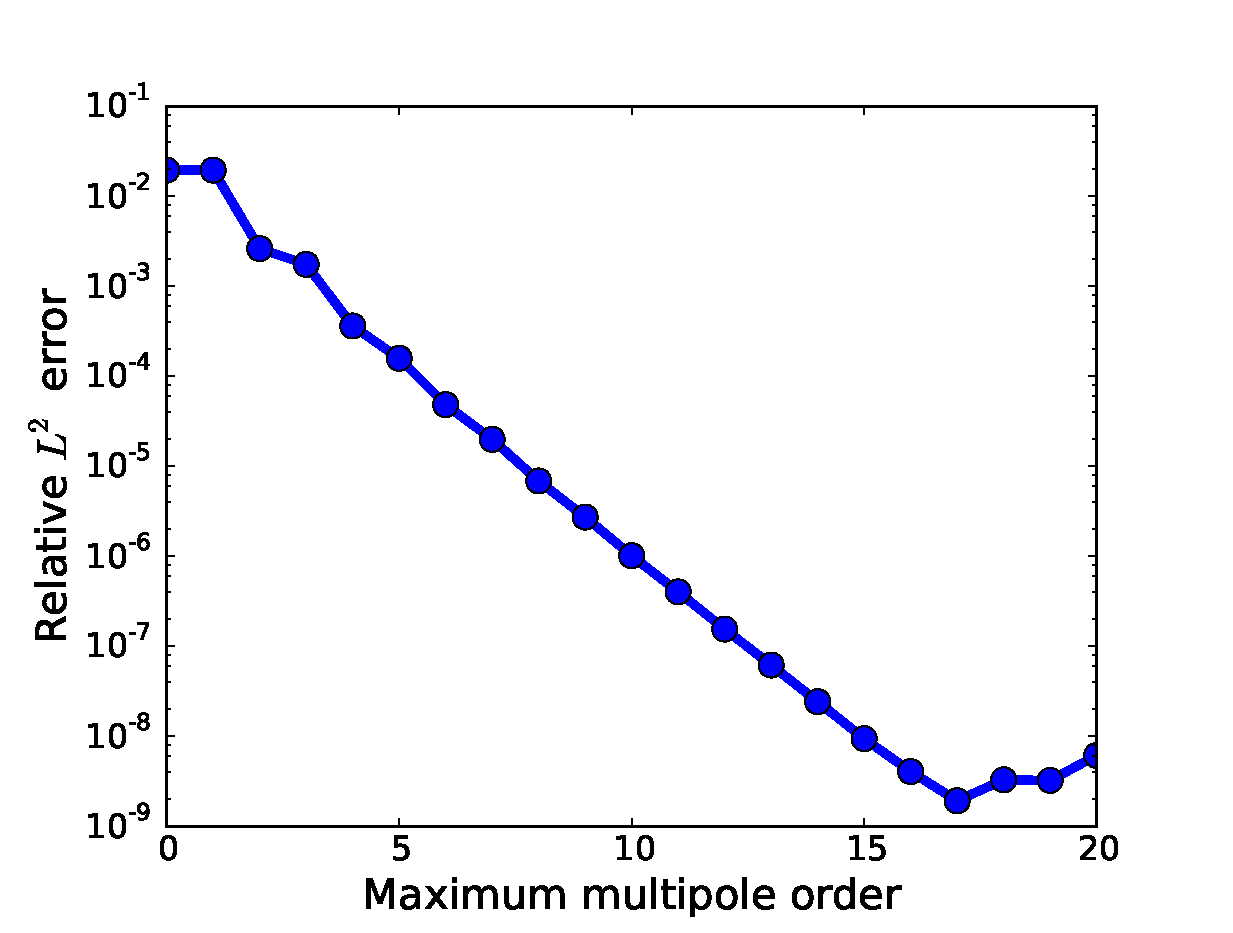
\includegraphics[scale=0.875]{plots/bc_comparison}
  \caption[Error in potential from multipole boundary conditions]
          {Error of $\Phi$ on the computational domain for a binary white dwarf simulation 
           whose boundary conditions were computed using various values of the maximum multipole order,
           relative to the exact solution determined by a brute force sum on the boundaries.
           Circles represent the error at integer values, and they have been connected by a smooth 
           line to guide the eye.\label{fig:bc_comparison}}
\end{figure}

\clearpage
\subsubsection{Convergence Testing}\label{sec:gravity_convergence_testing}

Since the results of a merger simulation depend strongly on gravity,
it is important to check whether proper numerical convergence is
achieved for the Poisson solver. To do so, we created a simple test
that initializes a sphere of radius $R$ and uniform mass density $\rho$
onto our grid, and used \castro\ to calculate the gravitational
potential $\Phi$ of this setup. We ensure that $R$ is an integer
multiple of the grid spacing, and the center of the sphere is at the
origin. The problem domain for our simulations is $[-1.6\ \text{cm}, 1.6\ \text{cm}]^3$, and
we take $R = 1.0\ \text{cm}$ and $\rho = 10^3\ \text{g cm}^{-3}$. 
The zones with $r > R$ are filled with an ambient material of very low density 
($10^{-8}\ \text{g cm}^{-3}$). We run this problem at multiple 
resolutions corresponding to jumps by a factor of two. For
comparison, at each grid point we evaluate the analytical potential of
a uniform sphere, which can be easily determined using Gauss' law:
\begin{equation}
  \Phi_{\text{sphere}}(r) = -\frac{GM}{r} \times \begin{cases} (3R^2 - r^2)/(2 r^2) & r \leq R \\ 1 & r > R \end{cases},\label{eq:sphere-analytical}
\end{equation}
where $M = 4\pi R^3 / 3$ is the mass of the sphere. We measure the 
numerical error by calculating the $L^2$ norm of the error and 
normalizing it by the $L^2$ norm of the analytical solution:
\begin{equation}
  \text{Error} = \frac{\|\Phi - \Phi_{\text{sphere}}\|_2}{\|\Phi_{\text{sphere}}\|_2}.
\end{equation}
We define the order of convergence $p$ between two simulations with a jump 
in resolution of integer factor $m > 1$ as
\begin{equation}
  p = \text{log}_{m}\left(\frac{\text{Error}_{\text{low}}}{\text{Error}_{\text{high}}}\right).
\end{equation}
Here $\text{Error}_{\text{low}}$ is the $L^2$ error at the lower resolution 
and $\text{Error}_{\text{high}}$ is the $L^2$ error at the higher resolution.
We expect the error to converge at $p = 2$ given the discretization we choose. 
For all simulations in this section and for all our main science simulations,
we choose a relative error tolerance of $10^{-10}$ to be satisfied in the multigrid solve.
The results of this test are plotted in \autoref{fig:gravity_convergence}. 

We find that at low resolution convergence is actually substantially better 
than second-order. The explanation for this is that we are attempting to 
model a spherical object on a rectangular grid. This results in two sources of error.
First, at very low resolution, the object does not look very spherical due to the rectangular 
grid representation, so the potential it produces is not quite that of a sphere. 
As the resolution is increased, the distribution of the mass on the grid will change.
\begin{figure}[h!]
  \centering
  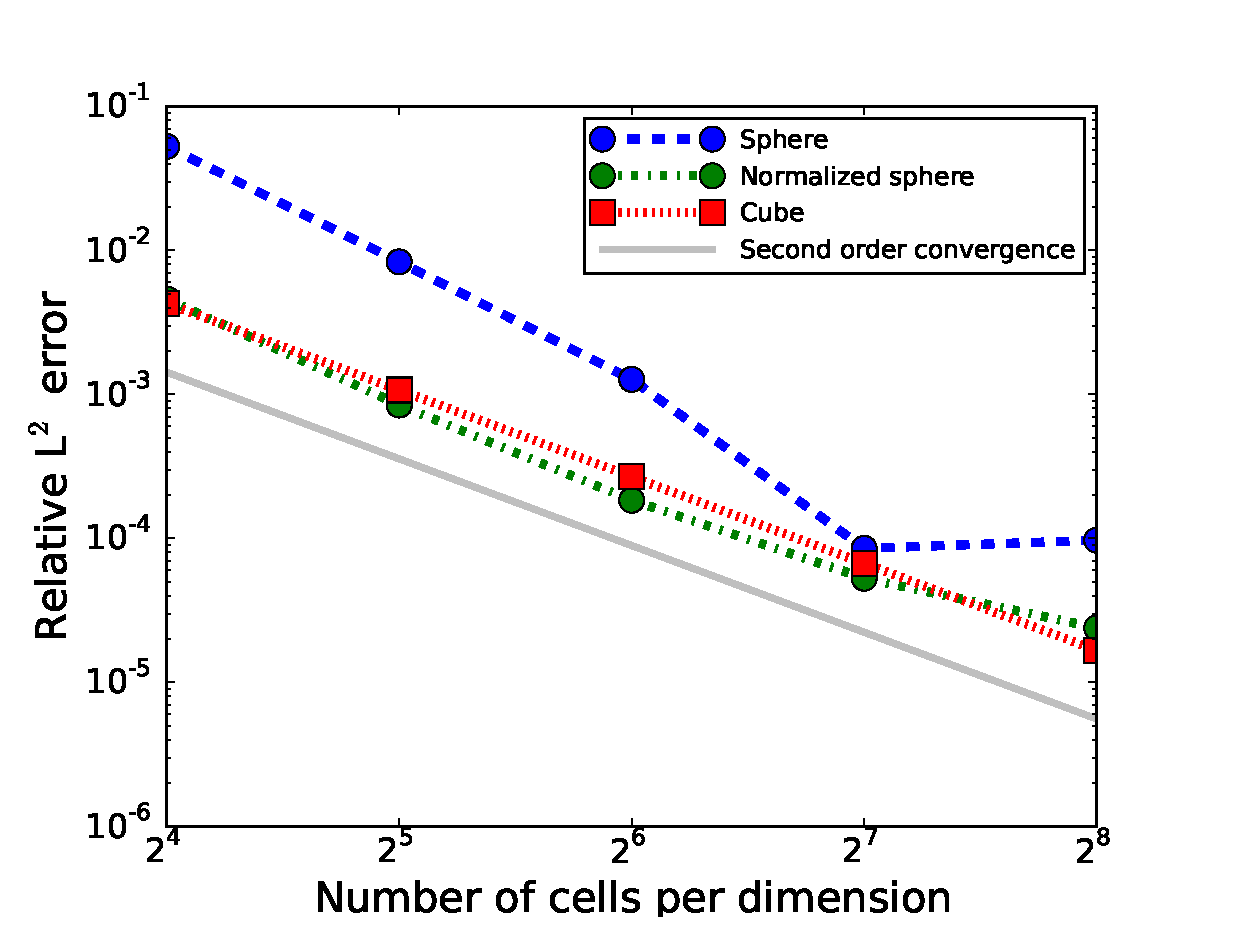
\includegraphics[scale=0.85,trim=0.075in 0.0in 0.7in 0.0in,clip]{plots/phi_comparison}
  \caption[Analytical versus numerical solution of the potential]
          {Comparison of the \castro\ gravitational potential to the analytical solution for: 
           a sphere of uniform density; the same sphere, but with the potential normalized using the 
           actual amount of mass on the grid instead of the mass of a perfect sphere; and, a 
           cube of uniform density. Plotted also is a notional curve whose slope represents
           perfect second order convergence.\label{fig:gravity_convergence}}
\end{figure}
Second, the total amount of mass on the grid will change as the sphere fills out. 
So we are combining the true accuracy bonus from increased resolution 
with the artificial accuracy bonus from getting closer to solving the problem 
we are supposed to be solving. At high resolution this effect levels off, though, 
as the representation of the sphere is not significantly different in 
our two highest resolutions shown. For example, at $128$ zones per dimension 
the amount of mass on the grid happens to be slightly closer to the true spherical 
mass than at $256$ zones per dimension.
We can eliminate the second source of error by changing the density on  
the grid so that the total mass $M$ is actually what we intend it to be.
The resolution study for this case (the ``normalized sphere'') is also
plotted in \autoref{fig:gravity_convergence}. At low resolution we still obtain
convergence slightly better than second-order, indicating that we 
have not eliminated the geometrical problem of the mass distribution changing.

The only way to fully eliminate this effect is to use a test problem that
does not change with resolution. The obvious companion problem is a cube of
uniform density $\rho$, where now $R$ is half of the side length of
the cube. At each resolution we use the same $R$ as for the sphere,
which ensures that the cube always fills exactly the same fraction of
the domain and thus has the same mass, so the only improvement comes
from better sampling at higher resolution. The gravitational potential for this
object has been worked out analytically by \citet{waldvogel:1976} (see
also a similar result by \citet{hummer:1996}, and an earlier calculation 
by \citet{macmillan:1958}). The potential is given in
Equation 15 of that paper\footnote{The last term in that equation is missing a factor of
$1/2$, which destroys the symmetry. We have inserted this missing factor and
performed a simple coordinate transformation so that the center of
the cube is at the origin.}:
\begin{align}
  \Phi_{\text{cube}}(x,y,z) &= -G\rho\sum_{i,j,k=0}^1\left[x_i y_j\, \text{tanh}^{-1}\left(\frac{z_k}{r_{ijk}}\right)\right. \notag \\
  &+ \left. y_j z_k\, \text{tanh}^{-1}\left(\frac{x_i}{r_{ijk}}\right) + z_k x_i\, \text{tanh}^{-1}\left(\frac{y_j}{r_{ijk}}\right) \right.\notag \\
  &\left. - \frac{x_i^2}{2}\,\text{tan}^{-1}\left(\frac{y_j z_k}{x_i r_{ijk}}\right) - \frac{y_j^2}{2}\,\text{tan}^{-1}\left(\frac{z_k x_i}{y_j r_{ijk}}\right) \right. \notag \\
  &- \left. \frac{z_k^2}{2}\,\text{tan}^{-1}\left(\frac{x_i y_j}{z_k r_{ijk}}\right)\right]
\end{align}
where $x_0 = R + x$, $x_1 = R - x$, $y_0 = R + y$, 
$y_1 = R - y$, $z_0 = R + z$, $z_1 = R - z$, 
and $r_{ijk} = \sqrt{x_i^2 + y_j^2 + z_k^2}$. We note that if implemented in 
\texttt{Fortran} or \texttt{C}/\texttt{C++}, the inverse hyperbolic tangent used here is
\texttt{atanh} and the inverse tangent is \texttt{atan} (\textit{not} the more common
\texttt{atan2}). This formula is valid both inside and outside the
cube. The normalized $L^2$ error for this problem is also shown
in \autoref{fig:gravity_convergence}, and only for this problem 
do we obtain perfect second-order scaling at all resolutions.

The main lesson here is that in a convergence study, it is important
to ensure that the physical problem does not change with
resolution. Since in the case of spherical objects on rectangular
grids the effect may be to artificially boost convergence with resolution,
in a simulation with spherical objects like stars one can envision a
scenario of being fooled into believing apparently good convergence
results that are simply a convolution of artificially high
gravitational convergence and poor convergence in the hydrodynamics. A
convergence study in this case is only fully valid if there is reason
to be confident that this effect is negligible compared to other
factors.

\subsection{Rotation}
\label{sec:rotation}

For the evolution of binary systems, it is most natural to evolve the
two stars in a frame that is co-rotating at the same period as the
orbital period. Since the publication of the original code paper, \castro\ 
now has the ability to evolve systems in a rotating reference frame. 
Source terms corresponding to the Coriolis and centrifugal force terms
are added to the momentum and energy equations. In this frame, the stars
essentially remain stationary in their original positions due to the
centrifugal force supporting against the gravitational attraction, and
will remain this way until significant mass transfer occurs. \cite{swc:2000}
demonstrated (in the context of neutron star mergers) that conservation of
angular momentum is much easier to obtain in the rotating reference frame
than in an inertial frame in which stars advect large amounts of material
around the domain. So the use of a rotating reference frame is similar in
motivation to the use of the hybrid advection equations of \autoref{sec:hybrid_advection}.
As the extent to which angular momentum conservation is violated in our code
is a function of the resolution, when the resolution is sufficiently high, 
excellent conservation properties can result, lessening the need for
approaches such as the rotating frame or the hybrid equations. Nevertheless,
at moderate resolution in an inertial frame, there is a secular loss of angular 
momentum that eventually will result in a spurious merger.
We note that as the stars begin to coalesce, the rotating reference frame
will no longer provide a good approximation to the spatial motion of
the stars and then they will begin to significantly move around the
domain. This is not necessarily problematic because the most important
feature of the rotating frame is that it helps ensure that the initial
coalescence is not the result of spurious numerical loss of angular
momentum. When significant mass transfer sets in and evolution
proceeds on a dynamical timescale, the rotating frame may no longer be the
best choice, but should still yield quite reasonable results. In passing,
we note that for this reason, some groups (e.g. \citet{pakmor:2012:gadget})
have opted to perform the early evolution in the rotating frame and then
transform to the inertial frame once mass transfer sets in; we do not
adopt this approach in the current work, but may experiment with it in
the future.

In a rotating reference frame with angular frequency vector $\bm{\omega}$,
the non-inertial contribution to the momentum equation is\footnote{In general there
also a term corresponding to the time rate of change of the rotational frequency,
$\dot{\bm{\omega}}$; we have implemented the ability to use a time-changing
rotational frequency in \castro\ but do not discuss it in this dissertation.}:
\begin{equation}
  \left.\frac{\partial(\rho \mathbf{u})}{\partial t}\right|_{\text{rot}} = -2\, {\bm\omega} \times (\rho\mathbf{u}) - \rho {\bm\omega} \times \left({\bm\omega} \times \mathbf{r}\right).
\end{equation}
Here $\mathbf{r}$ is the position vector with respect to the origin. Typically we choose $\bm{\omega} = (0, 0, 2\pi / T)^T$,
with the rotation axis coincident with the $z$ axis at $x = y = 0$.
$T$ is the rotation period, which is the most natural quantity to specify
for a rotating stellar system. As described in Appendix A of \cite{wdmergerI}, we include this source term
in the edge state prediction in a way that is analogous to the gravity source.
We evaluate all quantities at cell centers. We use the same predictor-corrector 
approach that we use for the gravity source terms to the momentum equations. A slight 
difference is that the Coriolis force for each velocity component is coupled to other velocity 
components. If the rotation is about the $z$-axis, then the discrete update to 
$u^{n+1}$ depends on the value of $v^{n+1}$, and vice versa. If we fix the value of 
the time-level $n+1$ quantities after coming out of the hydrodynamics update, there 
would be a slight inconsistency between the $x$ and $y$ components of the velocity. 

We propose a more accurate coupling that directly solves this implicit system of coupled 
equations. We denote by $(\widetilde{\rho \mathbf{u}})$ the value of the momentum after 
updating it with the centrifugal force, and the time-level $n$ Coriolis force. The remaining 
update for the time-level $n+1$ Coriolis force then appears as:
\begin{equation}
  (\rho \mathbf{u})^{n+1} = (\widetilde{\rho\mathbf{u}}) + \frac{\Delta t}{2} \left(-2\, {\bm\omega} \times (\rho\mathbf{u})^{n+1}\right)
\end{equation}
To proceed further, we assume that the rotation is about the $z$ axis with frequency $\omega$. 
Then there is no update to the $z$-momentum, and the other equations are:
\begin{align}
  (\rho u)^{n+1} &= (\widetilde{\rho u}) + \omega \Delta t (\rho v)^{n+1} \\
  (\rho v)^{n+1} &= (\widetilde{\rho v}) - \omega \Delta t (\rho u)^{n+1}
\end{align} 
We can directly solve this coupled system:
\begin{align}
  (\rho u)^{n+1} &= \frac{ (\widetilde{\rho u}) + \omega \Delta t (\widetilde{\rho v})}{1 + \omega^2 \Delta t^2} \\
  (\rho v)^{n+1} &= \frac{ (\widetilde{\rho v}) - \omega \Delta t (\widetilde{\rho u})}{1 + \omega^2 \Delta t^2}
\end{align}
We use this form of the momentum update in \castro. This improvement is small
but increases the accuracy of our rotating white dwarf systems over long time-scales.

The update to the energy equation can be determined by taking the dot product of the velocity
with the momentum source terms. The Coriolis term vanishes identically, and so
the Coriolis term does no work on the fluid. The update from the centrifugal force becomes
\begin{equation}
  \left.\frac{\partial(\rho E)}{\partial t}\right|_{\text{rot}} = \frac{1}{\Delta V}\int \rho \mathbf{u} \cdot \mathbf{f}^R\, dV,
\end{equation}
with $\mathbf{f}^R \equiv  -{\bm\omega} \times \left({\bm\omega} \times \mathbf{r}\right)$. 
This expression is identical in form to the gravity source under the interchange of $\mathbf{g}$ with $\mathbf{f}^R$.
As observed by \cite{marcello:2012}, we can similarly write down a rotational potential,
\begin{equation}
  \Phi^R = \frac{1}{2} \left| {\bm\omega} \times \mathbf{r} \right|^2.
\end{equation}
In the presence of rotation the conserved total energy becomes:
\begin{equation}
  \int dV (\rho E_{\text{tot}}) = \int dV \left( \rho E + \frac{1}{2} \rho \Phi + \rho \Phi^R \right).
\end{equation}
Given that we can write down a potential energy for the rotation field, then we can use the machinery of 
\autoref{sec:gravity_hydro_coupling}. We again continue to evolve explicitly an equation for 
the gas energy, and allow it to change in response to work done by or on the rotational potential.
\begin{align}
  \left.\Delta(\rho E)\right|_{\text{rot}} &= -\frac{1}{2}\sum_{f} \Delta \rho_{f} (\Phi^R_{f+1/2} - \Phi^R_{f-1/2})
\end{align}

We apply the rotational forces after the gravitational forces, but 
there is some freedom in the order in which to apply the gravitational and rotational terms.
This order may matter because the Coriolis force depends on the fluid velocity, and 
in the predictor-corrector approach, we use the velocities both at 
time-level $n$ and time-level $n+1$. If we update the latter with the gravitational force, 
then the Coriolis force sees a different velocity than the one obtained through the 
pure hydrodynamics step. (The energy equation does not face the same issue in our new formulation,
because the velocities used are always the time-level $n+1/2$ values coming from the Riemann solver.)
This likely does not matter significantly for our simulations in this work because it is
a high order effect, but this issue may be worth exploring in future work.

In simulations performed in a rotating reference frame, we transform all relevant
quantities back to the inertial reference frame when reporting them in analysis routines 
and visualization (except for \autoref{sec:mergers}), though the data is saved to plotfiles
while still in the rotating frame. In particular, for every zone we adjust the position,
momentum, and energy to account for rotation. If the position is $\mathbf{x}$ in the inertial
frame and $\mathbf{x}^\prime$ in the rotating frame, and the rotation vector is $\bm{\omega}$,
the transformation rules are:
\begin{align}  
  \mathbf{x}(t) &= \mathbf{R}\mathbf{x}^\prime(t) \\
  \mathbf{v}(t) &= \mathbf{v}^\prime(t) + \bm{\omega} \times \left(\mathbf{R} \mathbf{x}^\prime(t)\right)
\end{align}
The rotation matrix $\mathbf{R}$ is:
\begin{align}
  \mathbf{R} &= \mathbf{R}_z({\bm{\theta}}_3) \mathbf{R}_y({\bm{\theta}}_2) \mathbf{R}_x({\bm{\theta}}_1)
\end{align}
where $\mathbf{R}_x$, $\mathbf{R}_y$, and $\mathbf{R}_z$ are the standard rotation matrices about 
the $x$, $y$, and $z$ axes, and $\bm{\theta} = \bm{\omega} t$.



\subsection{Nuclear Network}
\label{sec:network}

\subsubsection{Nuclear Isotopes}
\label{sec:isotopes}

White dwarfs are mainly composed of $\alpha$-chain particles, primarily ${}^4$He,
${}^{12}$C, ${}^{16}$O, ${}^{20}$Ne, and ${}^{24}$ Mg, where the $\alpha$ particle
is a ${}^4$He nucleus and the $\alpha$ chain is the series of isotopes obtained by
successive captures of an $\alpha$ particle. Therefore the core of
any network appropriate for modeling nuclear burning in white dwarfs will be
these alpha chain nuclides, with the idea being that links up the $\alpha$-chain
will eventually get us to ${}^{56}$Ni, the nuclide responsible for the
energy output of Type Ia supernovae. In this dissertation we consider four networks
to do this, presented in order of increasing complexity. The most simple is
\isoseven\ \citep{timmes:2000}, which includes all of the aforementioned isotopes and
${}^{28}$Si (see also \citet{hix:1998}). ${}^{28}$Si effectively measures the
equilibrium state of silicon-group elements, and ${}^{56}$Ni effectively measures
the equilibrium state of iron-group elements, with the link between them governed
by the effective loss or gain of seven $\alpha$-particles. This type of network
was used by \citet{rosswog:2009} for their collision calculations in SPH.

Next is \aproxthirteen\ \citep{timmes:1999,timmes:2000}. This includes
all of the isotopes of \isoseven, and all of the $\alpha$-chain particles between
silicon and nickel (${}^{32}$S, ${}^{36}$Ar, ${}^{40}$Ca, ${}^{44}$Ti, ${}^{48}$Cr,
and ${}^{52}$Fe). This network was used in collisions by \citet{hawley:2012} and
\citet{raskin:2010}; \citet{loren-aguilar:2010} and \citet{garcia-senz:2013} used a
very similar network that included additionally ${}^{60}$Zn. It has also been used in mergers
by \citet{raskin:2012,raskin:2014}. \aproxthirteen is the default network used by our
software and is used in the simulations below unless otherwise stated. The \aproxnineteen\
network \citep{timmes:1999} builds on \aproxthirteen\ by including isotopes for
hydrogen burning and explicit tracking of photodisintegration into ${}^{54}$Fe.
This network was used by \citet{kushnir:2013}, \citet{kushnir:2014}, and \citet{rosswog:2009}
for their collision calculations with \flash\ (a commonly used compressible hydrodynamics code
in the astrophysics literature), and \citet{papish:2015}. Finally we will also
consider \aproxtwentyone, which includes all of the above plus ${}^{56}$Cr
and ${}^{56}$Fe and related reaction links. The primary virtue of using
the latter two networks is that they allow us to track changes away from
$Y_e = 0.5$.

All four of these networks have been ported into a form that is consistent
with the \boxlib\ codes, in the freely available \microphysics\ code
repository\footnote{\microphysics\ can be obtained at \url{https://github.com/BoxLib-Codes/Microphysics},
and is also where we store our version of the Helmholtz equation of state.},
a collection of microphysical routines that are designed to be used in our
hydrodynamics codes. These can be easily swapped at compile time by using the 
appropriate makefile variable.



\subsubsection{Nuclear Burning}
\label{sec:burning}

Given a set of nuclides and the reaction links between them, we now consider
how a burning step is performed in our software. The goal is to integrate the
vector ${\bm{Y}} = (Y_1, Y_2, \ldots, Y_n, e, T)$, where $Y_{n} = X_{n} / A_{n}$
is the molar fraction of species $n$, with $X_n$ the mass fraction and $A_n$ the
mass number of that species, $e$ is the energy released during the burn, and
$T$ is the temperature. The equation describing its evolution is given by
\begin{equation}
  \frac{d\bm{Y}}{dt} = f(\mathbf{Y}),
\end{equation}
where the components of the right-hand-side for the species come from the particular
nuclear burning network we are using. The energy $e$ of the zone
will change when the nuclear abundances evolve, according to
\begin{equation}
  \frac{\partial e}{\partial t} = N_A \sum_{n} \frac{\partial Y_{n}}{\partial t} m_{n} c^2,
\end{equation}
where $c$ is the speed of light and $m_n$ is the mass of each nuclide.

We define several burning modes that determine how $T$ and $e$ are evolved
during a nuclear burn. In a hydrostatic burn, which we call burning mode 0,
we keep $\rho$ and $T$ fixed throughout, and use
the energy released at the end to compute a final temperature that is
thermodynamically consistent with the new internal energy. By contrast,
in a self-heating burn (mode 1), we allow the temperature to evolve in response
to the burning (see\footnote{In the cited paper, a term based on the
thermodynamic chemical potential was included; we now believe
that it is incorrect to include such a term in the burn, since it
automatically sums to zero analytically.} \citet{maestro3}):
\begin{equation}
  \frac{dT}{dt} = \frac{1}{c_V}\frac{\partial e}{\partial t}
\end{equation}
(Although $T$ evolves during the burn so that the integration is physically
accurate, as in the hydrostatic method we discard the final value
for $T$ at the end of the burn and recompute a temperature for the zone that is
consistent with its new internal energy.) Here $c_V$ is the specific heat at
constant volume, which is provided by the equation of state.  During this burn,
we can keep $c_V$ constant using its initial value, or at each step we
can choose to re-evaluate the equation of state using the latest value of $(\rho, T)$.
The latter is more expensive but also more accurate, and we use it in this dissertation.
In practice we find that the cost is small in comparison to the more expensive
parts of the calculation, and it can significantly speed up convergence near NSE.
A third option (mode 2) presented by \citet{raskin:2010} is a so-called ``hybrid'' mode.
In this mode, by default we do a hydrostatic burn. If that burn fails, or if the net
energy change is negative, we do the burn again in self-heating mode. A final option
is a burn that limits the changes due to a burn to avoid numerically unstable burning.
This mode is discussed in \autoref{sec:unstable_burning} and we will call it a
``suppressed'' burn (mode 3) for the remainder of this work. All four options
are implemented in our burner software. The simulations shown in this work all
use the self-heating mode unless otherwise specified.

In our \microphysics\ repository we provide several software options for solving a set
of coupled stiff ODEs. For this work we use an implementation of the well known variable-order
Richardson extrapolation method presented by \citet{stoer:1980}, that is similar to the
integrator which ships with the original versions of the networks mentioned above.
Previous work using the \boxlib\ codes typically used the \vode\ integrator \citep{vode}.
We do maintain a version of the software that is compatible with our software interfaces
in the \microphysics\ repository, but we have largely shifted to integrators which are
written in modern Fortran as a consequence of our efforts to run our codes on GPUs.
The Stoer and Bulirsch integrator we provide satisfies this criterion; we also provide
a rewrite of the VODE BDF algorithm that uses modern Fortran features. The Stoer and
Bulirsch algorithm relies on a uniform relative error tolerance for all of the ODEs
in the system, which we set at $10^{-6}$ for all simulations described here.



\subsubsection{Coupling Burning to Hydrodynamics}
\label{sec:burnerhydrocoupling}

In \castro, the reactions are coupled to the hydrodynamics using Strang splitting.
In a given timestep advance $\Delta t$, we first evolve the reactions alone through
a time interval $\Delta t / 2$. Then, we evolve the hydrodynamics for $\Delta t$,
and we evolve the reactions again for a further $\Delta t / 2$. The principal
drawback of this approach is that the reactions and the hydrodynamics can become
decoupled from each other. A common solution to this problem presented in
the literature has been to limit the size of the timestep and thereby limit the
extent of this decoupling \citep{raskin:2010,hawley:2012}, which we adopt here 
and have implemented in \castro. Defining the nuclear energy injection timescale 
$\tau_e$, and the species evolution timescale $\tau_{X_k}$,
\begin{align}
  \tau_e &\equiv \frac{e}{|\dot{e}|} \\
  \tau_{X_k} &\equiv \frac{X_k}{|\dot{X_k}|},
\end{align}
where $\dot{e}$ is an estimate of the time rate of change of the internal energy
from nuclear burning, and $\dot{X_k}$ is an estimate of the time rate of change 
of the mass fraction of the species with index $k$, we define burning-limited 
timesteps $\Delta t_{be}$ and $\Delta t_{bX_k}$:
\begin{align}
  \Delta t_{be} &= f_{e}\, \tau_e \label{eq:timestep_e}\\
  \Delta t_{bX_k} &= f_{X}\, \tau_{X_k}. \label{eq:timestep_X}
\end{align}
Given an estimate for $\dot{e}$, the factor $f_{e}$ determines by what 
fraction we would like to allow the internal energy to change
in the current timestep, under the assumption that $\dot{e}$ does not change from
timestep to timestep. Similarly, given an estimate for $\dot{X_k}$, the factor $f_{X}$ 
determines the maximum change in the mass fraction of any species. By making 
$f_{e}$ and $f_{X}$ smaller, we can control the magnitude of the decoupling 
between the reactions and the hydro. A typical choice for $f_e$ parameter in the
literature is in the range of 0.2 or 0.3, while to our knowledge a limiter based on
$f_X$ has not been used by others performing these types of calculations. The sensitivity
of results to the value of these timestep limiters will be discussed in
\autoref{sec:collision_parameters:timestepping}. The factors $f_{e}$ and $f_{X}$ can be set at runtime in \castro.

At the start of each advance, we limit the size of the timestep to be the smaller
of the minimum hydro timestep (limited by the CFL condition), and the minimum of all the
burning timesteps across all zones. To do this, we need a method for determining 
$\dot{e}$ and $\dot{X_k}$. A typical choice in the literature has been to set, for example,
\begin{equation}
  \dot{e} = \frac{e^{n} - e^{n-1}}{\Delta t^{n-1}}, \label{eq:burning_limiter_mode_4}
\end{equation}
where is $e^n$ is the internal energy at the start of the current timestep and
$e^{n-1}$ is the internal energy at the start of the previous timestep. 
The obvious analogue is used for constructing the species rate of change.
However, there are alternative methods of constructing this derivative estimate, 
and we have found that these different methods have measurable consequences.
We define four separate methods for calculating the time derivative, with 
the above being mode 4. Mode 3 is similar to mode 4 but replaces the
denominator in \autoref{eq:burning_limiter_mode_4} with the change in 
internal energy over the last timestep only from the nuclear reactions.
Mode 2 is the same as mode 3 but we only use the change in internal 
energy from the most recent nuclear burning step, that is, the second-half
of the Strang-split burning from the last timestep (the denominator 
then becomes $\Delta t / 2$). In mode 1, the most accurate option and 
the current default in \castro, we evaluate the right-hand-side of the 
burning network given the current state to explicitly obtain the 
instantaneous value of $\dot{e}$ and $\dot{X_k}$. 

To understand the consequences of this choice, and more broadly to 
understand the limitations of Strang splitting, we consider the 
basic outline of a single-level advance in an advection-reaction system:
\begin{enumerate}
  \item Evaluate timestep $\Delta t$ for the current advance
  \item Advance the nuclear burning network by $\Delta t / 2$
  \item Advance the hydrodynamics by $\Delta t$
  \item Advance the nuclear burning network by $\Delta t / 2$
  \item Return to Step 1
\end{enumerate}
Now, consider that during a head-on collision, initial nuclear burning 
will occur at the contact point between the two stars. Because of 
the staggered updates from splitting, the evolution effectively progresses 
as a cycle between burning for $\Delta t$ and getting fresh material 
advected into the contact point by the hydro update for $\Delta t$. 
When the collision begins, $\Delta t$ is controlled by the hydrodynamic 
stability criterion, and may be large enough that it is possible for 
the burning advance in Step 4 to completely burn the freshly advected 
material all the way to NSE. Consequently the evolution is no longer 
a good approximation to smooth burning of the in-falling material but
rather separate discrete burning and hydro steps, and the nature of 
the burning evolution will be quite different. Furthermore, by the 
time we return to Step 1 and estimate the next timestep size, all 
of the burning rates will be small again, and the instantaneous 
timestep limiter of mode 1 may actually substantially overestimate 
the needed timestep. The other modes will see that the energy/species  
substantially changed over the last timestep, but will still 
overestimate the needed timestep because the burning was quiescent
for at least some portion of the last advance. Our experience has
shown that none of these methods is flawless, and that limiting
based on only changes in internal energy is particularly susceptible
to this staggered burning phenomenon; silicon-group material can
build up without changing the internal energy by a  large fraction,
so the timestep limiter is never triggered, and then in a single step
a substantial amount of iron-group elements can be be generated,
perhaps forming a detonation. This can have non-trivial effects
on the total amount of iron-group elements generated over the course of
the simulation. We have found that the addition of the 
limiter based on changes in species functionally precludes this, and
so the two methods can complement each other.

With the timestep limited the way we advocate in this dissertation, 
the timesteps are generally short enough so that the errors 
due to splitting are small. (Note that the timestep limiting is
most crucial at low resolution; higher resolution automatically demands
shorter timesteps due to the CFL criterion.) Other approaches to the coupling 
between reactions and hydrodynamics have been proposed in the 
broader literature, especially iterative methods such as 
deferred corrections that allow each of these operators to 
feel the lagged effects of the other operators. For example,
in the context of low Mach number flows, \cite{nonaka:2012} have
used the method of spectral deferred corrections \citep{SDC} to
couple their advection-diffusion-reaction equation set. In our
context this would involve treating the full evolution equation
for each of the state variables as an ODE with a directly coupled
burning source term integrated at high order; the advective
flux is evaluated at the standard second order accuracy
and is included as an ODE source term.
We are presently investigating such a method,
and it may form the basis of further work on this subject.

Now we return to a point we hinted at above. The timestep
will only actually satisfy the energy criterion
$\Delta t \leq f_e \tau_e$ and species criterion
$\Delta t \leq f_{X_k} \tau_{X_k}$ when the estimates for
$\dot{e}$ and $\dot{X_k}$ we generate are at least as large
as the actual rate of change of energy and mass fractions
over the timestep. However, this can assumption can fail
during periods of runaway burning when the rate of change
of these quantities is highly nonlinear. We may not want
to neglect the errors caused by this approximation
because they may build up over an extended period of nonlinear
evolution and perhaps substantially change the final results.
To this end, we have implemented a timestep retry option in
\castro, which re-computes an advance if it violated the
stability criteria as judged from the end of the timestep.
However we have found that the benefits for this problem are
small and thus we do not use it for the simulations here.

One other point worth noting for the coupling of the reactions
and the hydrodynamics relates to the dual-energy formalism used
by \castro\ and many other hydrodynamics codes \cite{bryan:1995}.
\castro\ evolves separately equations for the total energy $(\rho E)$ and
for the internal energy $(\rho e)$. The former is conservative while the latter
is not, so for accurate hydrodynamics we prefer to use the total
energy when possible and to use the evolved internal energy variable
only in situations where the kinetic energy dominates the contribution
to the total energy. Indeed, for the cosmological purpose for which
this was originally developed, \cite{ENZO} choose a value $\eta_2 = 0.1$
so that $e$ is only updated to be equal to $E - \mathbf{v}^2/2$ if
$e > \eta_2\, E$. In other cases the evolved value of the internal
energy variable is preserved. However, this choice is somewhat unsafe
for our application, because the ultimate cause of the nuclear
burning in a white dwarf merger or collision is the rapid conversion of
kinetic energy from the white dwarf bulk motion to thermal energy
as the white dwarfs slam into each other. Keeping $\eta_2$ large
prevents this from happening, and consequently the temperature
will never reach values high enough to generate significant
amounts of nickel. For this dissertation we choose $\eta_2 = 10^{-4}$,
which is low enough for the correct conversion of kinetic energy
but not so low that we need to be concerned about roundoff issues
caused by subtracting kinetic from total energy. This is also
the value that was used by \cite{hawley:2012}.

\subsubsection{Numerically Unstable Burning}
\label{sec:unstable_burning}

\citet{kushnir:2013} point out that an inappropriate timestep is 
not the only way for the numerical discretization to cause 
severe errors in the burning. Another failure mode is when
the energy injection timescale
$\tau_e$ is shorter than the sound-crossing time $\tau_s$ in a zone.
When the sound-crossing time is too long, energy is built up in
a zone faster than it can be advected away by pressure waves.
This is obviously a problem inherent to numerically discretized
systems as the underlying fluid equations are continuous.
This can lead to a numerically seeded detonation caused by the
temperature building up too quickly in the zone; the detonation
is spurious in this case and should be avoided if possible.
The goal is to ensure that the following condition holds:
\begin{equation}
  \tau_s \leq f_{s}\, \tau_e \label{eq:burning_limiter_2}
\end{equation}
The sound crossing time, $\tau_s$, is given by $\Delta x / c_s$, 
where $c_s$ is the sound speed and $\Delta x$ is the (minimum) 
zone width. The parameter $f_{s}$ then determines the minimum
ratio of the nuclear energy generation timescale to the 
sound-crossing time. \citet{kushnir:2013} choose $f_{s} = 0.1$ 
for their simulations, and we do too (this parameter can be set 
at runtime in \castro).

\citet{kushnir:2013} implemented this criterion by artificially 
limiting the magnitude of the energy release after a burn. We
too have developed an option for our burner to do this,
the ``suppressed'' burning mode. In a suppressed burn, we limit
the changes to the state so that \autoref{eq:burning_limiter_2}
is always satisfied. To achieve this we directly multiply the
right-hand-side vector in the integration by a constant factor $F$
for all variables, where $F$ is the multiplicative factor needed to
be applied to $\dot{e}$ such that the equality in \autoref{eq:burning_limiter_2}
holds. (If the inequality is already satisfied, then the integration
vector is not modified.) We fix $\tau_s$ to be the value of the sound
crossing time at the beginning of the burn (that is, we do not
update it as the sound speed changes) and we fix the energy $e$
that goes into the estimate for $\tau_e$ to be the value of the
internal energy of the zone at the beginning of the burn. If
instead one allowed $c_s$ and $e$ to evolve with the burn, one
would obtain a less conservative limiter in the case of explosive
burning, as $c_s$ and $e$ are both increasing in this case.
As the point of the limiter is to ensure that the changes to the
\textit{original} energy are small enough so that the following
hydrodynamics update can advect away newly generated energy
quickly enough to avoid a numerically seeded detonation,
we desire the most conservative version of the limiter. We discuss
our results with the suppressed burning mode in \autoref{sec:collision_parameters:burningmode}.
Note that we have found that with this option enabled, it typically takes
many more timesteps to complete a burn than in self-heating mode.

Regardless of whether the suppressed burning mode works for this
particular problem, it is not physical, so we include for
consideration a different approach. If we insist that we
cannot directly control the energy injection timescale, we 
must find a way to alter the sound-crossing timescale. 
We can achieve this by adding levels of refinement in 
regions that do not satisfy \autoref{eq:burning_limiter_2},
which effectively lowers $\Delta x$ and thus the
sound-crossing time. We keep tagging zones for refinement
based on this criterion until the criterion is satisfied
on the finest level. Since the concern is regions that 
may detonate, we also tag nearby zones in a buffer region
which do not themselves satisfy the criterion,
so that a detonation in a single timestep cannot 
escape into non-refined regions. The width of the buffer 
region should thus be at least as large as the number of 
timesteps before a regridding procedure is performed.
We choose a value of two for both the number of zones in the 
buffer region and the number of steps in between regrids,
for all simulations in this dissertation.

We agree with \citet{kushnir:2013} that solving this numerical
instability is crucial to avoiding unphysical detonations.
A simulation that does not solve this problem will not obtain
the correct amount and will not converge properly with resolution.
This may justify the addition of many AMR levels to the domain
if a correct evaluation of the burning phase is desired.
Even if one cannot afford the full resolution required by this
AMR criterion, and chooses to limit the number of levels to some
predetermined maximum based on a constraint of computing time,
the added resolution will still go to the most-needed places.
However, a significant drawback to this approach is that it
does not turn on until after an unstable burning region has
been generated, so this AMR criterion cannot help in the case
where a spurious detonation begins in a single timestep on the coarse
grid, though it will kick in immediately after that timestep
to resolve the regions where the detonation has occurred.
A possible remedy to be explored in future work is to add
refinement pre-emptively in regions where the ratio $\tau_s / \tau_e$
approaches $f_{s}$ but does not yet exceed it. Another
possibility for this case would be to track how many levels
would have been needed to prevent the numerical detonation,
based on the stability criterion, and reject the timestep and
retry it from the starting state using that many levels of refinement.
As mentioned in \autoref{sec:burnerhydrocoupling}, the ability to
reject a timestep and retry it is functionality that
we have recently added to \castro, so we may try this in future work.



\newpage
\section{Simulation Software}
\label{sec:software}

In this section we describe the white dwarf merger software, and focus in 
particular on the initial white dwarf models (\autoref{sec:initial_models}), 
the initial problem setup (\autoref{sec:initial_state}), and analysis 
(\autoref{sec:analysis}) components.

The software used to set up the problems in this dissertation
\wdmerger\footnote{\wdmerger\ can be obtained at \url{https://github.com/BoxLib-Codes/wdmerger}.},
is freely available at an online repository hosting service.
\wdmerger\ is effectively a problem setup for \castro\ similar to the types of
problems that come packaged with the software, and also contains tools for setting up
simulations and analyzing the results.
Version control in both the parent software (\boxlib, \castro, \microphysics) and in \wdmerger\
permits us to reference the state of the code at the time a simulation
was performed. In all plot files and diagnostic output generated by \castro, 
and figure files generated by \wdmerger,
we store the active \texttt{git} commit hashes of \boxlib, \castro, \microphysics, and \wdmerger.
Line plots are generated using the \matplotlib\ library for \python\ 
\citep{matplotlib}, while slice plots and other multi-dimensional visualizations are 
generated using the \yt\ code \citep{yt}.



\subsection{White Dwarf Models}
\label{sec:initial_models}

At the start of any full simulation, we generate initial model white
dwarfs by integrating the equation of hydrostatic equilibrium, taking
the temperature to be constant, and using the
stellar equation of state.  This results in a single non-linear
equation to find the density in a zone given the conditions in the
zone beneath it:
\begin{equation}
\frac{p_{i+1} - p_i}{\Delta x} = \frac{1}{2} (\rho_i + \rho_{i+1}) g_{i+1/2}.
\end{equation}
This equation is a function of $\rho_{i+1}$ only since the pressure is
uniquely determined by the density in this case. Here, $\rho_i$ and $p_i$
are known, and $g_{i+1/2}$ is the gravitational acceleration at the
interface between zones $i$ and $i+1$, found by simply adding up all
the mass from zones $1$ to $i$ to get the enclosed mass,
$M_{i+1/2}$, and then setting $g_{i+1/2} =
-GM_{i+1/2}/r_{i+1/2}^2$. We solve this equation for $\rho_{i+1}$
using a Newton-Raphson iteration.

We desire to specify the mass of the white dwarf, as well as its
temperature and composition. To start the integration off, we
therefore need to guess at a central density.  We then do a secant
iteration over the entire integration procedure to find the central
density needed to yield the desired total mass.  The grid spacing is
$\Delta x = 6.25\ \text{km}$. We chose this value because no simulation
we perform is likely to exceed this grid resolution inside the stars 
themselves; for our normal domain size (see below), this corresponds to 
three jumps in refinement by a factor of four. We find that for low 
resolution runs, this is a better choice than selecting the 1D grid 
spacing to be comparable to the 3D grid spacing.

The white dwarf composition is determined by the chosen mass. For 
this dissertation we adopt the scheme of \cite{dan:2012}. Low-mass WDs 
are pure helium; low-to-intermediate-mass WDs are an even carbon-oxygen 
core with a relatively large helium envelope; intermediate-mass 
WDs are a carbon-oxygen core with slightly more oxygen than carbon; 
and, high-mass WDs are composed of oxygen, neon, and magnesium. 
This choice of composition distribution broadly resembles the 
results of stellar evolution calculations in the respective 
mass ranges, though it does not match the calculations in detail.

We map the 1D model onto the 3D Cartesian grid by taking density,
temperature, and composition as the independent variables,
interpolating these to the cell centers, and then calling the equation
of state to initialize the remaining terms. It is possible to interpolate
instead by using pressure instead of temperature, as pressure is more 
closely related to hydrostatic balance, but the EOS we use is so 
insensitive to temperature that this mapping can result in large 
deviations from the isothermal assumption we started with.  The 
interpolation process divides each zone into $n_{\text{sub}}$ 
sub-zones of equal volume for
the purpose of sampling the 1D model, and the sub-zones are added
together to obtain the full zone's state. This
sub-grid-scale interpolation is useful especially near the edge of the star,
where the density falls off rapidly with radius. Typically we take 
$n_{\text{sub}} = 4$.



\subsection{Initial State}
\label{sec:initial_state}

The \wdmerger\ software comes with a robust set of options for setting up
various types of binary white dwarf systems (and it can also do a single
star simulation by placing the star at the center of the computational domain,
which we take to be the origin.) For mergers and other problems that start
the WDs in a circular orbit, the setup is described in \autoref{sec:initial_state:mergers},
while for collisions the setup is described in \autoref{sec:initial_state:collisions}.



\subsubsection{Mergers}
\label{sec:initial_state:mergers}

For a binary star merger simulation that starts in a circular orbit,
we take as parameters the mass of the two white dwarfs and some measure
of the initial distance. The simplest is the initial orbital period $T$.
Using Kepler's third law and assuming a circular orbit, we can then work
out the orbital separation $a$:
\begin{equation}
  a = \left(\frac{GM T^2}{4\pi^2}\right)^{1/3}.
\end{equation}
Here $M = M_P + M_S$ is the total mass of the system, where $M_P$ is
the specified \textit{primary} mass and $M_S$ is the specified
\textit{secondary} mass. The primary WD always starts on the left
side of the computational domain for our simulations, and is more
massive than the secondary. This reflects the usual terminology in the
literature where the primary WD is the accretor and the secondary is
the donor. The center of mass is located at the center of the
computational domain, and by default the stars lie along the $x$ axis, so that
the primary's center of mass is located at $x = -(M_S / M)\, a$ and
the secondary's center of mass is located at $x = (M_P / M)\, a$.
The user may choose to initialize the stars along a different axis,
and can also choose a non-zero orbital phase and/or eccentricity.

For simulations intended to cause a merger, we want a measure that takes
into account the likelihood that mass transfer will begin. The traditional
choice is the Roche radius of the star, which measures the effective gravitational
sphere of influence for each star. The effective Roche radius $r_L$ is defined as
the radius of a sphere that would have the same volume as the Roche lobe, the
region of space in which material principally belongs to one of the stars. (The surface
of the region is the isosurface where the effective potential becomes zero, meaning
that material becomes unbound due to the centrifugal force). It is
an approximation because this region is teardrop-shaped in reality. A common
expression, which we adopt, for $r_L$ is
the formula provided by \citet{eggleton:1983}:
\begin{equation}
  \frac{r_L}{a} = \frac{0.49 q^{2/3}}{0.6^{2/3} + \text{ln}(1 + q^{1/3})}.\label{eq:roche_radius}
\end{equation}
$q \equiv M_S / M_P$ is defined as the mass ratio of the binary system. Since
we specify the mass ratio, we can use this formula to obtain a binary setup where $a$,
the initial separation, is such that the location of the inner edge of the secondary
is coincident with the extent of its Roche radius.
In other words, the secondary is on the brink of mass transfer. We can also multiply this
by a factor $f_R$ to increase or decrease the distance relative to the Roche radius; for
$f_R > 1$ the system gets more stable against mass transfer, and $f_R < 1$ the system becomes
more unstable to mass transfer.

The initial velocity is taken to be zero in if we are in the reference
frame that rotates with the WDs, and if we are in the inertial frame
the velocity in every zone is set equal to the rigid rotation rate 
corresponding to the distance of that zone from the rotation axis, given
the specified period $T$. Thus the inertial frame and rotating frame 
simulations are starting off with the same initial conditions: two white 
dwarfs locked in synchronous rotation. This is the simplest assumption to 
make, but in the future we may explore relaxing this requirement.

In this dissertation we do not attempt to enforce equilibrium with an additional relaxation
step. This will be an important part of future work that follows up on
what we have done here, as numerous groups working on binary evolution
\citep{swc:2000,motl:2002,rosswog:2004,dan:2011,pakmor:2012:gadget}
have commented on the importance of equilibrium initial conditions in
determining the evolution of the system. As a consequence of starting 
in a non-equilibrium setting, there are 
large density and pressure gradients near the white dwarf surfaces
that result in significant amounts of mass flowing out of the white dwarfs.
This can result in spurious non-physical consequences such as 
the total density or energy going negative in a zone. To compensate 
for this, we start the simulation with a timestep that is a few orders 
of magnitude smaller than that required by the CFL criterion, and allow
the timestep to increase by 1\% each timestep so that the timestep reaches 
its maximum allowed by the velocities on the grid over a span of approximately 
1000 timesteps. This allows the gas at the surface of the white dwarf
to come closer to equilibrium without having discontinuous jumps in the
density or energy. For all simulations, the maximum hydrodynamic timestep
is set to be equal to one-half of the CFL limit.

The computational domain has a total size of $1.024 \times
10^{10}\ \text{cm}$ in each spatial dimension, and is centered at the
origin. Our coarse grid has $256^3$ zones, corresponding to a spatial
resolution of 400 km. For all mergers in the present study, we choose a simple
refinement strategy for mergers: on the coarse grid, all zones within
twice the Roche radius of each star are tagged for refinement. The extra
buffer from doubling the Roche radius ensures that the sharp density gradients near
the edge of the star are within the zone of refinement. On higher levels, 
we tag all zones above a given density threshold (taken to be $1\ \text{g cm}^{-3}$ 
in this dissertation) that corresponds to the stars themselves.

Outside of the stars we fill the rest of the domain with a very low density 
ambient gas because our hydrodynamics model requires the density to be 
non-zero everywhere. This ambient material can create difficulties for the simulation.
In addition to negative densities or energies that can be created at the stellar surfaces, 
in the rotating reference frame we observe that standing instabilities can create very 
large velocities in the ambient fluid that drag down the global timestep by 
up to an order of magnitude.  To deal with this we employ a ``sponge'' similar 
to that described by \citet{maestro3} for the outer regions of the computational domain. 
After the hydrodynamics update, we apply a damping force to the momentum
equation as follows:
\begin{equation}
  (\rho \mathbf{u})^{n+1} \to \frac{(\rho \mathbf{u})^{n+1}}{1 + (\Delta t / \Delta t_S) f_S},
\end{equation} 
where $\Delta t_S$ is a timescale for the sponge to operate on, and
$f_S$ is the damping factor.  We choose it so that that the sponge is
non-operational inside a radius $r_S$ from the origin, and fully
applied at a radius $r_S^\prime \equiv r_S + \Delta r_S$. We then
smooth the sponge out between $r_S$ and $r_S^\prime$:
\begin{equation}
  f_{S} = \begin{dcases} 0 & r < r_S \\ \frac{1}{2}\left(1 - \text{cos}\left[\pi\left(\dfrac{r - r_S}{\Delta r_S}\right)\right]\right) & r_S \leq r < r_S^\prime \\ 1 & r \geq r_S^\prime. \end{dcases}\label{eq:sponge_frac}
\end{equation}
For the simulations in this dissertation that use the sponge, we set $r_S$ to be 75\% of the 
distance from the origin to the domain boundaries, and $\Delta r_S$ so
that the sponge smoothing region extends another 10\% of that distance.
The resulting profile is displayed in \autoref{fig:sponge}. We set $\Delta
t_S = 0.01$ s, which is of the same order as the CFL timestep
for typical problem setups. While the sponge is applied we should avoid imputing any physical 
meaning to what is happening in the low-density gas far from the stars. We use the
sponge for the verification tests of \autoref{sec:verification} but do not enable it
for the runs in \autoref{sec:mergers}.
\begin{figure}
  \centering
  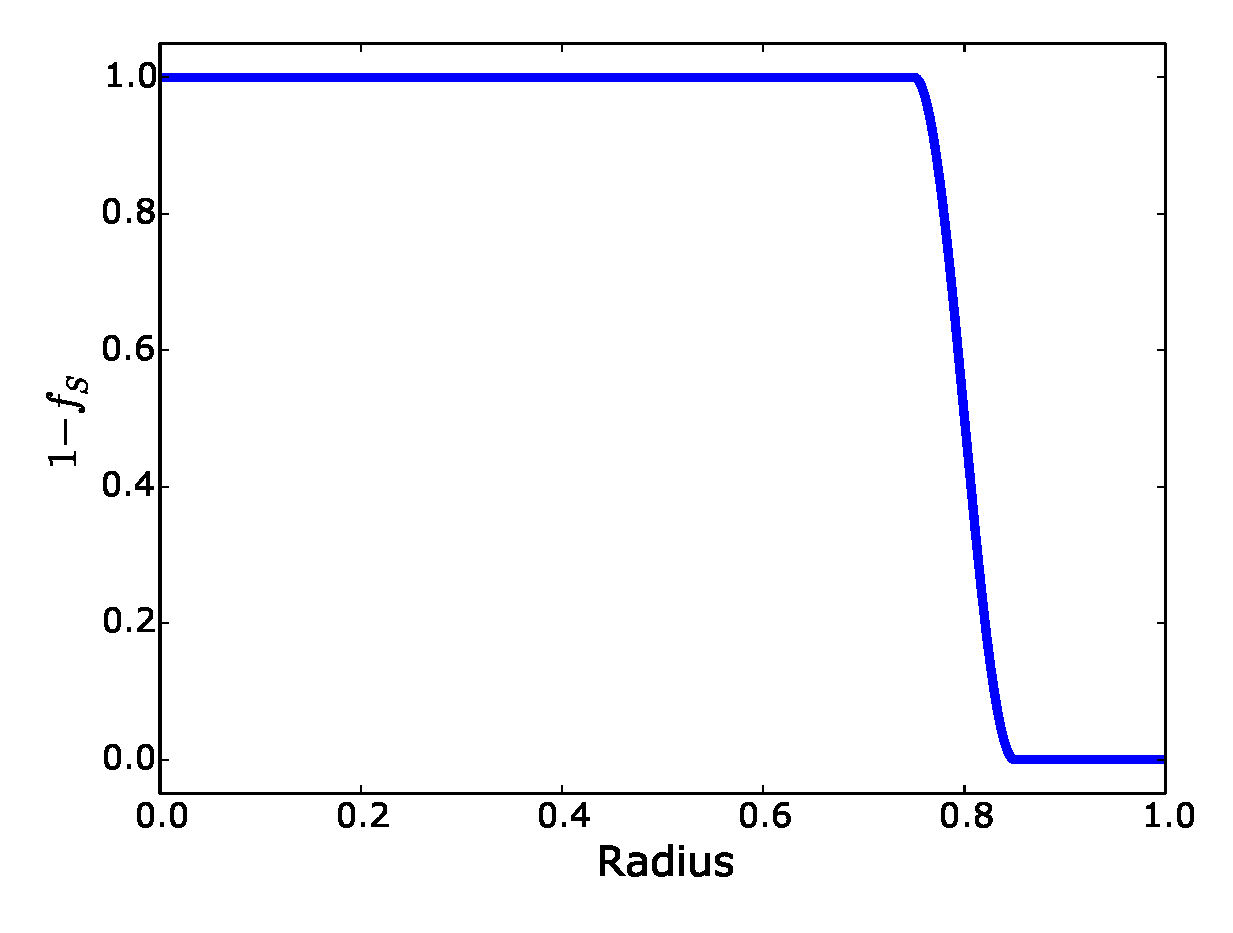
\includegraphics[scale=0.8]{plots/sponge}
  \caption[Radial profile of the hydrodynamical sponge]
          {Radial profile of the hydrodynamical sponge we apply (\autoref{eq:sponge_frac}). 
           We subtract $f_S$ from unity; the value of $1 - f_S$ indicates what happens 
           to the sponged function after the sponge is applied. The sponge has no effect 
           in the inner part of the domain, and is fully applied at the outer edge.
           \label{fig:sponge}
          }
\end{figure}


\clearpage
\subsubsection{Collisions}
\label{sec:initial_state:collisions}

We implement the white dwarf collision problem in \castro\ by setting the white dwarf
centers of mass to be initially separated by a distance of four times
the (secondary) white dwarf radius. (Note that the radius of the white dwarf, and
consequently the initial distance, depends on the equation of state used, and this
can vary somewhat depending on the relevant physics used, such as Coulomb corrections
in the Helmholtz equation of state. However, the results do not really depend on the
exact initial distance as long as there is enough time for the WDs to distort in
response to tidal forces as they approach.) Their initial velocity is that of
two point-masses in free-fall towards each other coming in from infinity, such that
the contact point is at the origin, and they approach each other along the $x$-axis.
By default the WDs approach each other head-on, with their respective centers
lying on the $x$-axis, but we have also added an option
to have the WDs approach each other at a non-zero impact parameter $b$, where the
offset is perpendicular to the $x$-axis in the $y$ direction. We measure
$b$ in units of the secondary WD's radius, so that the default head-on case
corresponds to $b = 0$ and the case where the two WDs just graze past each other
corresponds to $b = 1$ (in practice it happens slightly differently because
of the WDs responding to each other's gravitational fields).

For all the 3D simulations to follow, we use the same coarse grid as in \autoref{sec:initial_state:mergers}.
When we use adaptive-mesh refinement, we will usually
use the refinement scheme described in \autoref{sec:unstable_burning}. This is
acceptable because the outcome of the collision problem is chiefly a function
of the propagation of burning front through the WDs, so for this problem one
can take some liberties in other parts of the algorithm for the purpose of
computational efficiency, which can always be turned back on later if a more
accurate answer is desired. So, for example, we do not need to add refinement
everywhere in the WDs in the interest of getting the collision dynamics to be
slightly more accurate. Additionally, we choose to solve the Poisson equation
for the self-gravity of the system only on the coarse grid. The gravitational
potential and acceleration on the finer levels are interpolated from the coarse
grid. This grants enhanced computational speed without a serious effect on the
accuracy of the simulation (for the case where the fine grids cover the stars,
we have checked that the more accurate gravitational forcing would only modify
slightly the time to impact and the subsequent detonation process).

We have also enabled in \wdmerger\ the ability to use the 2D cylindrical ($R-z$)
coordinate system evolution in \castro. In this coordinate system, we align
the WDs along the $z$-axis (which is analogous to our $x$-axis in the Cartesian
evolution) at the usual distance, with the center of the WDs at $R = 0$. The
un-simulated $\phi$ dimension then would extend the WDs through a $2\pi$ revolution.
The nature of the axisymmetry inherent to the cylindrical coordinate system
means that we can only run head-on collisions with $b = 0$. The coarse grid
is the same resolution as the 3D case: the width of the $z$ axis is $1.024 \times 10^{10}$
cm and the width of the $R$ axis is $5.012 \times 10^{9}$ cm, with twice as
many zones along the $z$ axis as the $R$ axis so that the equal 400 km
resolution is maintained.

For the collision problem only, we implement a specific stopping criterion:
the simulation is terminated when the total energy is positive, indicating that
the system has become unbound due to nuclear energy release, and has been
constant or decreasing for the last five timesteps, indicating that no further
meaningful nuclear energy generation is occurring and material is now beginning
to stream off the simulation domain. As nearly all simulations in this dissertation
are of WD collisions that generate enough energy to unbind the system, this stopping
criterion is applied throughout all simulations shown here unless stated otherwise.

As for the mergers, the region outside the WDs is filled with a low-density ambient
material with $\rho = 10^{-4}\ \text{g / cm}^{-3}$ whose composition is the
same as that of the WDs (which is equal carbon and oxygen by mass, unless
stated otherwise). Reactions in this region are unimportant, so for
computational efficiency, we disable all nuclear burning for zones that have
$\rho < 10^6\ \text{g / cm}^{-3}$ and $T < 10^8\ \text{K}$. The initial ambient
temperature is $10^7\ \text{K}$, which is the same as the initial temperature
everywhere throughout the WDs, and we set the temperature floor to the same
value.

\autoref{fig:initial_collision_state} shows the temperature and density profile
of the WDs in the 2D collision just as they are making contact at $t = 5$ s. Note
two interesting features: first, the temperature is mostly cold (at the temperature floor)
for the inner edges of the WDs, but warmer (well above the initial temperature) for the
outer edges of the WD; second, there is a trailing wake of material left behind the
stars as they move toward each other. These are both manifestations of the Galilean
invariance violations described in \autoref{sec:galileo}, where the leading and trailing
edges of the WDs have numerical differences in their evolution as a consequence of
moving through the simulation at high speed in a particular direction.

\begin{figure}[h]
  \centering
  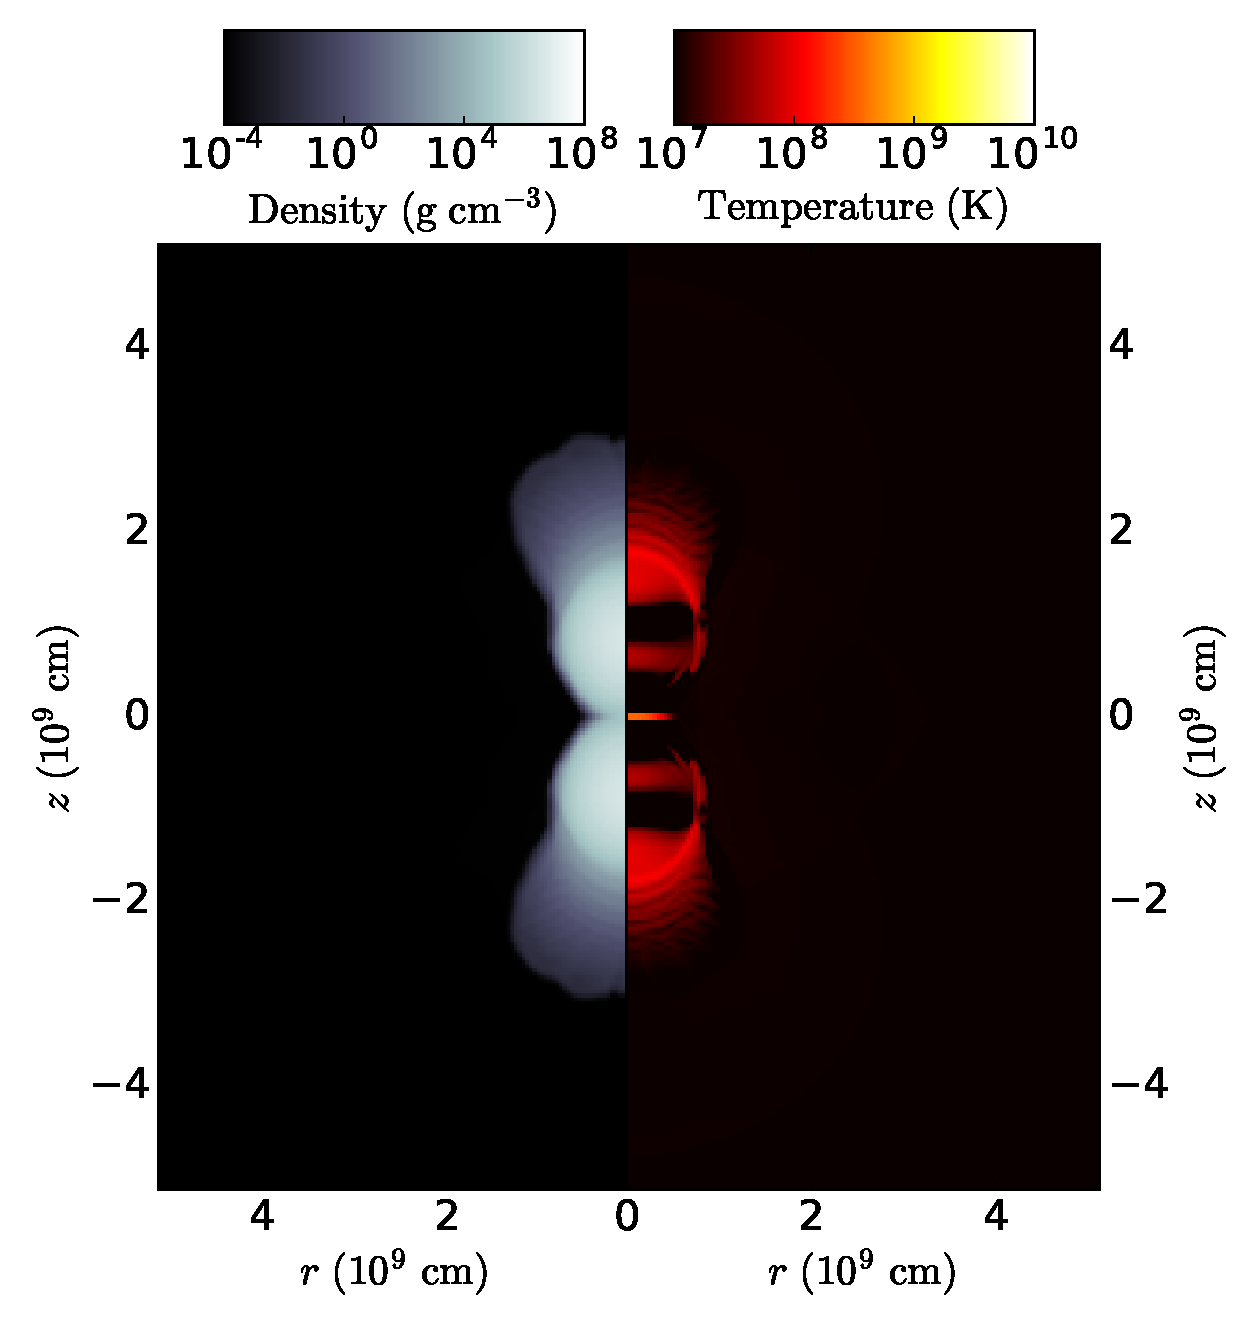
\includegraphics[scale=0.8]{{{plots/rho_T_slice_center_tagging_r1_t_5.01}}}
  \caption[2D collision at initial contact]
          {Temperature $T$ and density $\rho$ for the 2D collision as the
           WDs make initial contact. The domain is mirrored with respect to
           the $r = 0$ symmetry plane for visual purposes; the actual simulation
           domain is only the size of one of the two half-planes.
           \label{fig:initial_collision_state}
          }
\end{figure}


\clearpage
\subsection{Analysis}
\label{sec:analysis}

We track a number of diagnostic quantities at the end of coarse grid timesteps. 
For all simulations, we record the total energy (including the breakdown into
its components: kinetic, internal, gravitational potential, and rotation; we note
that for the diagnostics we actually use $(\rho E)$ for calculation of the total energy,
rather than explicitly calculating the sum of kinetic and internal, as this is
the quantity that should be explicitly conserved), 
the total angular momentum, and the center of mass of the system. 
We also separately record diagnostic 
information about the stars. Our strategy for tracking their 
locations is as follows: at the beginning of the calculation, we store the 
physical center of mass $\mathbf{x}_{c}$ of the stars as determined 
by Kepler's third law. We also store the velocity $\mathbf{v}_{c}$ 
of the stars. Then, at each new time step we make a preliminary guess for their 
location by updating the location using the old velocity, 
$\mathbf{x}_{c} \rightarrow \mathbf{x}_{c} + \mathbf{v}_{c} \Delta t$.
We then refine our guess for the location and velocity of each star by computing a
location-weighted sum of the mass and velocity over the computational domain. 
To do this, we need a cutoff for determining what counts as part of the primary 
and what counts as part of the secondary. We use a simple criterion: the star
that a zone ``belongs'' to is the one that exerts a larger magnitude
gravitational force on that zone (as computed using the tentative data
for that star's mass and radius). From this we obtain the corrected mass
of each star as well as its location and velocity. Once we have the new centers of mass,
we compute the effective radius of each star at various density cutoffs. This involves 
computing the volume $V$ of all zones that belong to the star (in the sense described above) 
whose density is greater than the cutoff. We then compute $r_{\text{eff}} = (3V/4\pi)^{1/3}.$

When we do simulations with adaptive-mesh refinement, there are multiple levels of refinement 
that contribute to a global integral. To deal with this we employ a ``mask'' which zeros out 
the data in a zone on a given level if there is a refined region overlying that zone.



\subsubsection{Gravitational Waves}
\label{sec:gravitational_waves}

A final diagnostic quantity we consider is the gravitational wave emission by the 
binary system. White dwarfs are not strongly affected by general relativistic effects;
the orbital motions are much slower than the speed of light, and the relativity parameter 
$GM / c^2 R$, which measures the ratio of the Schwarzschild radius of a mass $M$ to the actual 
radius $R$ of the object, is much less than unity for a white dwarf. Thus at any given time the 
relativistic effects are negligible compared to the Newtonian gravity and so we do not 
directly include relativistic effects in computing the dynamical evolution of the system.
A white dwarf binary system does emit gravitational waves during its evolution; this energy loss 
is what drives the initial inspiral over very long timescales for isolated binary systems, and
contributes to the orbital decay for hierarchical triple systems. Eventually it will drive the system 
to become dynamically unstable due to the Newtonian tidal forces alone, though once that period begins, 
the gravitational energy loss is inconsequential in affecting the dynamical evolution of the system. 
The frequency of the gravitational waves emitted by the white dwarf binary 
is similar to the frequency of the orbital motion, which is in the range 
10-100 mHz for our problem. This is well outside the range of currently existing 
gravitational wave detectors but is very well suited for proposed space-based detectors such as eLISA \citep{eLISA}.

We follow the prescription of \citet{blanchet:1990} for computing a gravitational wave 
signal for our simulation. At distances far from the 
gravitational wave source, we need only consider the leading term in the gravitational 
wave signal:
\begin{equation}
  h^{TT}_{ij}(t,\mathbf{x}) = \frac{2G}{c^4 r}P_{ijkl}(\mathbf{n}) \ddot{Q}_{kl}(t - r/c).
\end{equation}
$h$ is the perturbation to the spacetime metric and is commonly called the \textit{strain}; 
for laser interferometers, it measures the relative change in the distance between mirrors. 
The ``TT'' superscript indicates that we work in the commonly used tranverse-traceless gauge.
This strain is measured at time $t$ and position $\mathbf{x}$ relative to the binary system.
$r\equiv |\mathbf{x}|$ is the distance from the observer to the binary system. The unit vector 
$\mathbf{n} \equiv \mathbf{x} / r$ then measures the direction of the outgoing wave with 
respect to the observer, and $P_{ijkl}(\mathbf{n})$ is an operator that projects a tensor 
onto the direction orthogonal to $\mathbf{n}$:
\begin{align}
  P_{ijkl}(\mathbf{n}) &= \left(\delta_{ik} - n_i n_k\right)\left(\delta_{jl} - n_j n_l\right) \notag \\
                      &- \frac{1}{2}\left(\delta_{ij} - n_i n_j\right)\left( \delta_{kl} - n_k n_l\right).
\end{align}
$Q_{kl}$ is the quadrupole moment tensor:
\begin{equation}
  Q_{kl} = \int dV \rho \left(x_k x_l - \frac{1}{3}\delta_{kl} \mathbf{x}^2\right).
\end{equation}
The argument $(t - r/c)$ indicates that to get the strain at time $t$ we evaluate the second derivative of the 
quadrupole moment at the retarded time $t - r/c$. In practice the retarded time is simply the simulation time
and the observer would see the gravitational waves after a time delay of order $r/c$.

Therefore the primary component of the calculation is the evaluation of the second time derivative of $Q_{kl}$.
Explicitly constructing a discretized form of this derivative, using the current state and the state at 
previous times, is undesirable because of the inherent imprecision (its accuracy depends on the size of the timestep),
in addition to the logistical challenges that may be implied by saving and using previous simulation states. 
\citet{blanchet:1990} provide a prescription for this time derivative purely in terms of the state at a given time:
\begin{equation}
  \ddot{Q}_{kl} = \text{STF}\left\{2\int dV \rho (v_k v_l + x_k g_l)\right\}.
\end{equation}
The symmetric trace-free (STF) operator is defined as:
\begin{equation}
  \text{STF}\left\{A_{ij}\right\} = \frac{1}{2}A_{ij} + \frac{1}{2}A_{ji} - \frac{1}{3} \delta_{ij} \sum_{k}A_{kk}.
\end{equation}

The strategy is then as follows. At the end of the coarse timestep, we first calculate $\ddot{Q}_{kl}$
using an integral over the domain. This quantity is independent of the observer. If we 
are using a rotating reference frame, we first convert velocities and positions back to the inertial 
frame before evaluating the integral. Then, 
we pick an observing location $\mathbf{x}$ relative to the domain, evaluate the projection operator, 
and then perform the relevant tensor contraction to determine the strain tensor. We can 
repeat this process for any number of observing locations at minimal cost, since the quadruple tensor 
only needs to be calculated once. Gravitational waves only excite modes orthogonal to their 
direction of travel. These are the ``plus'' and ``cross'' modes, $h_+$ and $h_\times$, named after 
the types of spatial distortions they exhibit. We calculate the signal at a distance $r$ along 
the $x$, $y$ and $z$ axes. For the latter, as an example, $h_{+} = h_{11} = -h_{22} \propto (\ddot{Q}_{11} - \ddot{Q}_{22})/2$ and 
$h_{\times} = h_{12} = h_{21} \propto \ddot{Q}_{12}$. All other entries vanish. By default we take $r = 10$ kpc; 
as shown by \citet{loren-aguilar:2005}, this is a typical distance scale over which an 
experiment such as LISA could detect a coalescing binary white dwarf system. 
The strain at any other distance is easily calculated and goes as the inverse of the distance.



\newpage
\section{Verification Tests}
\label{sec:verification}

White dwarf merger simulations face a number of numerical difficulties,
including the typical issues that make any numerical hydrodynamics simulation
challenging, but also a number of difficulties that are
not present in single-degenerate Type Ia and core-collapse supernova
simulations.  Thus while the behavior of \castro\ for many standard hydrodynamics
test problems was detailed in the original code paper \citep{castro}, and the code
is regularly subjected to a battery of test problems that ensure it gives reasonable
results, the usual suite of problems needs to be complemented by a set of tests
that exercise the features unique to binary star systems. In \autoref{sec:gravity},
we gave examples of how the gravity solver can affect such a system, for example
through the boundary conditions on the potential and the way the gravitational source
term is added to the hydrodynamics update. There are also hydrodynamical issues that
are specific to the case where large amounts of material move at significant speeds
across the grid, and the merger process is just such a case. This bulk motion presents
an opportunity for advection errors to build up, and is only partially mitigated by
evolving the white dwarfs in a co-rotating frame. It is therefore important to be
aware of the behavior of the code in such circumstances.

Our focus here is on a subset of problems that highlight the special difficulties
introduced in merger simulations. These problems couple the hydrodynamics, gravity and
equation of state modules. We observe that while in most non-trivial
three-dimensional problems this creates a complexity that makes it
impossible to determine exact analytical solutions, it is
straightforward to devise problems for which certain global properties
should obey simple, expected behaviors. Where possible, these should
be quantified and a convergence study performed; where not, we should at least
be able to run the test and see whether the results make sense given what
we know about the properties of the system. We should also at least be able
to see whether the results converge with numerical resolution (even if we cannot
see whether this convergence is to the correct answer for the problem).
This is the focus of the current section.

\subsection{Maintaining Hydrostatic Equilibrium}
\label{sec:HSE}

In \autoref{sec:initial_models} we describe the process by which
we generate initial stellar models. While the 1D models are in
hydrostatic equilibrium to within a small error, interpolation onto
the 3D Cartesian grid will introduce perturbations into the solution
\citep{zingale:2002}. Although we ensure that the initial models are
generated with the same equation of state and are at least as well resolved as
our finest grid, there is still be a hydrodynamical error associated
with the fact that the rectangular grid cannot faithfully represent a
spherical star. Additionally, the gravitational potential obtained by
the multigrid solver will differ slightly from the one assumed by the
initial model, and the operator splitting between the gravity and
hydrodynamics should also result in small errors. As a result, we
expect that the star will oscillate slightly about an equilibrium
point, but that the amplitude of this oscillation should decrease with
increasing resolution.

\begin{figure}[h!]
  \centering
  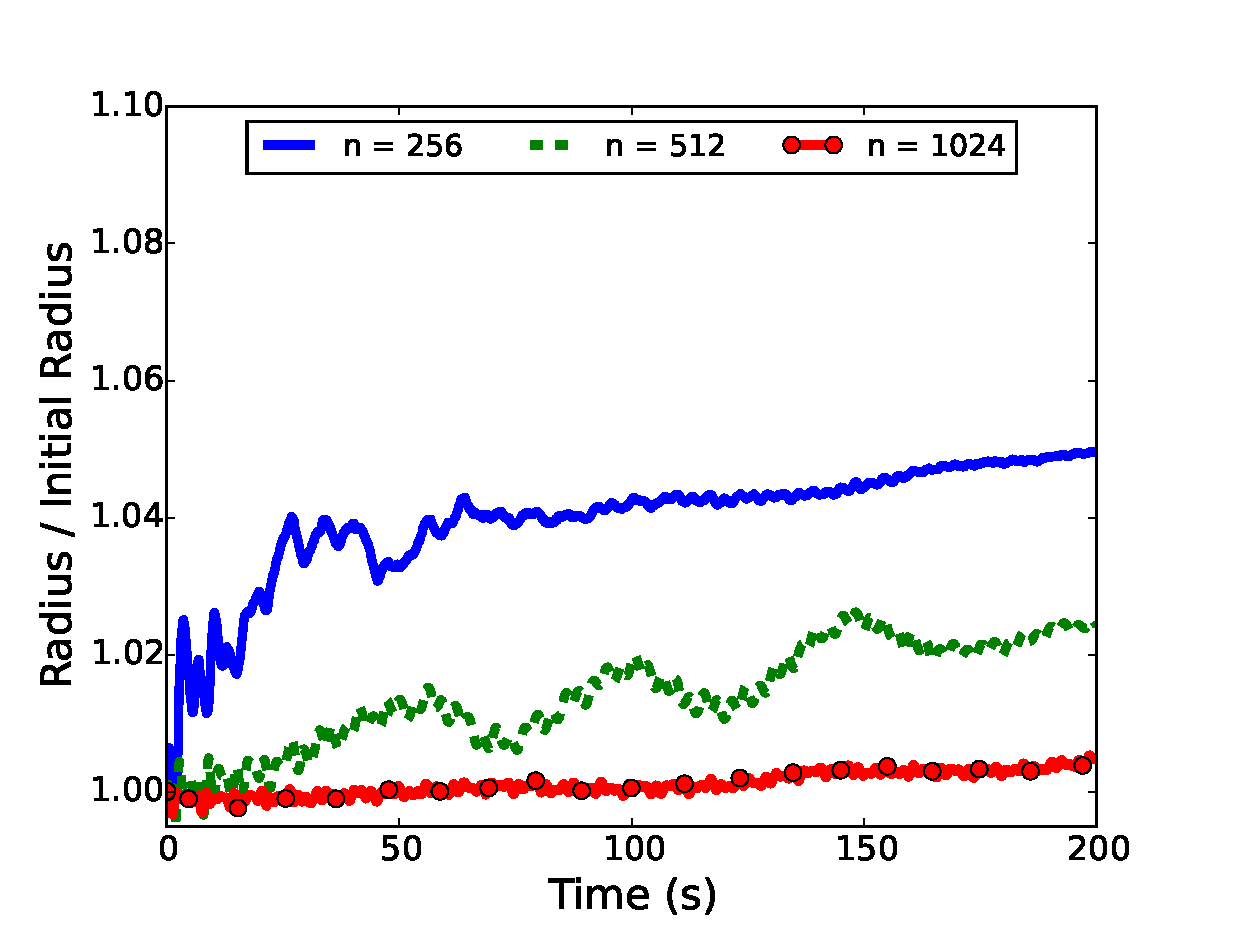
\includegraphics[scale=0.8,trim=0.15in 0.0in 0.55in 0.5in,clip]{plots/single_star_static_1e3_radius}
  \caption[Effective radius evolution of a static white dwarf]
          {Time evolution of the effective radius of a $0.9 \msolar$ 
           white dwarf, seeded onto the grid using a one-dimensional hydrostatic
           model and evolved without further relaxation. The lines represent 
           different number of zones per spatial dimension; when this number is 
           greater than 256, it represents an effective resolution obtained 
           using AMR levels that cover the star. The radius is determined 
           using the volume of the grid that has a density greater than $10^3\ \text{g cm}^{-3}.$
           \label{fig:single_star_static_radius}}
\end{figure}

This problem was studied in the first \castro\ paper, but is worth
revisiting here. A single star explosion simulation may only last a
couple of seconds, and the \castro\ paper studied the behavior of the
star after one second of evolution. However, the dynamical timescale
of a typical carbon-oxygen white dwarf is on the order of 1--10
seconds. Additionally, a binary orbit is typically on the order of
10--100 seconds when a merger simulation starts, and with equilibrium
initial conditions the system may survive for tens of orbits before
the secondary is disrupted. When this does happen, we want to be
confident that it was because of the dynamics of the merger process
and not because of an instability in an individual star. Our goal here
is thus to install a single star onto our three-dimensional
coordinate grid and evolve it for a period of time long enough to
assess whether the star is truly stable, and to probe how the size of
deviation from equilibrium is affected by grid resolution.

We loaded a single star of mass $0.9\ \msolar$ onto the grid at the
origin, and evolved it for 200 seconds. Our diagnostic of choice is
the effective radius of the star, determined by the volume of the grid
that has a density greater than $10^3\ \text{g cm}^{-3}$ (see
\autoref{sec:software} for details on this measure). This choice
of density is intended to mark a reasonable outer edge to the star
that is not immediately susceptible to the numerical errors prevalent
near the physical edge of the star.
\autoref{fig:single_star_static_radius} shows our results at various
resolutions.  As expected, the star quickly approaches an equilibrium
size that is different (and in this case larger) than the
one-dimensional model, though the magnitude of this change becomes
smaller with resolution. The star is only approximately in equilibrium 
by this measure when the coarse grid of $256^3$ zones has a level of 
refinement that jumps by a factor of four. Even then there is a slight uptick
in the size toward the end, implying that the numerical stability is
not guaranteed for arbitrarily long timescales. For another view, we 
consider the kinetic energy on the grid, in \autoref{fig:single_star_static_ke}. 
This is a more holistic measure that weights the contribution by the density. 
At the end of the simulation the kinetic energy is not lower at the highest 
resolution than at the lower resolutions. This result suggests
that when constructing the equilibrium initial models that will form the
basis of later calculations, we should carefully monitor the evolution
of the stars when applying any artificial damping to cause the
merger, to ensure that the merger is due to this applied force and not
the intrinsic numerical instability of the stars.
\begin{figure}[h!]
  \centering
  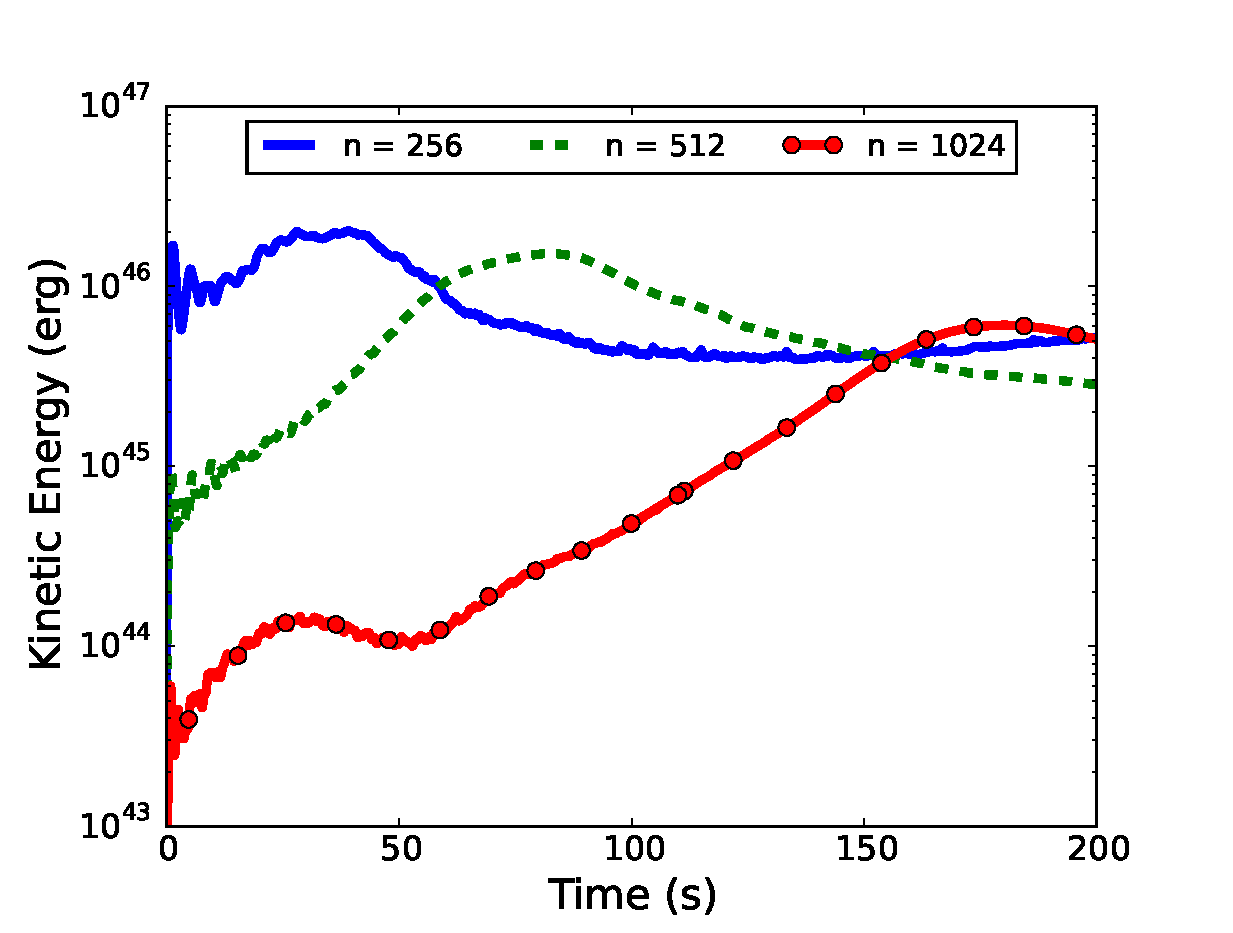
\includegraphics[scale=0.80,trim=0.1in 0.0in 0.55in 0.45in,clip]{plots/single_star_static_ke}
  \caption[Kinetic energy evolution of static white dwarf]
          {Time evolution of the kinetic energy of a $0.9\, \msolar$ 
           white dwarf. The lines have the same meaning as in \autoref{fig:single_star_static_radius}.
           \label{fig:single_star_static_ke}}
\end{figure}

\clearpage
\subsection{Gravitational Free Fall}
\label{sec:Gravitational Free Fall}

A simple dynamical test to verify the coupling between the gravity and hydrodynamics in \castro\ is
the case of gravitational free fall. We place two stars on the grid 
in the manner of \autoref{sec:software}. The distance $a$ between 
them corresponds to a chosen orbital period $T$, consistent with the total
system mass $M$, but we disable the rotational source terms so that 
the stars start at rest in an inertial reference frame. 
Thus the stars will simply begin moving toward each other.
As long as the stars remain approximately spherical, the stars can be 
treated as point masses (this approximation only seriously breaks down after the stars
have come into contact). In dimensionless units where $r \to r / a$ and 
$t \to 2\sqrt{2}\pi t / T$, the simple free fall equation of motion governing the
distance $r$ between their centers of mass takes the form:
\begin{equation}
  \ddot{r}(t) = - \frac{1}{2r^2}.
\end{equation}
It is possible to derive a closed-form solution for the evolution time
as a function of separation by starting with the integral formulation,
\begin{equation}
  t(r) = \int_{1}^{r} \frac{dr}{v(r)}.
\end{equation}
The velocity $v$ (in dimensionless units) can be found by noting that 
$\ddot{r} = v\, dv / dr$ and then separating and integrating the equation 
of motion. This yields 
\begin{equation}
  v(r) = \sqrt{\left(\frac{1}{r} - 1\right)}.
\end{equation}
For our problem $0 < r \leq 1$, so this is always valid. Integrating, we find
\begin{equation}
  t(r) = \text{arccos}\left(\sqrt{r}\right) + \sqrt{r \left(1 - r\right)}. \label{analyticalFreeFall}
\end{equation}
so that the point of contact would occur at $t = 1$. We actually stop the simulation
at $t = 0.9$, which is when the effects from the extended sizes of the stars
starts to become important. The results of our simulation for our default $256^3$ zone 
uniform grid are shown in \autoref{fig:freefall}. They show excellent agreement
between the analytical solution and the simulation results.

\begin{figure}[h!]
  \centering
  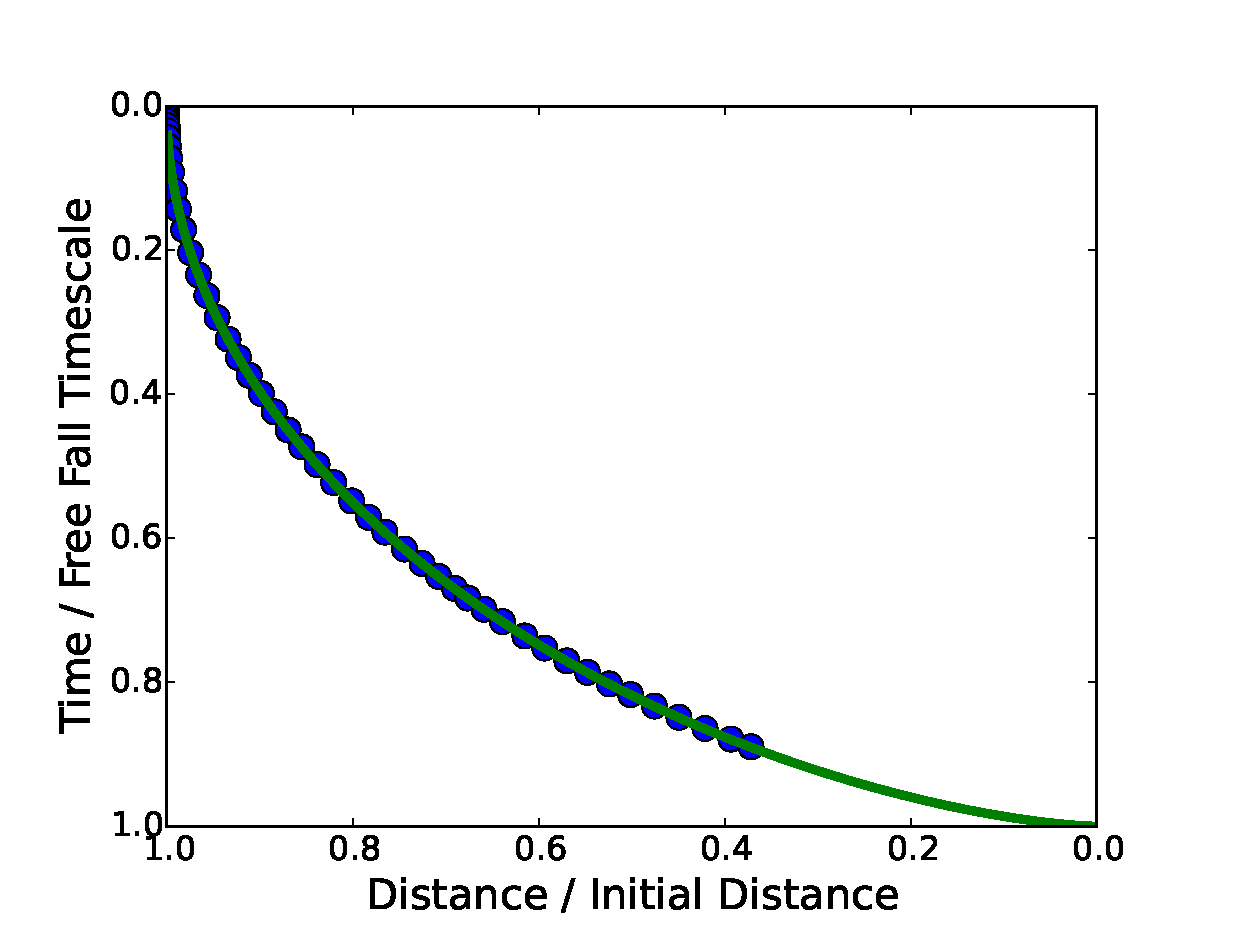
\includegraphics[scale=0.80,trim=0.3in 0.0in 0.8in 0.5in,clip]{plots/freefall}
  \caption[Gravitational free-fall test]
          {Time evolution of two initially stationary white dwarfs,
           mutually attracted to each other by the gravitational force. The
           horizontal axis gives the separation of the white dwarfs, scaled
           to the initial separation, and the vertical axis gives the elapsed
           time of the simulation, scaled to the time it would take two point masses
           to collide. The solid curve shows the analytical result,
           calculated from Newtonian mechanics, and the circles show the
           samples from the time evolution with \castro. For visual clarity, we 
           show only a small fraction of the timesteps.\label{fig:freefall}}
\end{figure}

\subsection{Galilean Invariance}
\label{sec:galileo}

It is often stated in the literature that Eulerian methods for
hydrodynamics with grids fixed in space do not obey the Galilean
invariance of the underlying Euler equations, so that simulations
moving at a uniform bulk velocity appear different than an
equivalent stationary simulation (e.g. \cite{arepo}). If true, we need to understand 
the importance of this effect when deciding whether to trust the 
output of a code like \castro\ when applied for merger problems.
Recently, concern for the issue of Galilean invariance has come up in two ways which are of note for us 
in the present study. We explain these situations and display 
the results of tests we have run to determine whether this 
actually is a significant concern for our study.

\citet{arepo} (hereafter, S10) performed a Kelvin-Helmholtz instability test and showed
that (at low resolution) a fixed-grid code failed to develop the
expected fluid instability when the whole fluid was moving at a
strongly supersonic uniform velocity. (See also \citet{wadsley:2008}, 
who used the \flash\ code to simulate a hot bubble subject to mixing 
by the Kelvin-Helmholtz instability, and also found that the mixing was affected by a 
uniform bulk velocity.) This contrasted with the results
of the moving-mesh code \arepo\ being presented in that study, which
demonstrated Galilean invariance even at large bulk velocities. 
Inability to correctly model the Kelvin-Helmholtz instability would 
have important consequences for how much we can trust the ability of 
\castro\ to test the violent merger progenitor model, where a detonation 
arises in the low-density material at the stellar surface. Shearing between 
the material flowing out of the secondary and material near the 
surface of the primary may trigger fluid
instabilities that play an important role in the evolution of that
gas, which is the site of the initial detonation in the prompt
explosion model. \citet{guillochon:2010} showed for their simulation
that Kelvin-Helmholtz instabilities produced this way may raise the
temperature of the accreting material enough to ignite a
detonation. Therefore if we are not correctly reproducing the
characteristics of the Kelvin-Helmholtz instability in the case where
there is significant mass motion on the grid, we cannot be confident
that a detonation (or lack thereof) is not numerically
seeded. 

\citet{robertson:2010} (hereafter, R10) observe that violation of Galilean
invariance of simulation results for the Euler equations occurs 
because of truncation error in the discretization of the fluid
equations. This takes the form of a numerical diffusion term which is
dependent on velocity (and also resolution). The advantage of a
moving-mesh code is that the mesh everywhere moves with the local flow
velocity, which substantially reduces the numerical
diffusion. R10 argue that the differences seen
between the moving-mesh and fixed-grid code are caused by the
interaction of this numerical diffusion with small-scale instabilities
(that may be physical or numerical) which couple with and
fundamentally alter the large-scale modes. Small-scale instabilities
are seeded by the choice of a sharp initial discontinuity between the 
fluids in the problem posed by S10. Crucially though,
R10 point out that this problem does not
converge with resolution (because the initial perturbation is too sharp 
and seeds numerical noise at the grid resolution level) 
and so it is not possible to know the correct
behavior of this problem. As such, we do not know whether the
small-scale modes found in \arepo\ are real, and the problem is not
useful in formally discriminating between methodologies. They instead
propose an alternate test with a smoother initial contact. This
converges to the same solution qualitatively in both the stationary
and bulk velocity cases, indicating that the code does generally
maintain Galilean invariance (to some specified error that depends on
resolution and the uniform flow speed).  We will see whether we can
reproduce this result.

A related question is whether our code reliably simulates the bulk
motion of the stars across the grid, and whether such bulk motion
affects the stability of the star. This concern is prompted by the
study of \cite{tasker:2008}, who studied the effect of uniform
translation on the stability of a spherically symmetric model for a
galaxy cluster. They compared the radial profile of the cluster at
initialization and after a period of time evolution. Using \flash\ and
\enzo, they found that a static cluster retains its shape at high
enough resolution, while uniform translation of the cluster causes
mixing of the core material due to numerical diffusion which results
in an underestimation of the core's true density. The SPH codes they
used did a better job maintaining the core density. We will perform a
variant of this test using white dwarf models.

\subsubsection{Kelvin-Helmholtz Instability}
\label{sec:khi}

Following \cite{robertson:2010}, we set up a Kelvin-Helmholtz test in
the following way. The problem domain runs from 0 to 1 in both the $x$
and $y$ directions. This is a two-dimensional test, so we run
\castro\ in 2D mainly to avoid extra computational expense; in 3D, it 
would merely involve replicating the problem in the $z$ direction.
The problem involves a fluid slab of density $\rho_2 = 2.0$ traveling rightward in the
$x$-direction at velocity $v_2 = 0.5$, sandwiched by a fluid of
density $\rho_1 = 1.0$ traveling leftward at velocity $v_1 =
-0.5$. The density gradient is in the $y$ direction, so this creates a
velocity shear along the interface between the fluids. The density and
velocity distribution on the computational domain are given by:

\begin{figure}[h!]
  \centering
  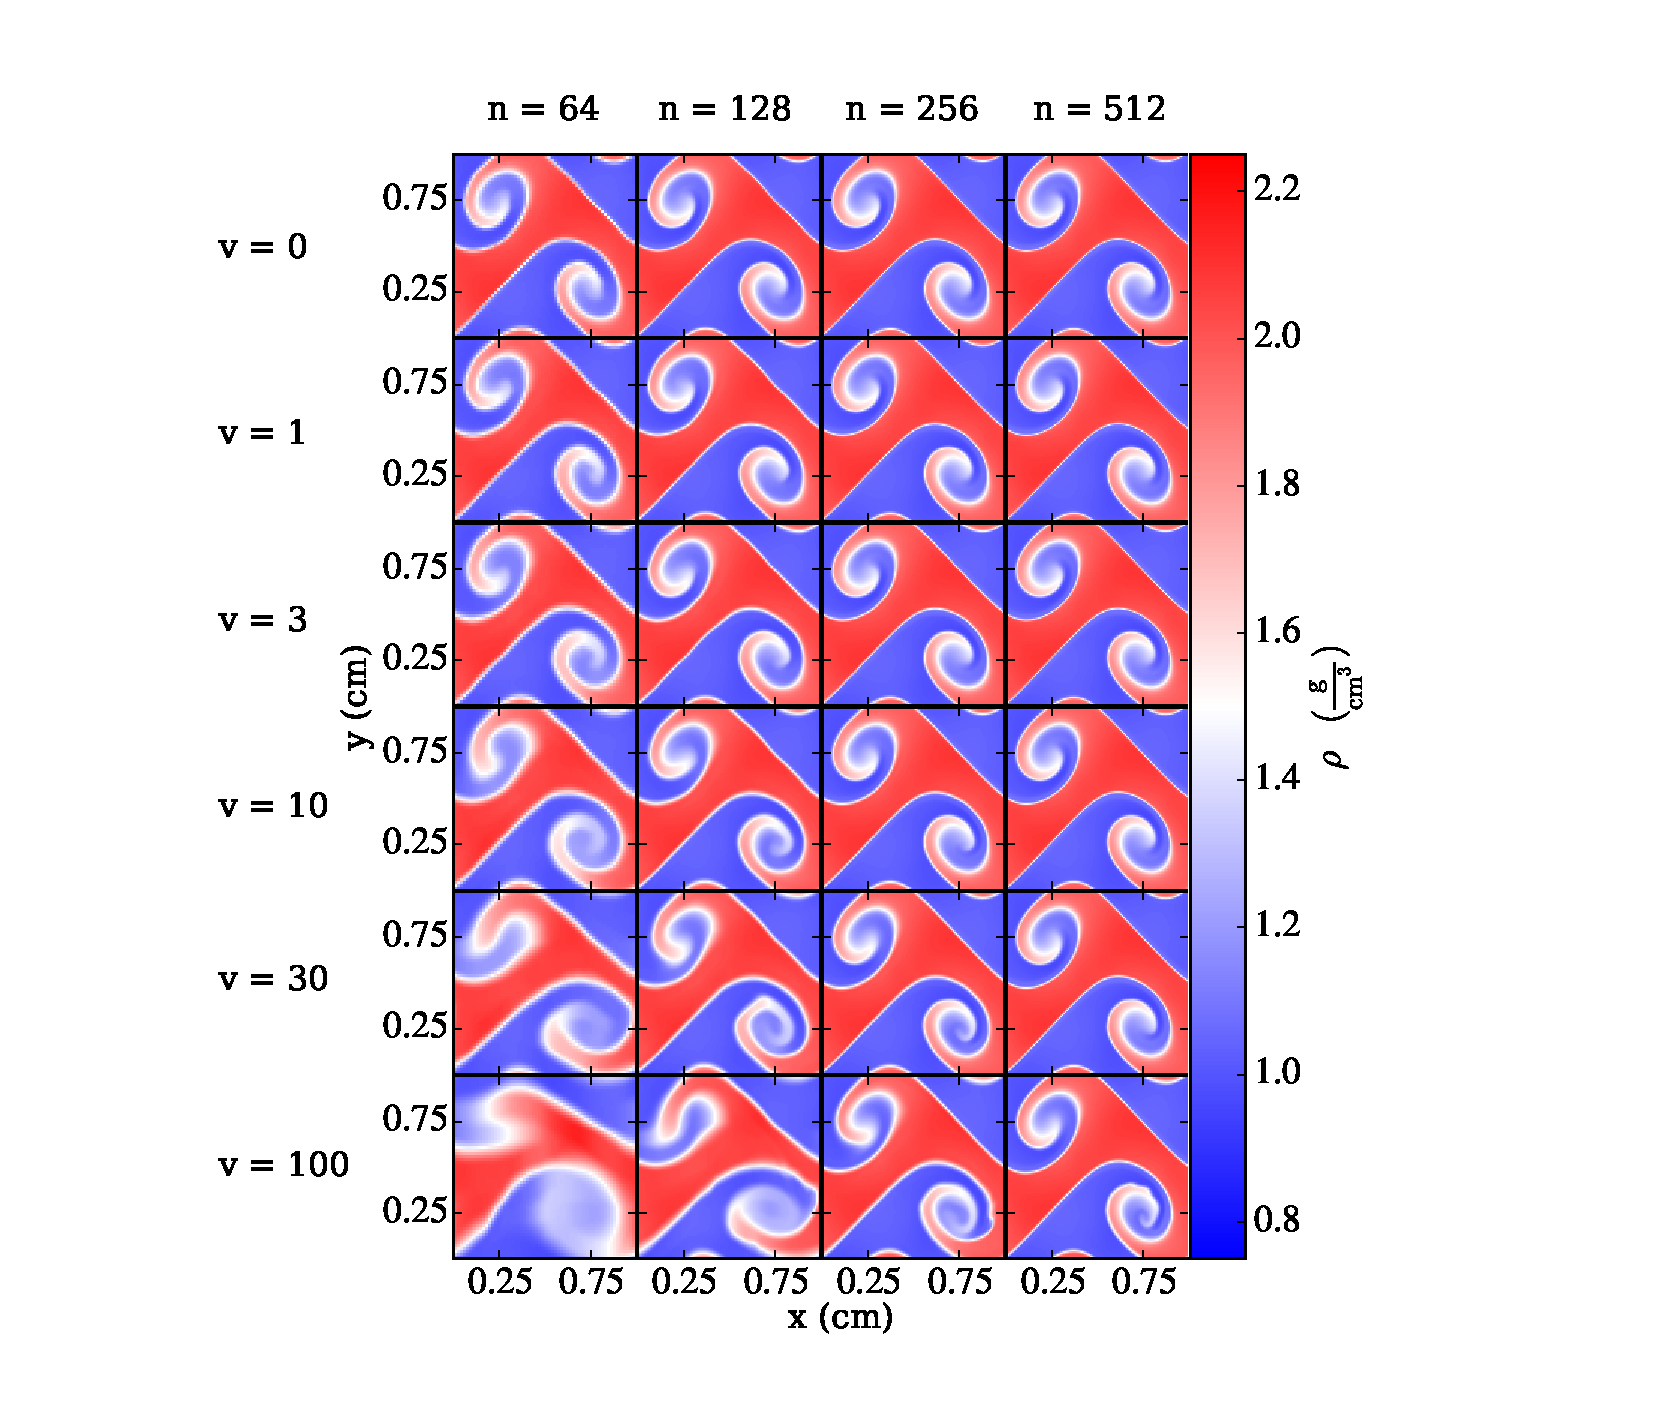
\includegraphics[trim=0.75in 0.45in 0.85in 0.5in, clip, scale = 0.75]{{{plots/kh_t2.0_p2_low_res_collage}}}
  \caption[Kelvin-Helmholtz instability and bulk velocity (Robertson et al.)]
          {2D Kelvin-Helmholtz instability test at $t = 2.0$ for the initial 
           conditions given by \autoref{eq:kh_ic_b_ramp} and \autoref{eq:kh_ic_b}. 
           The rows each represent a different bulk fluid velocity $v$ and 
           the columns each represent a grid resolution $n$ (the number of 
           zones per spatial dimension). The highest velocity simulation, 
           $v=100$, corresponds to approximately Mach 70. Compare to 
           Robertson et al. (2010), Figure 7. \label{fig:kh_p2}}
\end{figure}

\begin{align}
  \rho &= \rho_1 + R(y)\left[\rho_2 - \rho_1\right] \\
  v_x  &= v_1 + R(y)\left[v_2 - v_1\right] \\
  v_y  &= v_{\text{bulk}} + v^\prime
\end{align}

Here $R(y)$ is a ramp function that describes the transition between
the two fluids, while $v_{\text{bulk}}$ is the bulk motion of the
fluid in the $y$ direction and $v^\prime$ is the velocity perturbation
that seeds the instability. The problem is established for two
sets of initial conditions (ICs), which we follow
R10 in calling ICs A and B. They differ in
their ramp function ($R_A$ and $R_B$ respectively), as well as the
initial perturbation ($v^\prime_A$ and $v^\prime_B$ respectively), and
the frequency of the perturbation ($n_A = 4$ and $n_B = 2$):
\begin{align}
  R_A &= \begin{cases} 0 & |y - 0.5| > 0.25 \\ 1 & |y - 0.5| < 0.25 \end{cases} \label{eq:kh_ic_a_ramp}\\
  R_B &= \Big\{\left[1 + e^{-2(y-0.25)/\Delta y}\right]\left[1 + e^{2(y-0.75)/\Delta y}\right]\Big\}^{-1} \label{eq:kh_ic_b_ramp}
\end{align}
\begin{align}
  v^\prime_A &= w_0\, \text{sin}\left(n_A\, \pi\, x\right) \left\{e^{-(y-0.25)^2 / 2\sigma^2} + e^{-(y-0.75)^2/2\sigma^2}\right\} \label{eq:kh_ic_a}\\
  v^\prime_B &= w_0\, \text{sin}\left(n_B\, \pi\, x\right). \label{eq:kh_ic_b}
\end{align}
Here $w_0 = 0.1$ is the scale of the velocity perturbation, $\sigma =
0.05/\sqrt{2}$ controls the width of the Gaussian for IC A, and
$\Delta y = 0.05$ is the transition distance scale for the smooth ramp of IC
B. The pressure everywhere is set to $p = 2.5$, and we run this with a
gamma-law equation of state set to $\gamma = 5/3$. Plotfiles are
generated every 0.05 seconds, and the problem is run until $t = 2$.

\begin{figure}[h!]
  \centering
  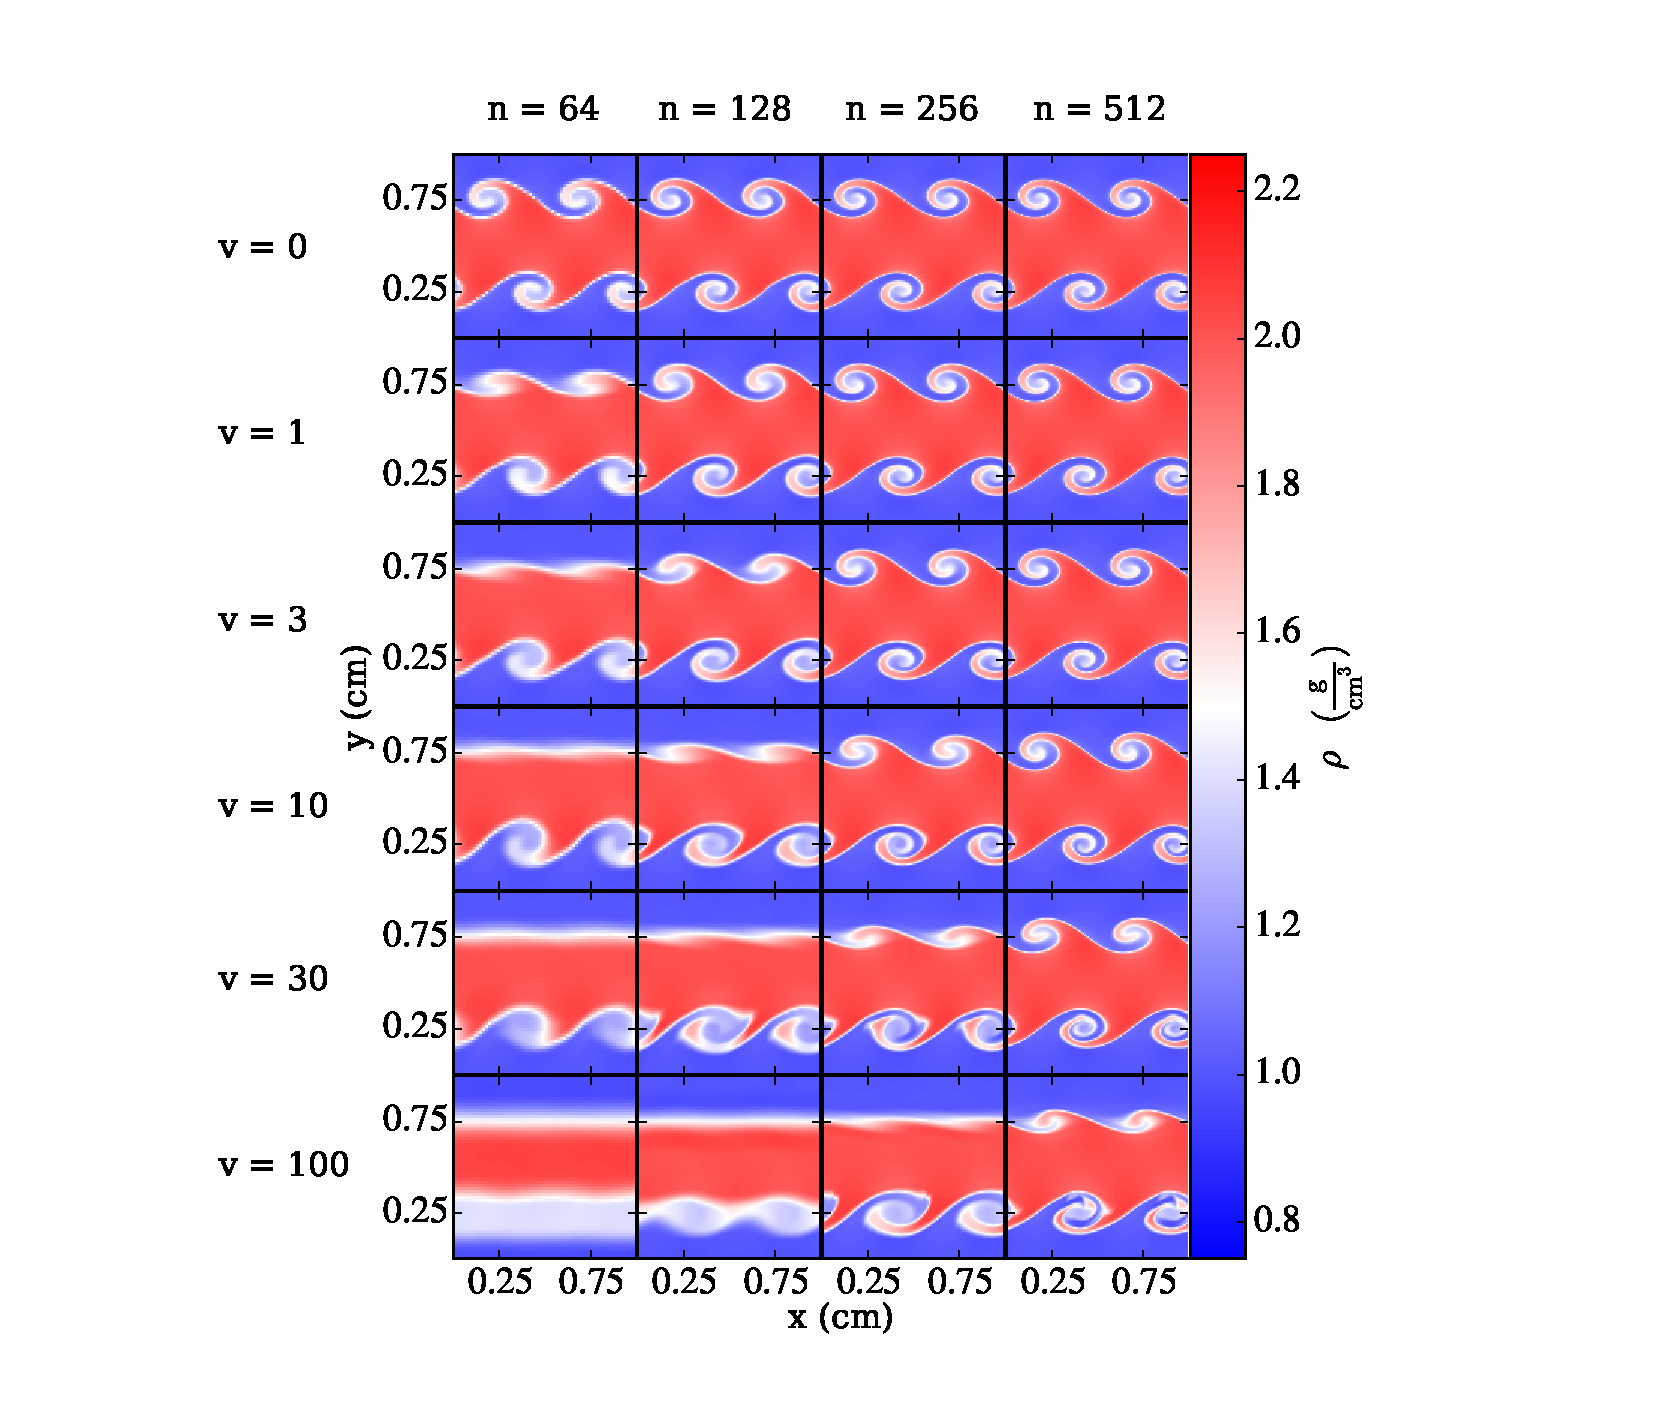
\includegraphics[trim=0.75in 0.45in 0.85in 0.5in, clip, scale = 0.75]{{{plots/kh_t2.0_p3_low_res_collage}}}
  \caption[Kelvin-Helmholtz instability and bulk velocity (McNally et al.)]
          {2D Kelvin-Helmholtz instability test at $t = 2.0$ for the initial 
           conditions given by \autoref{eq:kh_p3_rho} through \autoref{eq:kh_p3_vy},
           which come from McNally et al. (2012).
           The meaning of the rows and columns is the same as in \autoref{fig:kh_p2}.
           \label{fig:kh_p3}}
\end{figure}

We run the problem for $v_\text{bulk} = [0, 1, 3, 10, 30, 100]$, and
for each set of initial conditions run the problem at resolutions of
$64^2$, $128^2$, $256^2$, $512^2$. For context, in these units the 
sound speed is $c\approx 0.7$. In addition, for each initial
condition we run simulations at the higher resolutions of $1024^2$,
$2048^2$, and $4096^2$ for the stationary problem only. These serve 
as a reference solution to gauge the extent to which the bulk flow 
affects the development of the fluid instability, and to determine 
if the problem is numerically converged.

We find the same result as R10 for IC A, which is equivalent to the 
test proposed by S10: at low resolutions and high bulk velocity, the 
Kelvin-Helmholtz instability completely fails to develop. Furthermore 
the problem does not converge even qualitatively at the highest 
resolutions we used. Our results are very similar to Figure 3 of 
R10 so we do not show them here. For IC B, our results can be seen 
for the normal resolutions and all velocities in \autoref{fig:kh_p2}.
At low resolutions and very large bulk velocities, the fluid 
does get significantly disrupted by numerical error. This 
effect quickly converges away with resolution and qualitatively 
at $512^2$ resolution the solution is nearly identical to the stationary 
$v=0$ problem. We agree with R10 that this problem does converge 
with resolution and is not subject to numerically-seeded secondary 
instabilities at the stopping time. This is evident even at low resolutions
by examining the first row of \autoref{fig:kh_p2}.

\begin{figure}[h!]
  \centering
  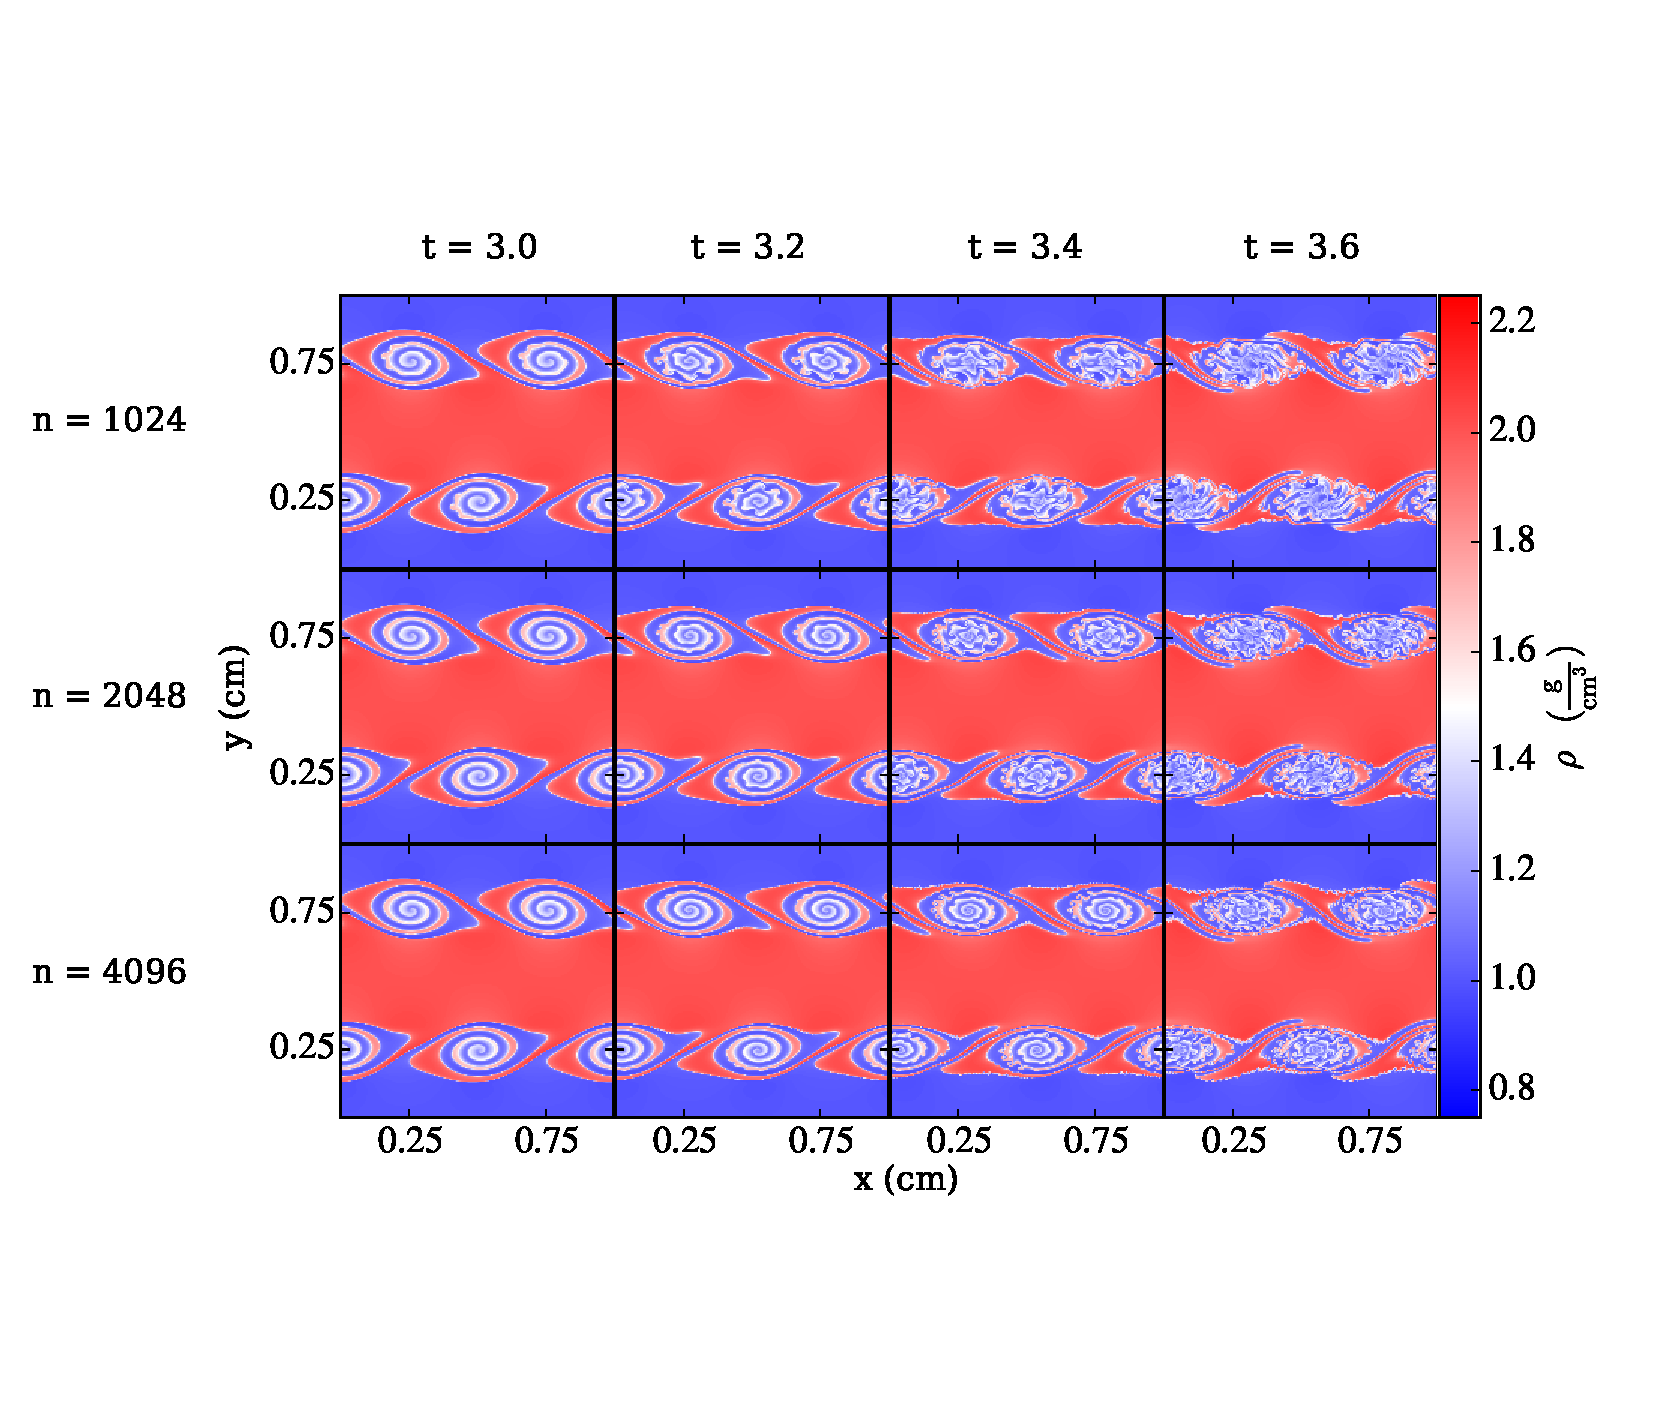
\includegraphics[trim = 0in 1.25in 0.25in 1.25in, clip, scale=0.6]{{{plots/kh_p3_high_res_collage}}}
  \caption[High-resolution Kelvin-Helmholtz instability]
          {Time series of the Kelvin-Helmholtz problem proposed by McNally et al. (2012)
           as the simulation is just starting to go non-linear. The rows represent resolution, 
           where $n$ is the number of grid cells per spatial dimension, and the columns are 
           different snapshots in time.\label{fig:kh_p3_high_res}}
\end{figure}

\citet{mcnally:2012} published another Kelvin-Helmholtz problem that 
is well-posed in the sense that it converges with resolution and 
is not subject to uncontrollable numerical instabilities. Though they 
were not explicitly interested in the question of Galilean invariance, 
we visit that issue here to see what can be learned. The initial 
conditions for this problem are:
\begin{align}
  \rho &= \begin{dcases} \rho_1 - \rho_m e^{(y-0.25)/\Delta y} & 0.25 > y \geq 0 \\ 
                         \rho_2 + \rho_m e^{(0.25-y)/\Delta y} & 0.5 > y \geq 0.25 \\
                         \rho_2 + \rho_m e^{(y-0.75)/\Delta y} & 0.75 > y \geq 0.5 \\
                         \rho_1 - \rho_m e^{(0.75-y)/\Delta y} & 1 > y \geq 0.75 \end{dcases} \label{eq:kh_p3_rho}
\end{align}
\begin{align}
  v_x &= \begin{dcases} v_1 - v_m e^{(y-0.25)/\Delta y} & 0.25 > y \geq 0 \\
                        v_2 + v_m e^{(0.25-y)/\Delta y} & 0.5 > y \geq 0.25 \\
                        v_2 + v_m e^{(y-0.75)/\Delta y} & 0.75 > y \geq 0.5 \\
                        v_1 - v_m e^{(0.75-y)/\Delta y} & 1 > y \geq 0.75 \end{dcases} \label{eq:kh_p3_vx} \\
  v_y &= w_0\, \text{sin}\left(4\pi x\right). \label{eq:kh_p3_vy}
\end{align}
Here $\Delta y = 0.025$, $w_0 = 0.01$, $v_m = (v_1 - v_2) / 2$, $\rho_m = (\rho_1 - \rho_2) / 2$, 
and the other symbols have the same meaning as above (this means the flow direction
is reversed compared to the original paper, so as to achieve consistency with the 
other simulations presented here). We run this problem at all the same resolutions 
and bulk velocities as the previous two problems. The results for the normal resolutions 
at $t = 2.0$ are displayed in \autoref{fig:kh_p3}. We see a similar pattern as for 
the test proposed by R10: as we get to higher flow speeds we need to have higher 
spatial resolution to compensate for the increased numerical diffusion. The 
qualitative accuracy is much lower for the highest bulk velocities for this problem
than for the previous problems. This is because the amplitude of the instability overall
is smaller than for the previous problems, at least by $t = 2.0$, so it is easier
for numerical diffusion at the shearing layer, caused by the high bulk velocities,
to completely wipe out the instability. Like \citet{robertson:2010} found for
their problem, we find for this problem that the convergence properties are not
substantially affected by altering the perturbation frequency -- the results
show the same qualitative pattern even if we halve this frequency.

\citet{hopkins:2015} performed this test as part of the testing of
their code GIZMO.  They showed the late-time evolution of this system,
when non-linear effects have taken over and significantly disrupted
the initial flow. At low resolution the tested grid algorithm
had failed to disrupt both for $v = 0$ and $v = 10$. We too ran this
problem until $t = 10$, and confirm that the Kelvin-Helmholtz
instability damps out at low resolution but goes strongly non-linear
and disrupts the flow at high resolution.  We strongly
emphasize the point that this does not objectively demonstrate a
deficiency in fixed-grid codes for this problem. We can only determine
the validity of a method when we have a trustworthy, converged
solution to compare to, and this is lacking for this problem at late
times. As observed by \citeauthor{mcnally:2012}, this lack of a solution is because the
secondary instabilities form for this problem when the whorls of the
Kelvin-Helmholtz tendrils stretch out and create gradients that
approach the grid resolution. This is prime breeding ground for
numerical noise. But because the nature of this noise depends on
the resolution, it is very different for simulations at different
resolutions. If these instabilities are seeded because of this
resolution-dependent noise and are not seeded instead in a controlled
manner such that they appear at the same time and location, then we
simply cannot draw any conclusions that bear on the question of
verification from this test at late times.
\autoref{fig:kh_p3_high_res} provides a sense of this by examining the
crucial time at which the transition from the linear to the non-linear
regime is occurring.  At all of these very high resolutions the
secondary instabilities develop, but they occur at different times and
have different spatial scales for each resolution.

We conclude that large bulk motions of fluid can have very significant effects 
on numerical calculations of shear mixing in fixed-grid codes, but that this effect 
diminishes with increasing resolution. As a result, we must be confident that we are 
sufficiently resolving the major mixing regions on the white dwarf surfaces,
specifically that the density gradients occur over spatial scales much larger
than the grid resolution. If we find instead that this mixing occurs near the
grid resolution scale, this will imply that we need to ramp up the resolution
in these regions using AMR. If this becomes too expensive, we would need to be
skeptical of any conclusions that could be drawn 
about the effect of the mixing on the nuclear burning.

\clearpage
\subsubsection{Moving Star}
\label{sec:moving_star}

To analyze the effects of velocity-dependent results for a stellar simulation, we repeated the
test of \autoref{sec:HSE} with a bulk velocity on the grid. We chose a
velocity of $2.56 \times 10^{8}\ \text{cm s}^{-1}$. For context, this is 
comparable to the orbital velocities of the stars in \autoref{sec:kepler}, and the Mach
number is of order unity in the stellar core at this speed.  This test
was inspired by \citet{tasker:2008}, who considered a moving galaxy
cluster and who obtained a long timescale evolution by using
periodic boundary conditions, so that the cluster would cross the
domain multiple times throughout the evolution.  We believe that
periodic boundary conditions are unrealistic for our type of
simulation, so we prefer to do one continuous simulation where the
star does not cross the boundaries.  Since our normal grid was not
large enough to allow the motion to continue for very long, we
expanded the domain size by a factor of four, and then included an
extra refined level around the star to keep the effective resolution
the same. We started the star off in the lower left corner of the
domain, and pointed its velocity towards the upper right
corner. This allowed us to evolve the star for the same length of
time as for the original test. We note that getting the gravity
boundary conditions right required us to move the origin of the
problem at the bulk velocity, so that the multipole moments were
always computed with respect to the current location of the stellar center.

\begin{figure}[h!]
  \centering
  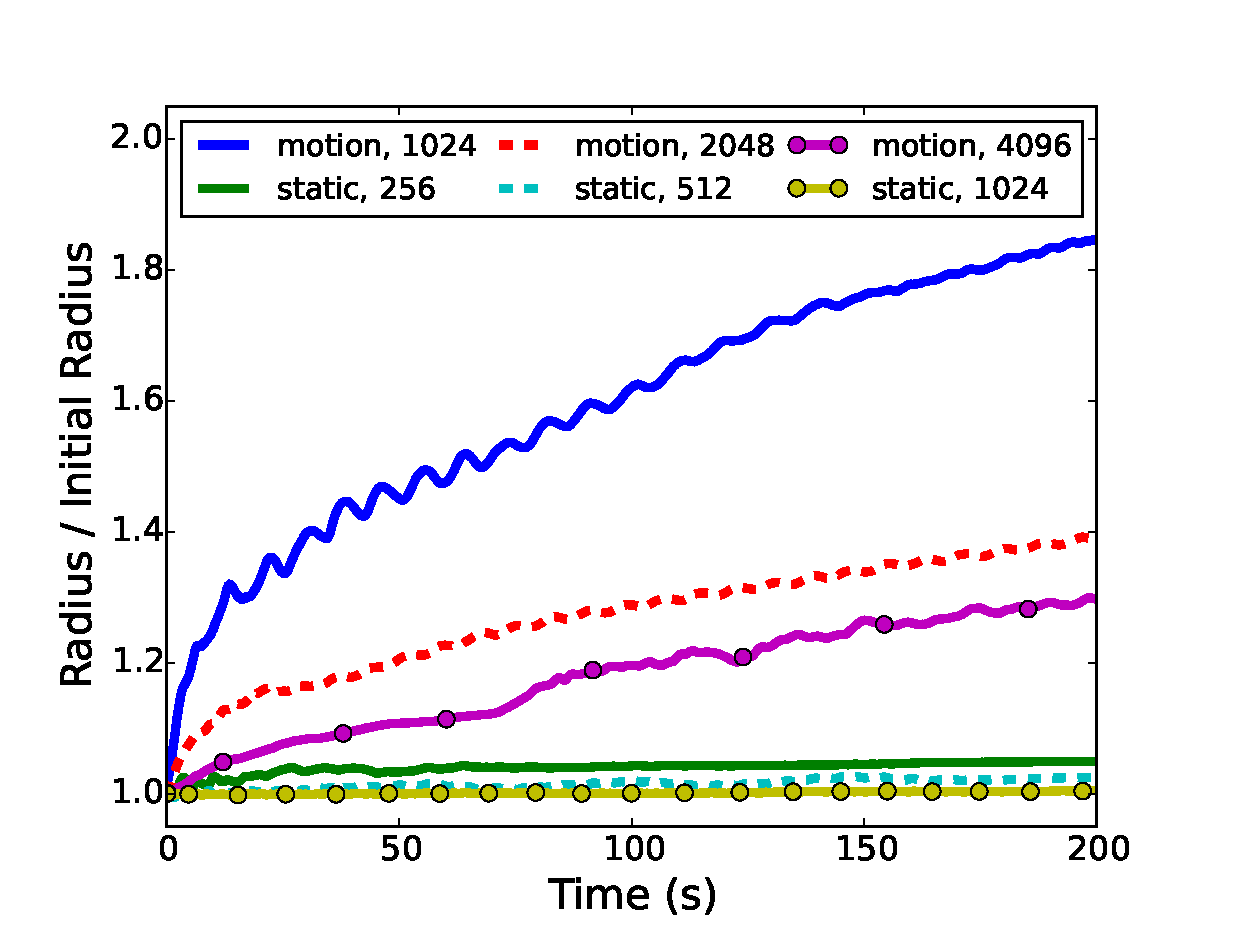
\includegraphics[scale=0.8,trim=0.1in 0.0in 0.6in 0.6in,clip]{plots/single_star_compare_1e3_radius}
  \caption[Moving star versus static star]
          {A variation on \autoref{fig:single_star_static_radius} where
           we now compare the ``static'' case to ``motion'' simulations where the 
           star moves across the grid at a fixed linear speed. The lines represent 
           the effective number of zones per dimension inside the stellar material;
           due to the expanded size of the grid in the ``motion'' case, the 
           physical resolution is the same in each column in the legend.
           \label{fig:single_star_compare_radius}}
\end{figure}

In \autoref{fig:single_star_compare_radius}, we take the results of
\autoref{sec:HSE} (the ``static'' case), and plot on top of it the
results of this new simulation (the ``motion'' case). We see
immediately that this bulk velocity causes the star to be much worse
at maintaining hydrostatic equilibrium. Not only is the absolute size
of the star significantly larger (nearly a factor of two at the lowest
feasible resolution we consider), but also there is a clear upward
trend in the size that has not terminated at any resolution by the end
of the simulation.  This again emphasizes the results mentioned
earlier, that we must be careful not to trust any simulation with
significant mass transfer if we are not confident that the mass
transfer is seeded in a controllable manner and free from numerical
noise.

\subsection{Keplerian Orbit}
\label{sec:kepler}

We now consider the phase of the binary system where the stars are orbiting each other 
at distances great enough that the initial orbits should be approximately Keplerian. 
There are a number of effects worth looking into here. For simplicity, we choose two 
cases to demonstrate the simulation behavior: an equal mass case of two $0.9\ \msolar$ 
white dwarfs, and an unequal mass case of $0.9\ \msolar$ and $0.75\ \msolar$ white dwarfs.
In both systems, the secondary should be stable against mass loss.
In each case, the initial orbital period is 100 seconds. For all simulations in this section,
we use the standard Euler equations that conserve linear momentum, and defer to \autoref{sec:mergers}
a description of the hybrid advection technique.

For some of the algorithms described earlier in this work, a single orbit of these 
systems is enough to examine their effects. In \autoref{sec:gravity_boundary_conditions},
we discussed the replacement of a monopole boundary condition solver for the gravitational 
potential with a more general multipole solver for the boundaries. To test the relevance 
of this effect, we considered a single orbit of the unequal mass system and measured 
the distance between the two white dwarf centers of mass at the beginning of the simulation and after 
the full orbital period. This distance should not change significantly over that timescale.
We performed this test for maximum multipole moments ranging from 0 (the monopole term) to 16.
The results are shown in \autoref{fig:gravity_bcs}. Terms in the boundary potential 
that vary faster than $r^{-5}$ are effectively negligible in determining the outcome of the orbit, 
justifying our typical choice of maintaining terms up to $r^{-7}$.

\begin{figure}[h!]
  \centering
  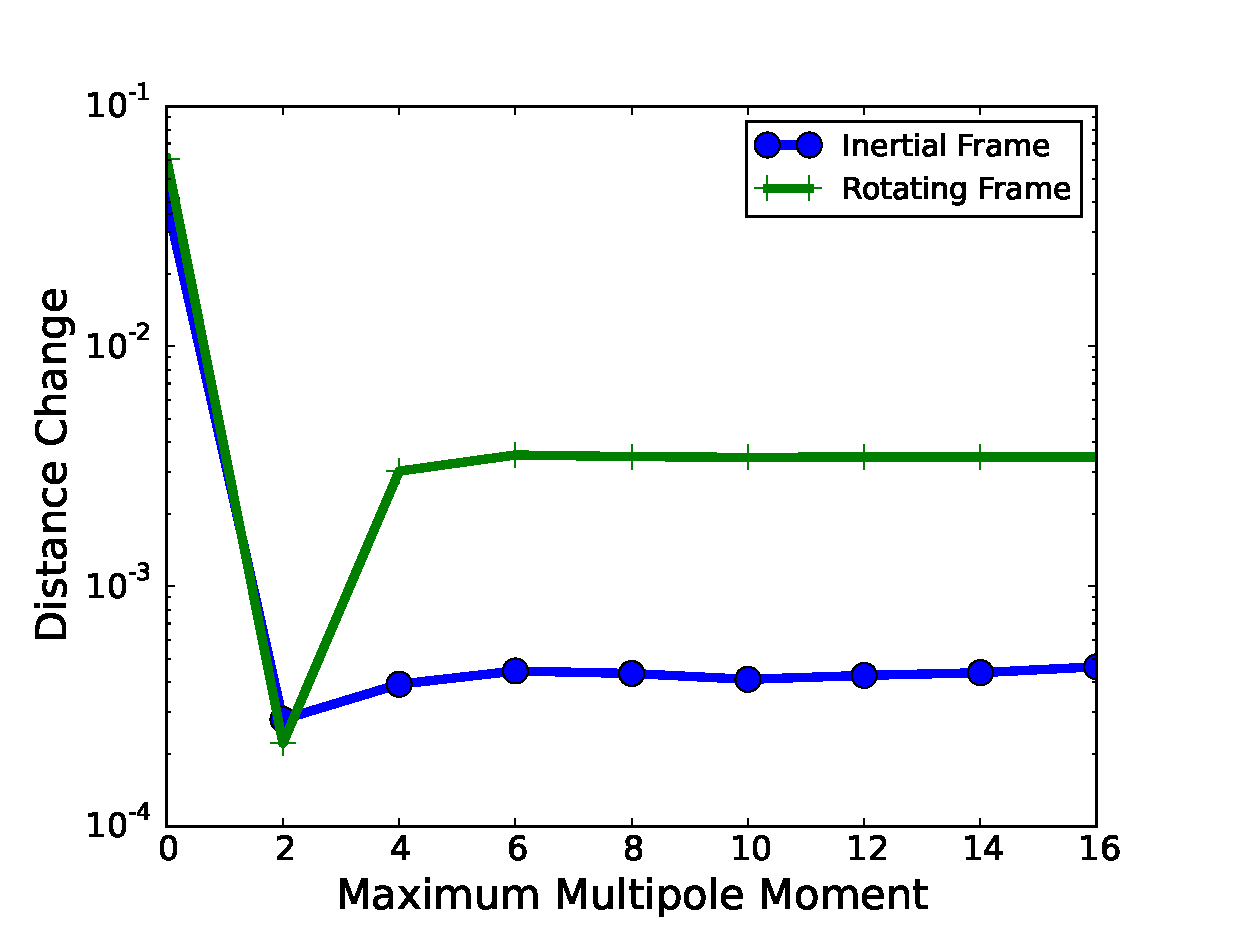
\includegraphics[scale=0.8,trim=0.1in 0.0in 0.65in 0.4in,clip]{plots/gravity_bcs}
  \caption[Distance change due to multipole boundary conditions]
          {Absolute magnitude of the relative change in the distance of two unequal mass white dwarfs after one orbital period. 
           The stars were evolved in an inertial reference frame. The horizontal axis is the number of terms or multipole moments 
           captured in the series expansion for the potential at the domain boundary.\label{fig:gravity_bcs}}
\end{figure}

Another diagnostic that we consider is the energy conservation of the
system. Recalling \autoref{sec:gravity_hydro_coupling}, there are
several different methods of applying the gravitational source term to
the hydrodynamics equations. In \castro\ we presently have four
options, controlled by the parameter {\tt castro.grav\_source\_type},
which we shorten to {\tt gs} for the present discussion. 
${\tt gs} = 1$ and ${\tt gs} = 2$ are variations on the standard 
cell-centered source term for gravity. The difference between them is that 
${\tt gs} = 2$ determines the value of the energy source term after the momentum
source term has been applied, while ${\tt gs} = 1$ uses the uncorrected
momenta in calculating $\rho \mathbf{u} g$. We have found ${\tt gs} = 2$ to be
more accurate. ${\tt gs} = 3$ is entirely different: after calculating
the new momenta, we reset the total energy to be equal to the internal
energy plus the kinetic energy. This approach has the virtue of ensuring that
there is no conflict due to discretization between the momentum and
energy equations, and also correctly ensuring that the gravitational
force does not directly change the internal energy---and thus the
temperature---of the fluid. However, it explicitly sacrifices total
energy conservation. ${\tt gs} = 4$ is the new conservative method of
evaluating the energy source terms at cell faces. The results for the
change in energy after a single orbit are seen in the first column of
\autoref{table:sources}. The first two versions give reasonable and
similar levels of energy conservation. The third has total energy
changes on the order of 100\%, but this itself does not have a severe
effect on the dynamics because in this scheme the total energy
variable is effectively a placeholder value of the kinetic energy plus
internal energy, rather than being evolved directly. The last scheme
is nearly two orders of magnitude better in energy conservation,
justifying the effort in varying the scheme.

In \autoref{table:sources} we show also the effects on energy conservation of using the inertial reference frame. 
We use ${\tt rs}$ for the \castro\ parameter {\tt castro.rot\_source\_type}.
Each option for ${\tt rs}$ is implemented in the same way as for
the gravitational source term, simply swapping out the gravitational acceleration
for the rotational acceleration (except for the improvement to the momentum update
for ${\tt rs} = 4$ described in \autoref{sec:rotation}). 
The ${\tt rs} = 0$ column means that rotation is turned off and we are 
in the inertial frame. We see that the choice of rotational coupling is much less important than the choice of gravity coupling. 
The ``conservative'' ${\tt rs} = 4$ is slightly better in energy conservation than the non-conservative, 
cell-centered ${\tt rs} = 2$ algorithm, but it is a small effect.

\input{plots/sources.table}

We are most interested in the stability of these systems over long
timescales. To this end, we consider the same systems as above, but
evolve them for 25 orbital periods. In 
\autoref{fig:circular_orbit_comparison} we illustrate the evolution of
these systems by plotting the center of mass locations of the white
dwarfs on the orbital ($xy$) plane. For the equal mass case in the
inertial reference frame, the curves fall nearly on top of each
other for most of the run, indicating that the stars are indeed 
orbiting at the initial distance, at least for a while. Towards the end 
of the run, however, the orbit starts to decay significantly, and the center-of-mass
distance of the two stars has decreased by about 10\% after 25 orbits.
We attribute this to non-conservation of angular momentum, which occurs 
because here we ran our code in the mode that  only explicitly conserves
linear momentum. This orbital decay resembles the effect seen by \citet{swc:2000}
for the case of neutron stars. In the unequal mass case, the magnitude of
the orbital decay is smaller but at the end of the run the secular decline
in distance is also visible. In both cases the stars would likely merge due
to numerical error after a long enough timescale.

The co-rotating frame is different.  For clarity of visualization, we
rotate these results back into the inertial frame before displaying
their orbits.  In both the equal and unequal mass cases, the centrifugal force 
pushes the stars outward toward a new equilibrium distance that is a few 
percent larger than its initial distance. At the end of the run, the system is 
relatively stable, with oscillations about the new equilibrium distance. In fact 
these oscillations occur too in the inertial frame, but they are much more pronounced 
here. In the unequal mass case this is coupled with severe precession of the orbit, 
which results in chatoic-looking orbits when viewed from the rotating reference frame. 
These result from the explicit numerical consideration of the Coriolis and centrifugal 
terms, which do not appear in the inertial frame. So while the rotating frame 
is clearly more stable against mass transfer than the inertial frame,
the cost is that the specific dynamics may be more suspect.

\begin{figure}[h!]
  \centering
  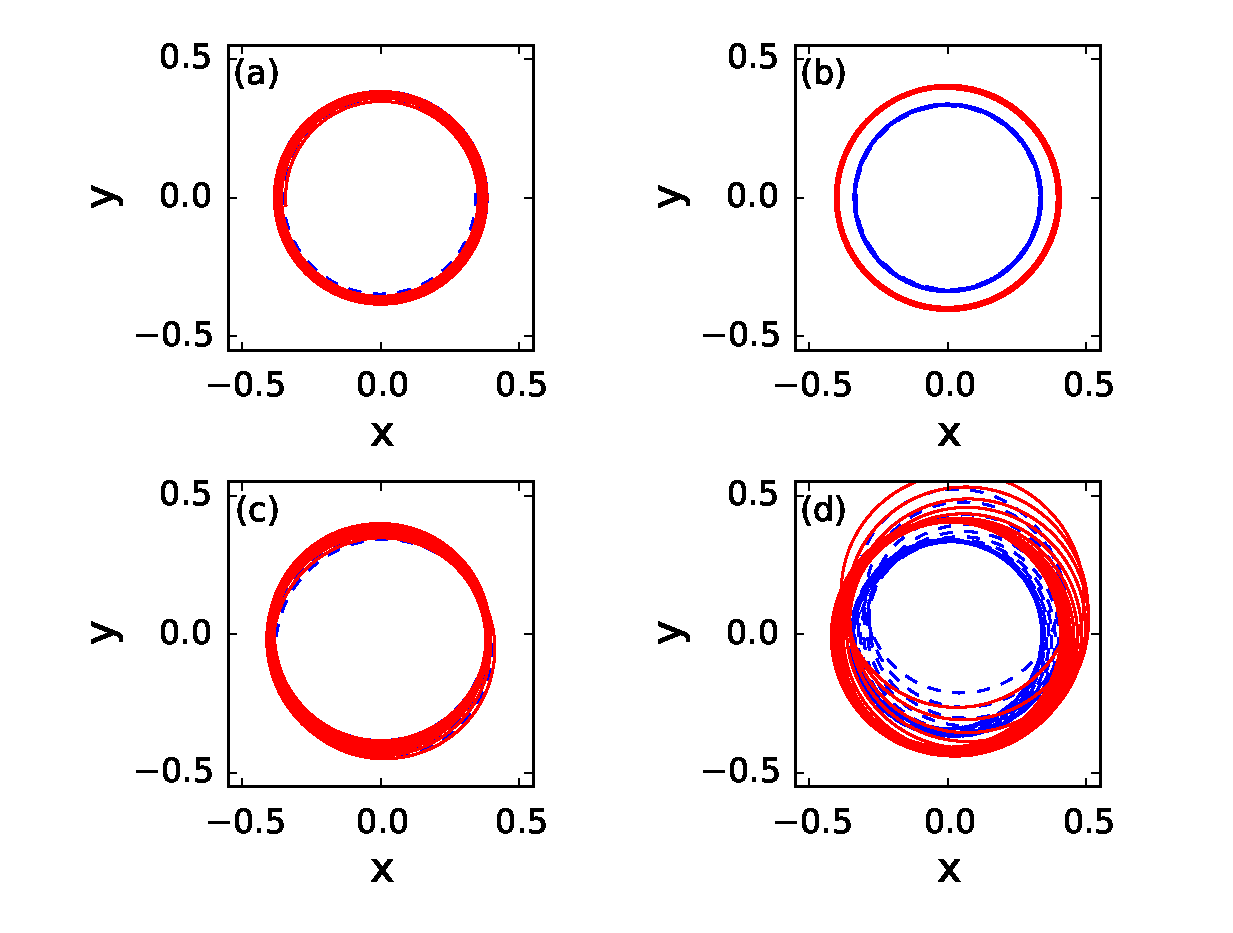
\includegraphics[scale=0.8,trim=0.1in 0.0in 0.1in 0.0in,clip]{plots/circular_orbit_comparison}
  \caption[White dwarf positions over 25 orbital periods]
          {Positions of the white dwarfs in the orbital plane for four
           cases evolved over 25 orbital periods.  The $x$ and $y$ axes are
           normalized to the size of the domain, so that $x = -0.5$ is the
           left edge and $x = 0.5$ is the right edge. The dashed blue curve
           is the position of the primary white dwarf, and the solid red
           curve is the position of the secondary. In plot (a) we have the
           equal mass system evolved in the inertial reference frame, and in
           plot (c) we have the same system evolved in a rotating frame,
           where the positions have been transformed back to the inertial
           frame for comparison.  Plots (b) and (d) are analogous but for the
           unequal mass system.\label{fig:circular_orbit_comparison}}
\end{figure}

Turning to the conservation properties of the system, we examine as
fairly typical cases the equal mass system in the inertial frame for
energy conservation (\autoref{fig:energy_conservation_equal}), and the
unequal mass system in the rotating frame for angular momentum
conservation (\autoref{fig:angular_momentum_conservation_unequal}).
For the former system angular momentum is conserved to within 10 percent over the 25
orbits, while energy conservation is about an order of magnitude
better. We note that while this is already a fairly good level of
energy conservation, it is not nearly as good as the results of
\citet{marcello:2012}. This is because we reset the internal energy to
a level corresponding to our temperature floor when it goes negative,
while \citeauthor{marcello:2012} do not reset and instead ignore the
internal energy if it is negative. The resets impose an artificial
floor on our ability to conserve energy, but they only happen in
low-density regions and do not much affect the large-scale dynamics.
Meanwhile, relative angular momentum conservation is not quite as good 
as relative energy conservation.  This is 
linked to the decline (or increase) in the size of the orbit. This
implies that we ought to be careful in concluding that at these
moderate resolutions we can safely evolve systems for many dozens of
orbits; this needs to be verified to ensure that an observed inspiral
and merger is physically (not numerically) motivated.

\begin{figure}[h!]
  \centering
  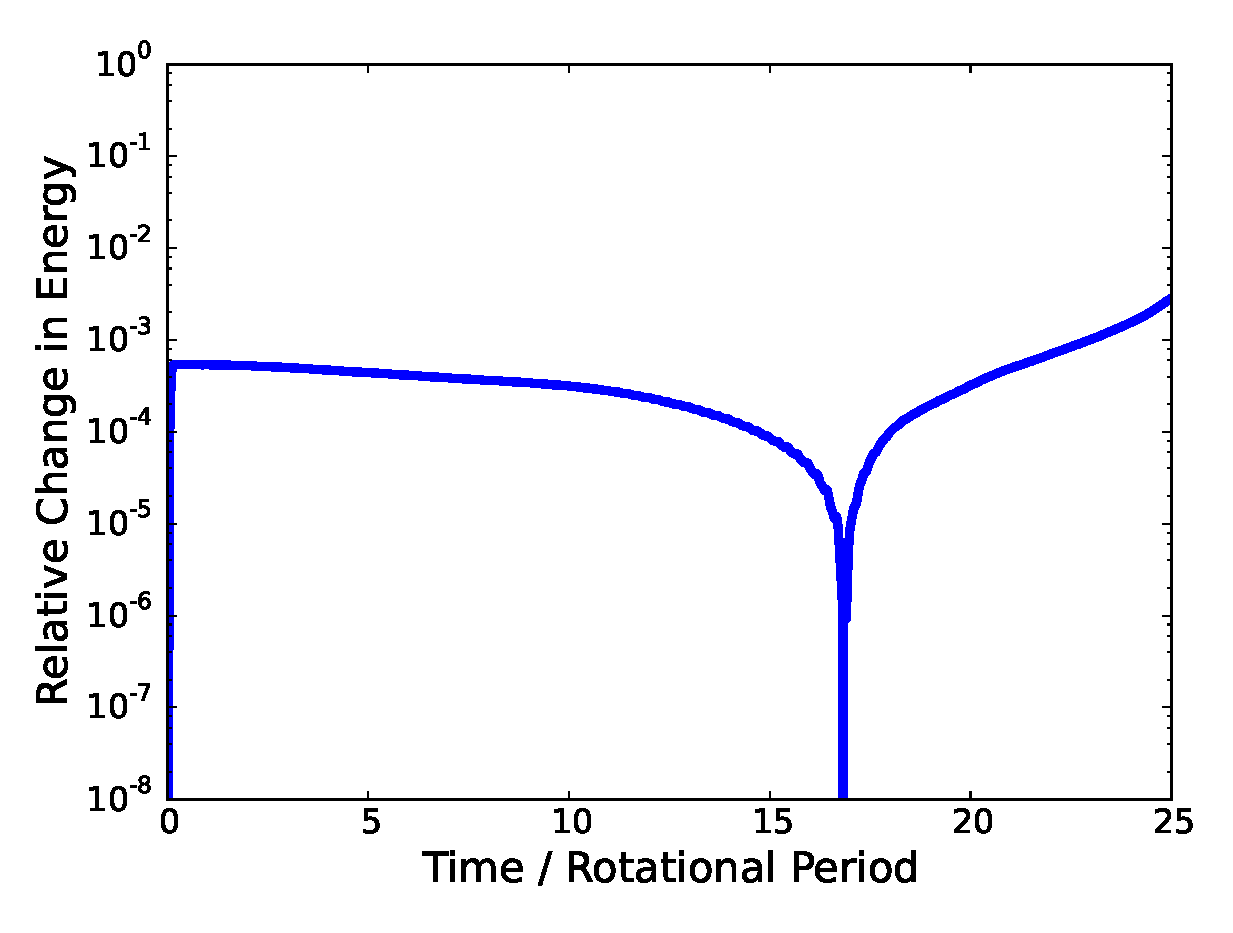
\includegraphics[scale=0.8,trim=0.1in 0.0in 0.1in 0.1in,clip]{plots/equal_energy_rot0}
  \caption[System energy over 25 orbital periods]
          {Absolute magnitude of the relative change in energy of two equal mass white dwarfs through 25 orbital periods,
           evolved in an inertial reference frame. The decline and recovery is a change in sign of the energy difference.
           \label{fig:energy_conservation_equal}}
\end{figure}

\begin{figure}[h!]
  \centering
  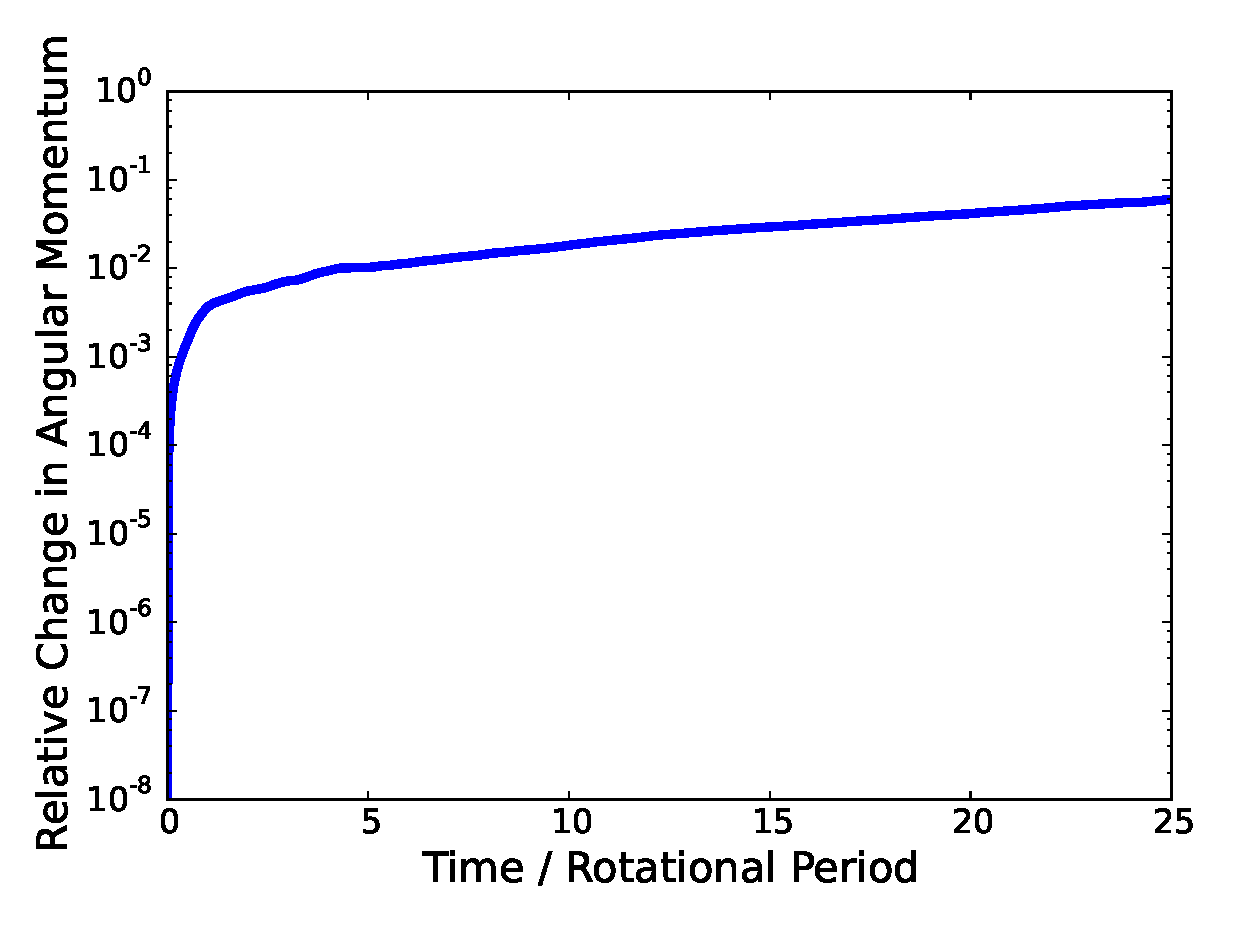
\includegraphics[scale=0.8,trim=0.1in 0.0in 0.1in 0.1in,clip]{plots/unequal_angular_momentum_rot1}
  \caption[System angular momentum over 25 orbital periods]
          {Absolute magnitude of the relative change in angular momentum of two unequal mass white dwarfs after 25 orbital periods, 
           evolved in a co-rotating reference frame. We consider only the component of the angular moment along the rotational 
           axis.
           \label{fig:angular_momentum_conservation_unequal}}
\end{figure}

As a simple verification test to ensure our gravitational wave calculations are correct, we plot the 
gravitational wave strain along the rotation axis for the first two periods of an unequal mass system. 
At this early time the orbit is circular and so to a good approximation we expect that the gravitational 
wave signal should be that of two point masses, whose positions are:
\begin{align}
  \mathbf{r}_P(t) &= -a_P\, \text{cos}(\omega t) \hat{x} - a_P\, \text{sin}(\omega t) \hat{y} \\
  \mathbf{r}_S(t) &= a_S\, \text{cos}(\omega t) \hat{x} + a_S\, \text{sin}(\omega t) \hat{y}.
\end{align}
Then the mass distribution is $\rho(\mathbf{r}) = M_P\, \delta^3(\mathbf{r} - \mathbf{r}_P) + M_S\, \delta^3(\mathbf{r} - \mathbf{r}_S)$.
From this it is straightforward to calculate the quadruopole tensor, take its second time derivative, and then apply the 
projection operator to get the gravitational wave polarizations along the rotation axis:
\begin{align}
  h_+ &= -4\frac{G\mu}{c^4 r}\left[G M_{\text{tot}} \omega \right]^{2/3}\, \text{cos}(2\omega t) \\
  h_\times &= -4\frac{G\mu}{c^4 r}\left[G M_{\text{tot}} \omega \right]^{2/3}\, \text{sin}(2\omega t).
\end{align}
$\mu$ is the reduced mass, while $M_{\text{tot}}$ is the total mass. From this we see that the 
gravitational wave frequency is twice the orbital frequency, and that the two polarizations 
are out of phase by $90^\circ$ in time. We compare this analytical expectation to the 
numerical results in \autoref{fig:gw_strain}. We find very good agreement in this case, and this 
level of agreement holds in the rotating frame as well.

\begin{figure}[h!]
  \centering
  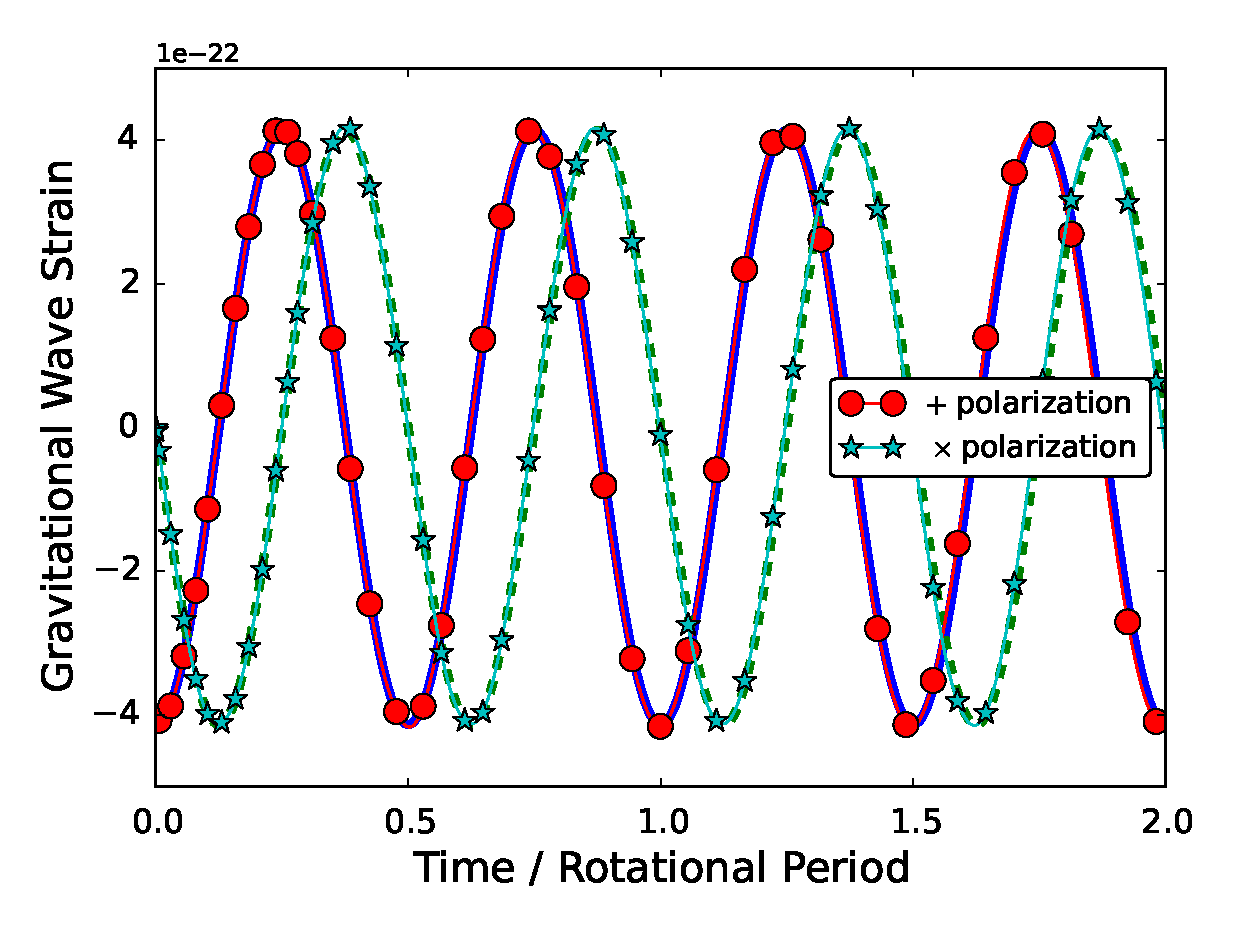
\includegraphics[scale=0.8,trim=0.1in 0.0in 0.1in 0.175in,clip]{plots/unequal_gw_rot0}
  \caption[Gravitational wave strain test]
          {Gravitational wave strain polarizations for the first two orbital periods of an 
           unequal mass system. The curves with markers are the numerical data, while the 
           curves without markers are the analytical results for two point masses.\label{fig:gw_strain}}
\end{figure}

Finally we consider whether the dynamical behavior of the system converges with resolution. 
In \autoref{fig:unequal_spatial_convergence_inertial} we plot the first full orbit for 
the unequal mass system, at three different resolutions in the inertial frame: our default 
resolution of $256^3$ zones, as well as a single level of refinement with a jump by a factor of 
two (effective resolution $512^3$) or a jump by a factor of four (effective resolution $1024^3$). 
It is clear that at the latter resolution (corresponding to physical resolution of 100 km), 
we have achieved convergent behavior. In the rotating frame, the results also show
convergent behavior but the convergence is not as fast with resolution as in the inertial frame; 
see \autoref{fig:unequal_spatial_convergence_rotating}. At the two higher resolutions the white dwarf
distance is qualitatively similar, and both are qualitatively different from the lower resolution. However,
quantitatively the two higher resolution runs are not as similar to each other as the analogous runs in the
inertial frame. Convergence with resolution is slightly slower in the rotating reference frame
because in the rotating reference frame a stable, unchanging circular orbit requires balance between
two forces with opposite sign (the gravitational and centrifugal forces), and slight perturbations from the
circular orbit are amplified by the effect of the Corolis force. In the inertial frame, these numerical instabilities
vanish, but the cost is that there is no centrifugal force to actively maintain the white dwarf distance,
which is why it is much more likely for the orbit to prematurely decay. In either case, these results suggest
at least a minimum resolution of 200 km for getting the dynamics qualitatively right. To put that into context,
consider that the parameter study of \citet{dan:2014} used 40,000 SPH particles per simulation, or (for an equal mass
binary) 20,000 particles per white dwarf. For, say, a $0.9\ \msolar + 0.9\ \msolar$ white dwarf binary on
a $256^3$ zone simulation grid, there are 20,000 zones that fit within a white dwarf. We do not
intend here to directly compare results between the two simulation methods. We limit ourselves to the
observation that at least for grid-based codes, a parameter study such as the ones performed by
\citet{dan:2012} and \citet{dan:2014} would likely not yield qualitatively convergent results if it were to use the
same effective mass resolution. Instead the number of zones inside each star should at least be doubled.

\begin{figure}[h!]
  \centering
  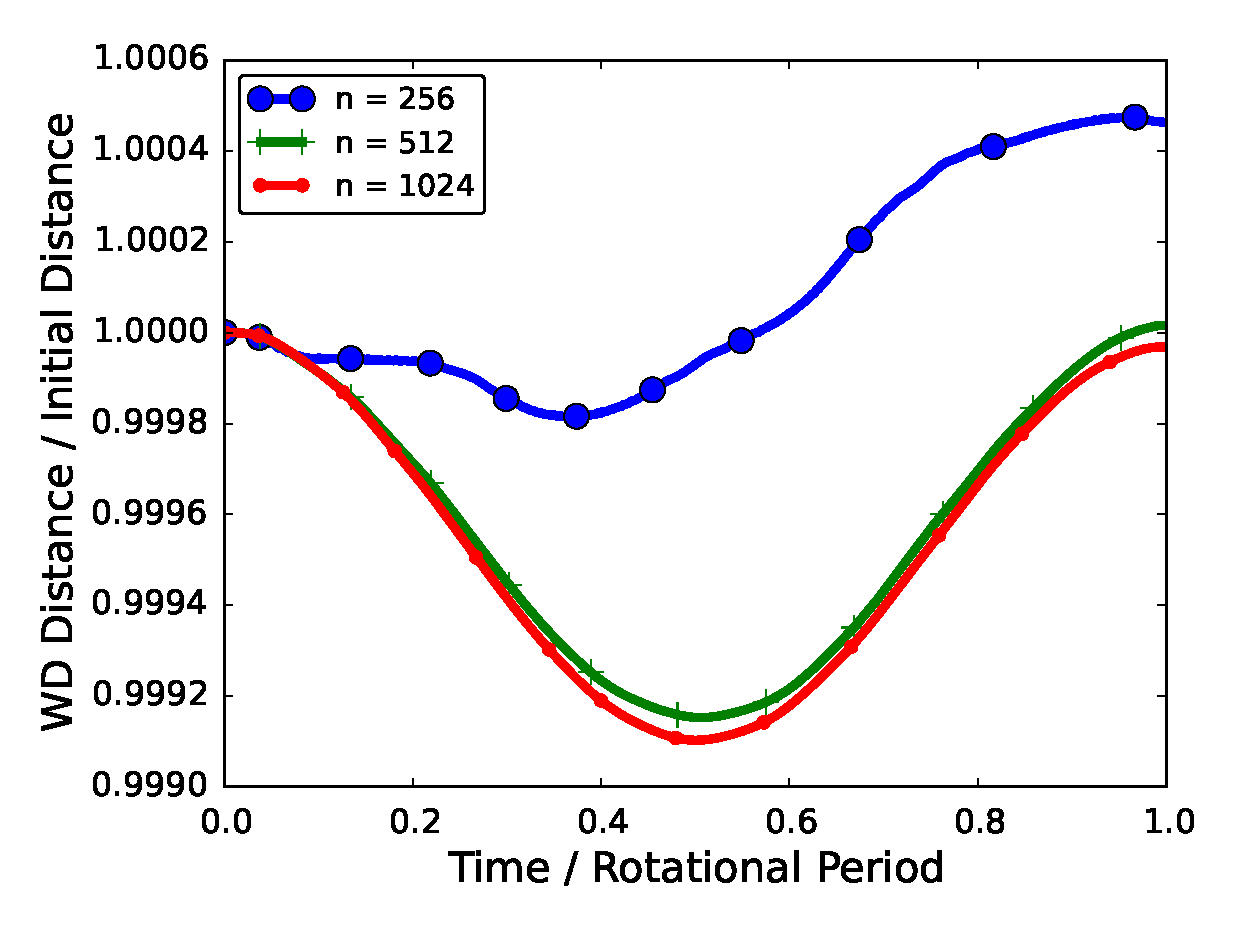
\includegraphics[scale=0.8,trim=0.1in 0.0in 0.1in 0.2in,clip]{plots/spatial_convergence_rot0}
  \caption[Distance between two unequal mass white dwarfs, inertial frame]
          {Distance between the two white dwarfs in the unequal mass system, for the first orbit.
           The distance is scaled by the initial orbital distance. 
           We plot at three different resolutions, corresponding to the number of 
           effective zones per dimension in the refined regions.
           \label{fig:unequal_spatial_convergence_inertial}}
\end{figure}

\begin{figure}[h!]
  \centering
  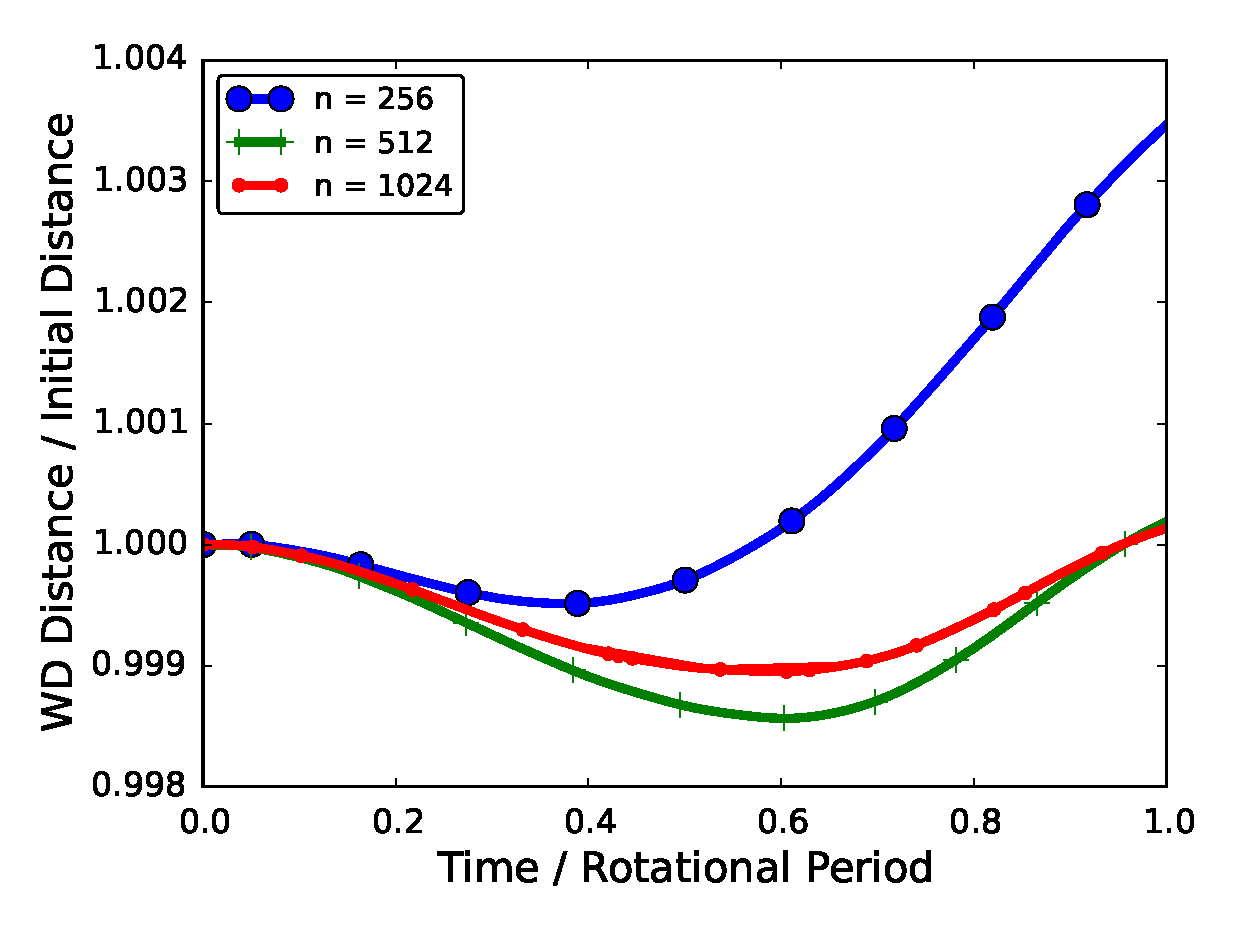
\includegraphics[scale=0.8,trim=0.1in 0.0in 0.1in 0.2in,clip]{plots/spatial_convergence_rot1}
  \caption[Distance between two unequal mass white dwarfs, rotating frame]
          {Distance between the two white dwarfs in the unequal mass system, for the first orbit.
           The distance is scaled by the initial orbital distance. 
           We plot at three different resolutions, corresponding to the number of 
           effective zones per dimension in the refined regions.
           \label{fig:unequal_spatial_convergence_rotating}}
\end{figure}



\clearpage
\section{Parallel Performance}
\label{sec:performance}

\castro\ is designed to be deployed on high-performance computing systems using 
many thousands of processors simultaneously. It is worth briefly examining 
our strategy for parallelizing the problem over many computational nodes 
and our performance in situations similar to production science simulations. 
This is especially true because some aspects of our approach to parallelism 
have changed since the first \castro\ paper \citep{castro}, and we have obtained improved 
performance in certain settings.

The \boxlib\ framework that \castro\ is based on domain decomposes each AMR level into a number 
of boxes that collectively span the level. These boxes are distributed to processors 
through MPI parallelism; each MPI task in general holds multiple boxes and 
an update includes a loop over all the boxes an MPI task owns. The distribution 
obeys a load-balancing algorithm that attempts to equalize the amount of work 
done by each processor. \boxlib\ contains a number of strategies for distributing 
work in this way, and by default uses a space-filling curve approach with a 
Morton ordering (e.g. \cite{sasidharan:2015,beichl:1998}). By experiment we have
found that the most efficient load-balancing strategy for our problem is often
actually a simple knapsack algorithm, though this depends on the size and layout of
the problem. In this approach, 
the amount of work owned by a processor is proportional to the number of grid cells 
associated with that processor, and the algorithm attempts to ensure that all 
processors have a similar number of total grid cells. We demand an efficiency of 0.9,
meaning that the average workload per processor should be no smaller than 90\% of the 
maximum workload found on any processor. We find that in practice the 
performance is largely insensitive to this choice.

The size and shape of grid boxes is an important consideration for efficiency. 
Boxes that are very small suffer from a host of problems, including the larger 
amount of communication required between hydrodynamics solves. Additionally, 
the multigrid solver is less efficient if the boxes are small because there 
are fewer available levels for coarsening and performing V-cycles. Furthermore,
the ratio of the number of ghost zones to physical zones becomes larger for small
boxes, and is above unity for a $16^3$ box. Conversely, boxes that are too large
often mean that there isn't enough work to go around when we 
have a large number of processors. Good performance is the result of a careful 
balance between these two effects. For mergers, on the lower end, we require that
all boxes be a multiple of 16 zones in each dimension; multigrid efficiency sharply
decreases if this factor is any lower. On the upper end, we select the maximum grid size 
based on the number of processors we use and the total number of cells in the 
simulation. This size will therefore in general vary on different AMR levels. 
Generally we select a value in between 32 and 64 zones per dimension. For collisions,
when nuclear burning usually dominates all other effects including the communication cost,
we allow the minimum box size to become smaller (sometimes as small as 8 zones per
spatial dimension); we do not need to burn on the ghost zones, as we can replace it with
a communication step that fills the ghost zones using data from other boxes.

We use OpenMP to accelerate the work associated with the boxes owned
by each MPI task. Originally \castro\ used OpenMP to accelerate
individual loops in the hydrodynamics routines, such as the
piecewise-parabolic edge state reconstruction and the conservative
flux update. However, there is a significant amount of overhead
associated with generating a new OpenMP region at each of the many
different loops in a hydrodynamics algorithm. This makes such a
strategy sub-optimal for use on many-core processors and GPUs. \castro\ has
recently switched to a tiling approach where an OpenMP region is
generated at the start of the hydrodynamics routine and the individual
threads separately work on different partitions of each box \citep{boxlib-tiling}. This
results in much less overhead for the threading. In general we obtain
more efficient simulations than could be obtained using MPI only,
because there are fewer boxes and thus less communication for a given
number of processor cores. We have also made significant progress in
developing an approach to evaluating the hydrodynamics and microphysics modules on GPUs,
which will allow us to take advantage of the significant computational resources embedded in
GPUs on certain systems.

\begin{figure}
  \centering
  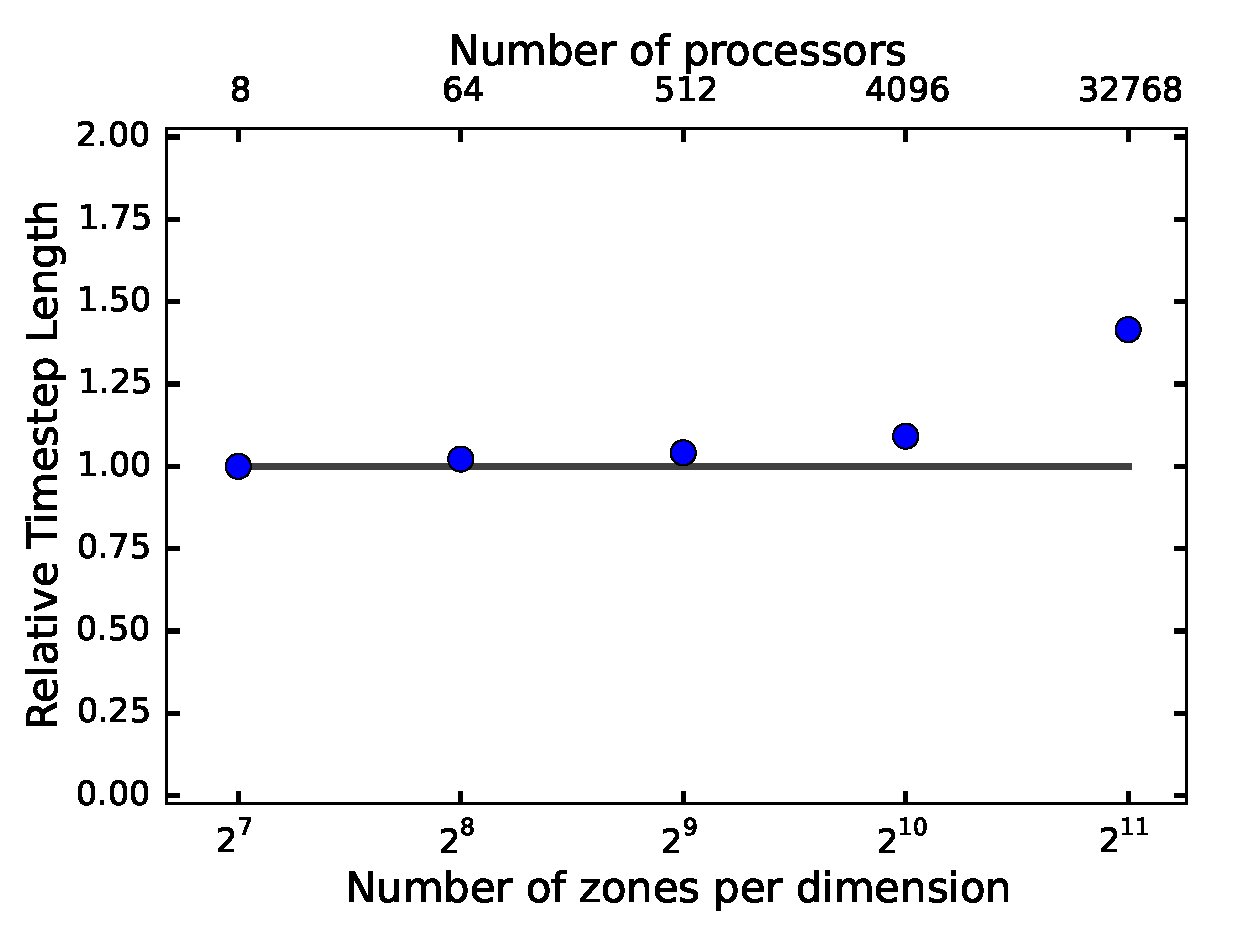
\includegraphics[scale=0.8]{plots/weak_scaling}
  \caption[\castro\ weak scaling test]
          {\castro\ weak scaling test, performed on Blue Waters at 
           NCSA. Each processor had a fixed amount of work, and we increased the 
           number of simulation zones in concert with the number of processors. The 
           solid curve represents perfect weak scaling, while the blue circles show 
           \castro's performance at each processor count. The vertical axis measures 
           the median time per timestep, normalized to this value for the smallest 
           processor count.
           \label{fig:weak_scaling}}
\end{figure}

To examine the parallel performance of \castro, we performed both
strong scaling and weak scaling tests on the Blue Waters machine at
the National Center for Supercomputing Applications. For the weak
scaling test, whose results are shown in \autoref{fig:weak_scaling},
we ran a uniform grid binary white dwarf simulation for resolutions of
$128^3$ zones through $2048^3$ zones. The number of processors was
scaled with the number of zones so that each processor had the same
amount of work; the smallest test used 8 processors and the largest
used 32,768 (note that the number of processor cores on a Blue Waters
node is twice the number of floating point units on that node). The
test was run for 10 timesteps, with each timestep including two
Poisson solves and a hydrodynamics update (though for a uniform grid
calculation we generally do not need to perform any multigrid
iterations for the first Poisson solve in a timestep, since the
density distribution has not changed since the end of the last
timestep). We disabled plotfile and checkpoint writing, as well as
calculation of diagnostic information (the latter can contribute to a
significant fraction of the run time at large processor counts if
computed every timestep). We computed the median wall time required
per time step for each simulation, and then normalized this to the
median time per timestep for the smallest simulation. We find
excellent weak scaling through 4,096 processors. At the largest run,
the simulation time required is slightly less than 1.5 times the amount
required for the smallest simulation.  This is due entirely to the
increased cost of the multigrid Poisson solve in each timestep and
this cannot be mitigated except by improving communication or
computation efficiency in the multigrid solver. We observe that this
weak scaling behavior with Poisson gravity is a significant
improvement over the results presented in the first \castro\ paper.

\begin{figure}
  \centering
  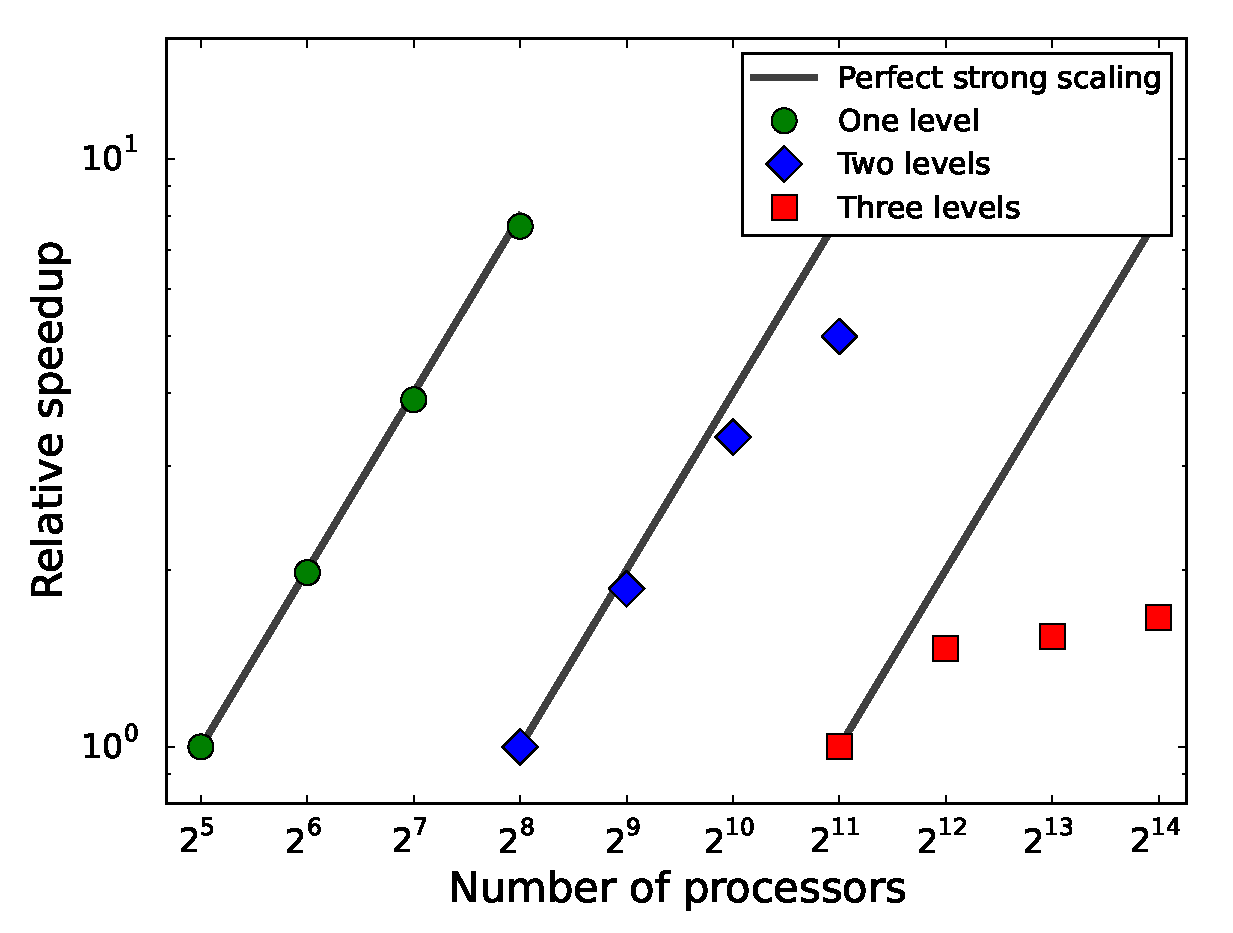
\includegraphics[scale=0.8]{plots/strong_scaling}
  \caption[\castro\ strong scaling test]
          {\castro\ strong scaling test performed on the Blue Waters machine at
           NCSA. The vertical axis measures the median time per timestep, and the 
           horizontal axis measures the number of processors in the simulation. Data 
           points are normalized to the time per timestep for the smallest number 
           of processors. The green circles show the data for a simulation with one 
           AMR level (a single uniform grid), the blue diamonds show the data for a simulation with two AMR
           levels (one coarse and one fine), while the red circles show the data 
           for a test with three AMR levels (one coarse and two fine). The fine levels 
           increase the resolution only in the regions around the stars. For each case 
           we draw a solid curve representing perfect strong scaling.
           \label{fig:strong_scaling}}
\end{figure}

The strong scaling test we performed uses a grid setup similar to what we 
use for well-resolved binary simulations. With only a uniform coarse grid, 
there are approximately $2 \times 10^7$ zones. With a single refined level, 
we have approximately $2 \times 10^8$ zones, typically spread over $\sim 2000$ grids.
On a second refined level, there are a similar number of zones and grids 
(the volume covered by this level is smaller, which offsets the greater resolution).
We ran a scaling test for all three cases, with the 
highest processor count in each case chosen so that the number of 
MPI tasks is similar to the number of grids. There are no gains 
to be achieved from further parallelism. The results are found in 
\autoref{fig:strong_scaling}. We find excellent scaling for low to moderate numbers 
of processors. Parallel efficiency is well maintained when there are 
at least 2 grids per processor. The 
scaling behavior worsens at the highest processor counts, but this is 
an expected consequence of processors becoming work-starved. At the highest 
processor count in this test, there is approximately only one grid per processor. In general 
we find very good strong scaling behavior in the regime we are presently 
interested in, simulating the early phases of a simulation at moderate 
resolution. The strong scaling behavior is acceptable, though not perfect, 
at very large processor counts when self-gravity is considered.



\clearpage
\section{White Dwarf Collisions}
\label{sec:collisions}

\subsection{Parameter Study}
\label{sec:collision_parameters}

Before turning to the effect that adaptive mesh refinement has on WD collisions,
we will first examine the effect of a number of other code parameters. For most
of the following we will use two-dimensional axisymmetric simulations which have
impact parameter $b = 0$, unless otherwise specified, and we will stick to a
moderate resolution (we use only the coarse grid described in \autoref{sec:software}).
For all simulations in this section, we use a pair of $0.64\ \msolar$ WDs, a binary
system that has been studied in most of the collision papers to date. This allows
us to cheaply test how the collision responds to many effects. One limitation of
this is that we will not find out exactly how a simulation differs in the case of a
high-resolution 3D run when these parameters changed. Another is that we will not
perform a full parameter study where we consider the full non-linear dependence of
all parameters on all other parameters; here we are merely interested in qualitative
trends that will help to understand the limitations of WD collision simulations.

With those caveats in mind, let us consider the tests and the results we obtained.
Our primary metric for the following tests will be the amount of $^{56}$Ni generated
in the collision, as this is the parameter most directly related to the observable
quantities of interest for Type Ia supernovae. Specifically, we collect information
at the end of every timestep about the total amount of nickel on the grid (in solar
masses), and we will use the maximum value of this nickel mass. When the stopping
criterion described in \autoref{sec:software} is used, this nickel mass is generally
constant or decreasing by the end of the run. The typical amount of nickel mass generated
for our runs at low resolution is $0.2\ \msolar$, which is significantly lower than
that obtained by \cite{raskin:2010} and \cite{kushnir:2013} for the same problem.
We will discuss this in \autoref{sec:collision_resolution}.



\subsubsection{Timestepping}
\label{sec:collision_parameters:timestepping}

For the standard self-heating burns that we use, the most important parameters we
examined come from the timestep limiting scheme described in \autoref{sec:burnerhydrocoupling}.
The parameters $f_{be}$ (from \autoref{eq:timestep_e}) and $f_{bX}$ (from
\autoref{eq:timestep_X}) control the size of the timestep as a function of the
burning rate. As the timestep gets smaller, the error due to the Strang splitting
scheme coupling the reactions and the burning also gets smaller, and we expect
that the results become more accurate.
\begin{figure}[ht]
  \centering
  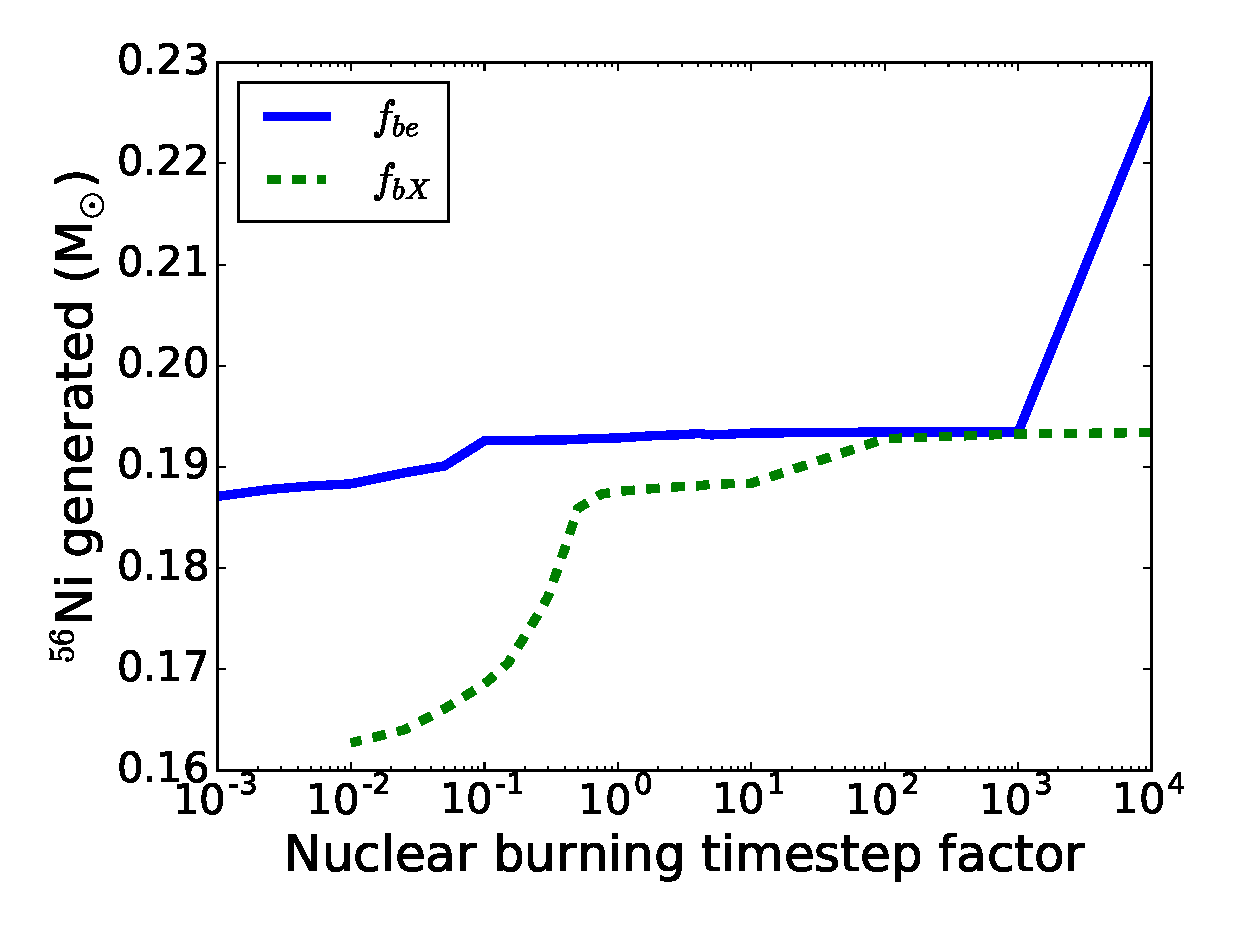
\includegraphics[scale=0.8]{{{plots/dtnuc_max_Ni56_m_P_0.64_m_S_0.64}}}
  \caption[Nickel production dependence on the burning timestep factor]
          {Nickel production as a function of the timestep factors $f_{be}$
           (solid blue, limiting the timestep on changes in internal energy) and
           $f_{bX}$ (dashed green, limiting the timestep on changes in species).
           For a given $f_{be}$, $f_{bX}$ with the same value typically limits
           the timestep by at least an order of magnitude more.
           \label{fig:timestep_factor}}
\end{figure}
\autoref{fig:timestep_factor} demonstrates the effect of both parameters on the nickel
production. As either $f$ becomes small, the restriction on the timestep becomes quite
severe: for $f_{bX} = 0.01$, the minimum timestep in the simulation is smaller than
$2 \times 10^{-9}\ \text{s}$ and the full simulation requires over 750,000 timesteps.
Yet it is clear that even for this steep value of the limiter, which is much stricter
than the limiter used in, e.g., \cite{hawley:2012} and \cite{raskin:2010}, the
simulation has not fully converged in nickel production. These limiters are somewhat
redundant in the sense that a given $f_{bX}$ corresponds to another (higher) $f_{be}$,
as is evident by the fact that on the graph the curves look similar in shape but with
a horizontal offset.

We also examined the effect of the method used to enforce the limiting, using the
four limiting modes discussed in \autoref{sec:burnerhydrocoupling}. The results are shown
in \autoref{table:burninglimitermode} for the case $f_{be} = 0.3$ (we did not use
limiting with $f_{bX}$ for this test). The two modes that use the full last timestep's
worth of information to estimate $\dot{e}$ yield a slightly larger nickel mass than the
two modes that only use more recent information, but the difference is negligible.

\input{plots/burning_limiter_mode_m_P_0.64_m_S_0.64.tbl.nodeluxe}

For all remaining tests in this section, unless otherwise stated, we take $f_{be} = 10^2$
and disable limiting with $f_{bX}$ by setting it to a large number. This choice is a balance
between accuracy and efficiency: we avoid the obviously wrong answers that occur for $f_{be} > 10^3$
while ensuring that the timesteps are long enough that the following tests are computationally
inexpensive.

\subsubsection{Nuclear Network}
\label{sec:collision_parameters:network}

Now we move to a discussion of the effect of including various isotopes
in the nuclear reaction network. In particular we compare the \isoseven, \aproxthirteen,
\aproxnineteen, and \aproxtwentyone\ reaction networks. In all cases we run
the same problem setup, and the unused isotopes (everything but carbon and oxygen)
have their mass fractions in every zone set to a negligibly small number at initialization.
\autoref{table:networks} lists the $^{56}$Ni generation and total energy generation (determined
by subtracting the initial energy from the final energy). The energy generated in the latter
three cases agrees remarkably well, with a less than $0.5\%$ difference. \aproxthirteen\
over-generates nickel at the $2\%$ level compared to the networks with more isotopes, a reasonably
small difference. On the other hand, agreement with \isoseven\ is not very strong, as \isoseven\
generates far too much nickel and far too little energy. Nevertheless while the quantitative
agreement is not there, the collision looks qualitatively similar compared to the evolution with
more complicated networks, so while \isoseven\ should not be used for predicting nucleosynthetic
yields in production science runs, it may still be fair for use in proof-of-concept studies.

\input{plots/networks_m_P_0.64_m_S_0.64.tbl.nodeluxe}

\isoseven\ also has the peculiar property that after the detonation had passed through the WDs,
the region at the central contact point did not fully stop burning, yielding a quasistatic energy
release that added a couple of million extra timesteps to the simulation (in addition to the few
hundred it normally takes) before we manually terminated the run. The full effect of these additional
timesteps only amounted to a $10^{-4}$ relative change in the nickel production. By examining the behavior
of zones near the collision point, we discovered the reason for this. The zones in question have a composition that
is approximately $98\%$ Ni and $2\%$ He by mass. For this combination, a direct evaluation of the RHS in
comparison to, say, \aproxthirteen, reveals that $dX/dt$ for these isotopes is off by many orders of magnitude.
This is a consequence of the choice inherent to the network to assume that the isotopes in between $^{28}$Si
and $^{56}$Ni are in an effective equilibrium state. So an advective update that yields even a small change
to the abundances in the zone will very strongly knock the zone out of equilibrium with respect to the burn
step following the advective update. This then causes the burning timestep limiter to kick in and make the
timestep very small so that the advective changes do not cause such strong effects on the burning equilibrium.
This effect is an argument against the use of \isoseven\ for explosive, non-hydrostatic burning problems.

\subsubsection{Burning Mode}
\label{sec:collision_parameters:burningmode}

In \autoref{sec:burning} we observed that there are several alternatives to the traditional
self-heating approach in a burn. These alternatives are relevant to a collision problem because,
as pointed out by \cite{raskin:2010} and \cite{kushnir:2013}, it is possible for a typical
zone in our simulation to release a very large amount of energy in a burn before it is cooled
off by a subsequent hydrodynamic expansion step, leading to the numerically unstable burning
problem described in \autoref{sec:unstable_burning}. \autoref{table:burningmode} lists nickel
production for the four burning modes described earlier. The hydrostatic burn does produces
slightly more nickel than the self-heating burn, consistent with the idea that by limiting the
energy release from early carbon burning, we can forestall a detonation which is numerically
spurious. Yet the difference is only about 5\%. The reason is that the hydrostatic burn controls
the energy release during the burn, but \textit{not} what happens in the rest of the hydrodynamics
step. And in the hydrodynamics step, the \castro\ algorithm performs multiple EOS calls to ensure
that the temperature is synchronized with the internal energy at various points in the update.
So in practice there is a temperature change due to the burn for our problem. This seems inevitable
for any hydro code unless the hydrodynamics update includes an explicit equation for $T$ that is
independent of what is happening for the internal energy. Similarly, the hybrid burn does not
affect the total nickel production relative to the hydrostatic burn. The hybrid burn only changes
the behavior for zones that have a net negative energy release from the hydrostatic burn, which
occurs only after we have burned to NSE.

\input{plots/burning_mode_m_P_0.64_m_S_0.64.tbl.nodeluxe}

In contrast, the suppressed burning mode (modeled after \citet{kushnir:2013}) produces only about
$5 \times 10^{-4}\ \msolar$ of $^{56}$Ni. In a suppressed burn, we ensure that at every evaluation
of the right-hand-side vector for the nuclear network integration, all quantities are scaled by the
same factor, with this factor ensuring that the energy release is not large enough to permit a
spurious detonation. This seems to be equivalent to the method used in \citet{kushnir:2013}. We
reproduce their claim that this suppresses the detonation until later in the collision, after more
material has approached the stalled shock. We also observe that, for a given resolution, the simultaneous
detonations occur slightly outside the initial contact point, near the edges of the stalled shock. They
establish as the main source of error in simulations that produce too little nickel. However, we find
that the resulting detonations are not strong enough to convert a significant amount of material to NSE
conditions; instead, only QSE conditions are reached near the center of the collision, leaving a significant
amount of silicon and sulfur on the domain that is not further processed. This may be a consequence of
the low resolution we are using here; see the discussion on the properties of the detonation in
\autoref{sec:collision_resolution}.



\subsubsection{Impact Parameter}
\label{sec:collision_parameters:impactparameter}

As the impact parameter varies for a head-on collision, the cross-section of the contact
zone between the two stars varies in size and geometry. In \autoref{fig:impact_parameter}, we
see the dependence of the nickel production on the impact parameter $b$, measured in units
of the WD radius. This test was performed using the 3D setup at our usual base resolution of
400 km. For computational efficiency, timestep limiting based on burning was disabled.
We sampled at $b = 0.0$, $0.01$, $0.02$, $0.03$, $0.04$, $0.05$, and then increasing
in increments of $0.05$. Relative to $b = 0$, there is a slight increase in nickel production for small
but non-zero $b$, which then declines with increasing $b$ except for a bump at $b = 0.5$.
For $b \ge 0.7$, no detonation forms at all, and the merged object remains a stable C/O WD
with $M = 1.2\ \msolar$ at least until $t = 100$.

It is worth nothing that for $b = 0.0$ the nickel production is a bit smaller for the 3D simulation
than its equivalent 2D simulation, the default case described above. There are differences both in
the size of the timestep (which as we saw in \autoref{sec:collision_parameters:timestepping} plays a role in
the total nickel production) and in the discretized nature of the stars; the assumption of perfect
azimuthal symmetry inherent to the 2D simulation breaks down for the 3D simulation, especially at
low resolution, since the zones are rectangular.

\begin{figure}
  \centering
  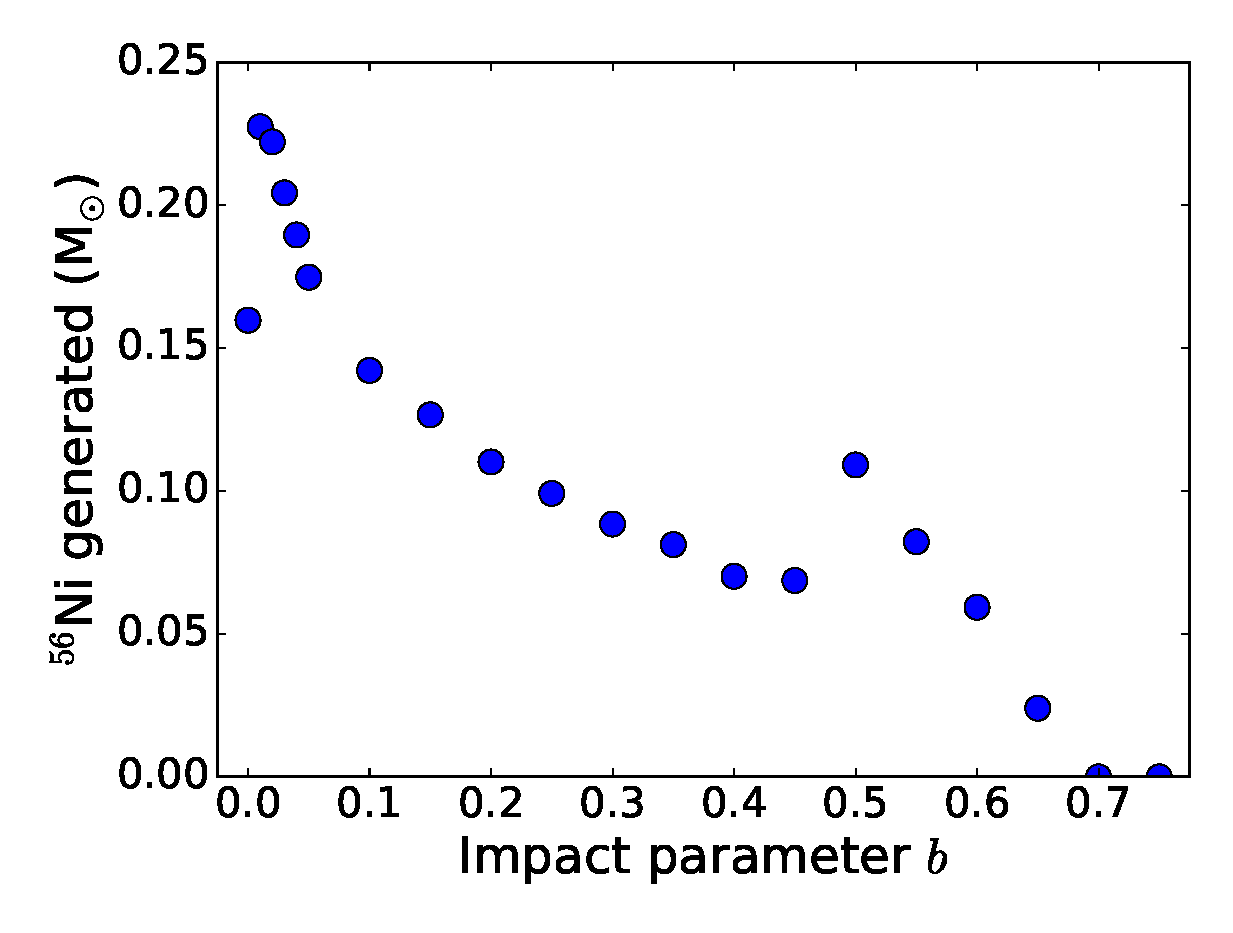
\includegraphics[scale=0.8]{plots/impact_parameter}
  \caption[Nickel production dependence on the impact parameter]
          {$^{56}$Ni generation as a function of the initial WD impact parameter for
           a $0.64\ \msolar$ + $0.64\ \msolar$ WD collision.
           \label{fig:impact_parameter}}
\end{figure}



\subsubsection{Other Parameters}
\label{sec:collision_parameters:other}

We tested a few other parameters that ended up having no serious effect on the outcome.
The dual energy parameter $\eta_2$ described in \autoref{sec:hydrodynamics} can have a
minor effect on the nickel production, yielding variations on the order of a few percent,
but there is no clear pattern. The dual energy parameter $\eta_3$ has no effect on the
outcome: the answer is the same for $\eta_3 = 0$ and $\eta_3 = 1$, which makes sense
because all of the reacting regions have a low enough kinetic energy relative to their
total energy such that the internal energy variable is always kept in sync with $(E - K)$.
(We did not look at $\eta_1$ because that has a direct effect only on the hydrodynamics,
not the reactions.) We also tested whether our choice for the temperature floor mattered
by lowering it to $10^6\ \text{K}$ and $10^5\ \text{K}$, and this had no effect on nickel
production. It does allow parts of the WDs to become colder as they move (see
\autoref{fig:initial_collision_state}), due to numerical
errors in the advecting flow (the Helmholtz equation of state is very insensitive to
temperature, so even small changes in the internal energy can create very large changes
in the implied temperature), but the amount of energy injected by the collision is so
large that the final result is insensitive to whatever the initial temperature of the
WDs were. We also checked whether there was any consequence of our choice to disable the
burning for small enough $\rho$ and $T$. Lowering the minimum $\rho$ for reactions to
$10^0\ \text{g cm}^{-3}$ from $10^6\ \text{g cm}^{-3}$ had a negligible effect,
and varying the minimum $T$ for reactions from $2 \times 10^{7}\ \text{K}$ to
$4 \times 10^{8}\ \text{K}$ also had no meaningful effect.

The choice of the WD composition to be equal carbon and oxygen by mass is a common
choice in the literature and is broadly comparable to what stellar evolution codes
yield for WDs of this mass. Still, it is an arbitrary approximation, especially the
insistence that the composition is uniform throughout the WD. In \autoref{table:co}
we list the nickel production as a function of the initial carbon mass fraction.
This can have a few percent impact on the outcome for the plausible values we tested.
In future work we may look at the effect of a more realistic progenitor structure,
including the effects of a helium shell on the surface of the WDs \citep{holcomb:2015}
and a non-uniform interior structure.

\input{plots/co_frac_m_P_0.64_m_S_0.64.tbl.nodeluxe}



\subsection{Resolution Dependence}
\label{sec:collision_resolution}

To test the effect of adaptive mesh refinement based on the burning rate, specifically
based on the criterion in \autoref{eq:burning_limiter_2} with the safety factor set to
$f_s = 0.1$, we performed a series of 2D calculations starting with the coarse grid and
allowing refinement up to a predetermined maximum jump in refinement. Each successive
run allowed a factor of two jump in refinement relative to the last. For this set we did
not enable timestep limiting other than the usual hydrodynamic limiting. We plot the nickel
production from this series of runs in \autoref{fig:dxnuc_nickel}. The additional resolution yields
a nearly monotonic increase in the nickel production, which is modulated both by the smaller
timestep on the finer levels and by the detonation being effectively slowed down by the
ability of the zones to more quickly disperse over-pressure generated by the nuclear burning.

\begin{figure}[h]
  \centering
  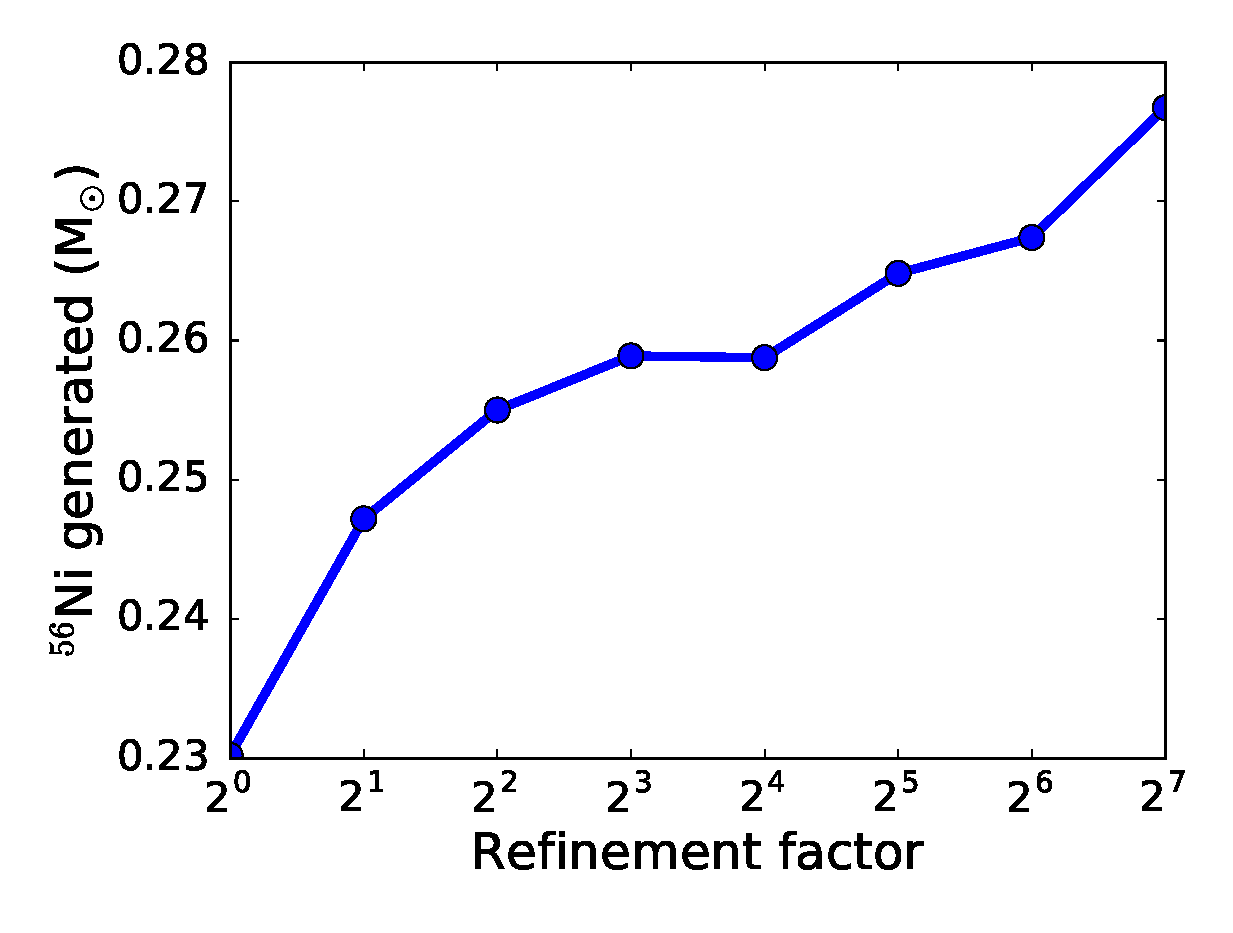
\includegraphics[scale=0.8]{{{plots/dxnuc_m_P_0.64_m_S_0.64}}}
  \caption[Nickel production as a function of refinement based on burning rate]
          {$^{56}$Ni production as a function of the maximum refinement factor
           relative to the coarse grid. Refinement is only applied after
           \autoref{eq:burning_limiter_2} is violated, and typically maximal
           refinement is achieved for the duration of the explosive burning.
           \label{fig:dxnuc_nickel}
          }
\end{figure}

Taking a cue from \cite{kushnir:2013}, we also examined the nature of the detonation itself.
For the default collision case we use, the detonation occurs at approximately $t = 7.5$ seconds
(this is offset by about 5 seconds compared to \citeauthor{kushnir:2013} because they started
the WDs at a smaller initial distance). \autoref{fig:dxnuc_detonation} is a plot of the inner
10\% of the domain 0.05 seconds after the detonation initiated, for the case of refinement by
a factor of 32.

\begin{figure}[h]
  \centering
  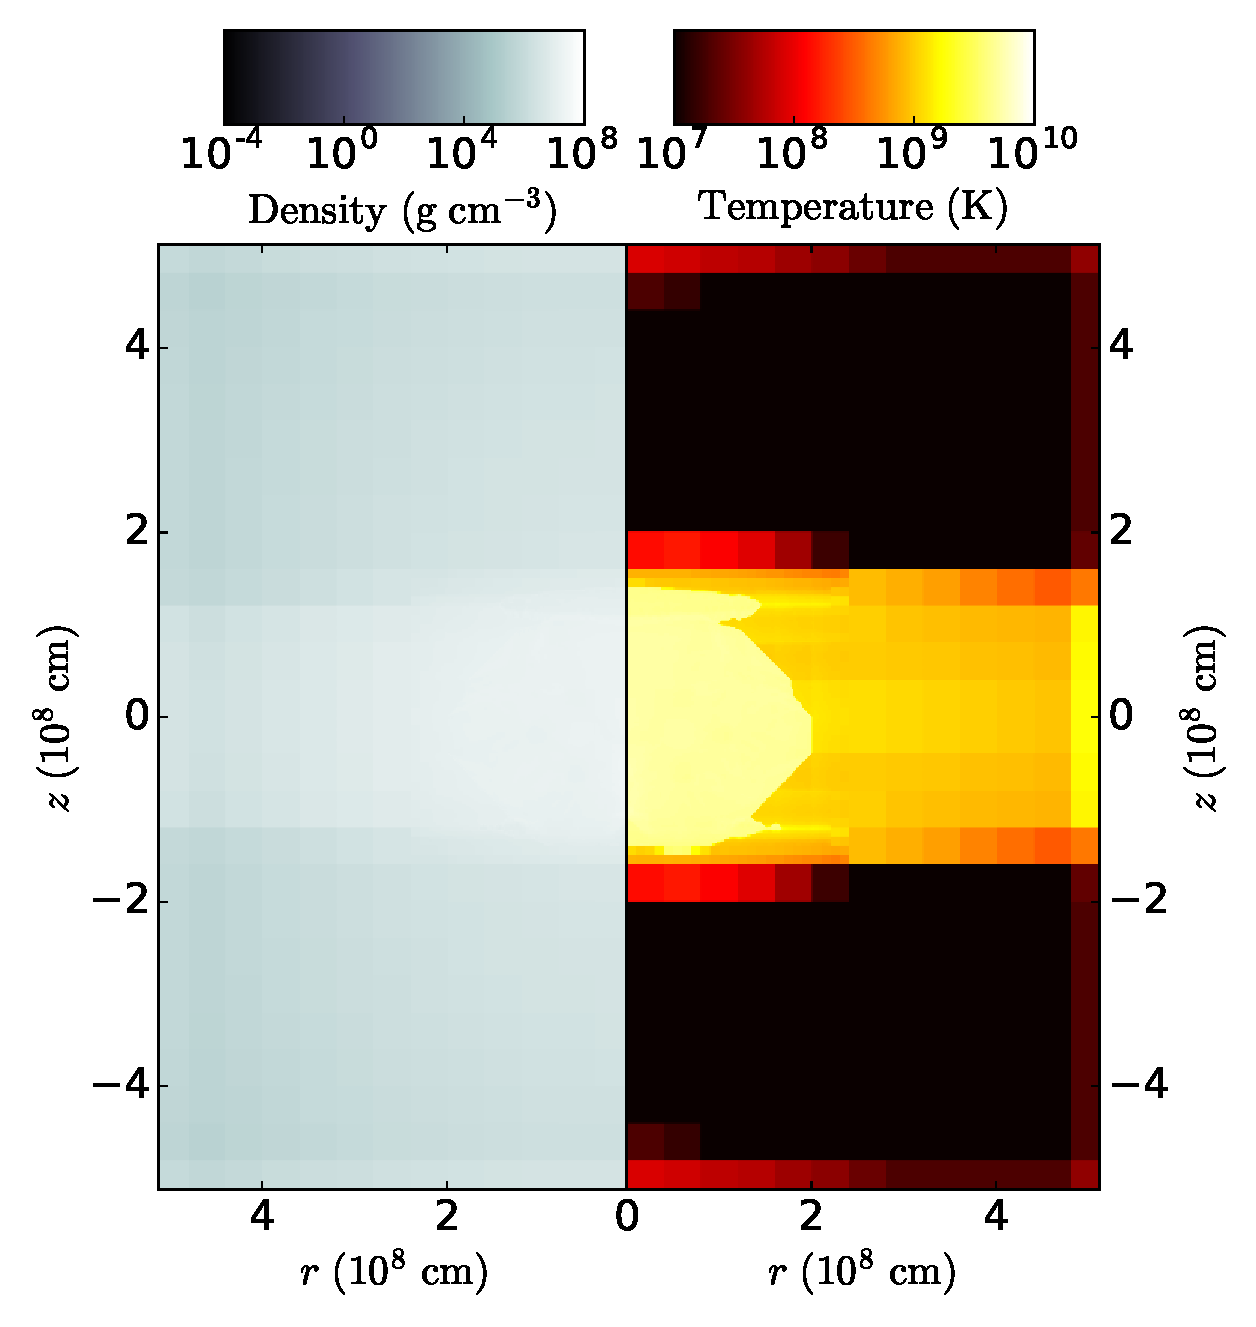
\includegraphics[scale=0.8]{{{plots/rho_T_slice_dxnuc_zoomed_r32_t_7.52}}}
  \caption[Initial detonation when refinement is based on burning rate]
          {Snapshot of the detonation formation (the bright region in the
           temperature field centered at $z = 0$). Refinement is based on the unstable
           burning criterion, with a maximal jump in refinement of 32 with
           respect to the coarse grid (effective resolution of 12.5 km).
           \label{fig:dxnuc_detonation}
          }
\end{figure}

However, the coarseness of the resolution means that there is an effective floor on any
detonation that is seeded by the coarse grid of 400 km. (Recall that the AMR criterion does
not take effect until after the unstable burning has begun.) If the actual scale for the
detonation formation is smaller than this, then the coarse grid hides the details of this
small-scale process, but in so doing may yield an inaccurate result for the nature of the
detonation. To study the effect of the small-scale burning physics, we swapped the adaptive
mesh refinement technique for a static one: maximally refine all zones within a radius of
200 km from the center, up to the specified maximum amount of refinement permitted on the
domain. The radius is chosen based on the finding of \citeauthor{kushnir:2013} that their
detonation occurs within that distance. The nickel production for this case is documented
in \autoref{fig:center_tagging_nickel}.

\begin{figure}[h]
  \centering
  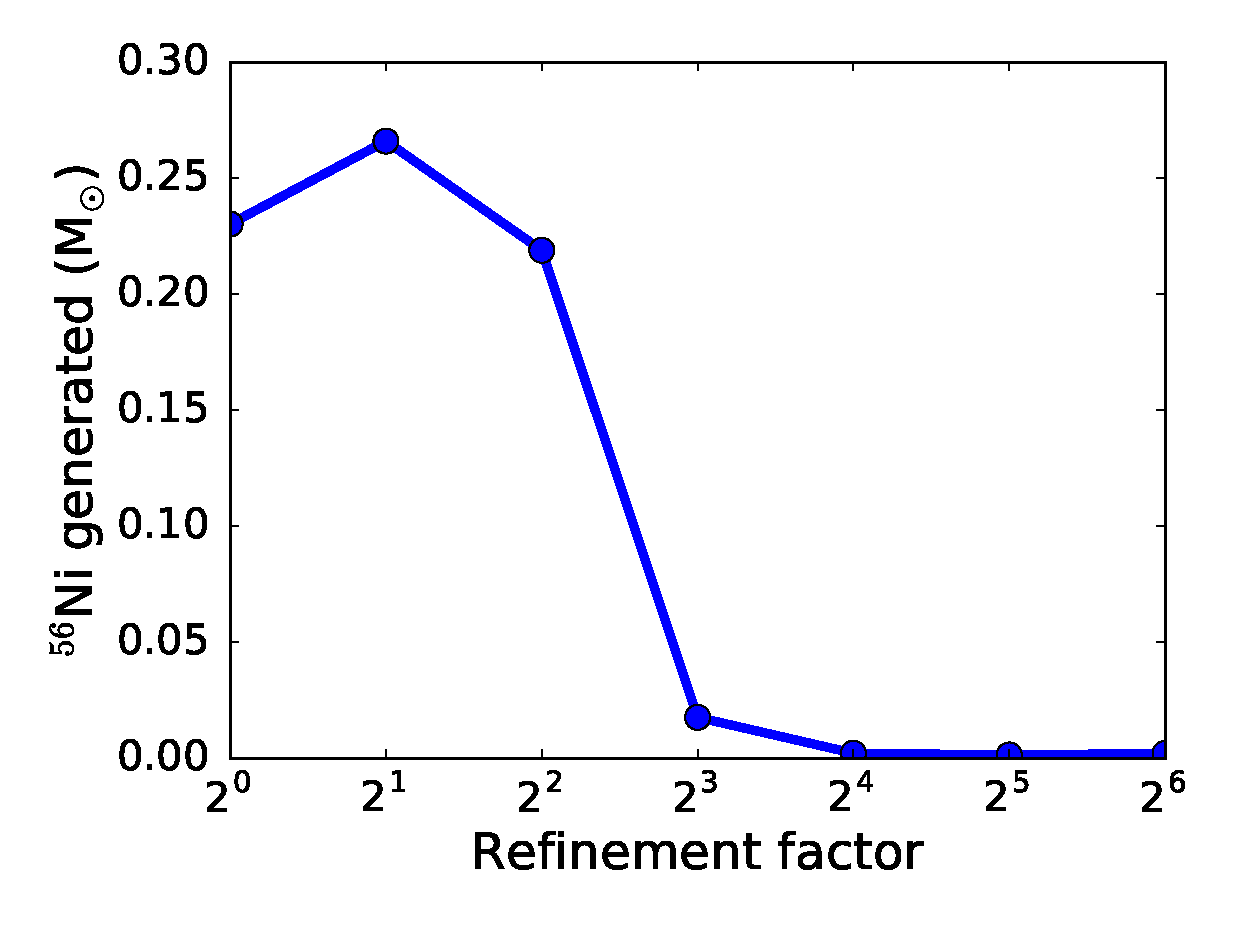
\includegraphics[scale=0.8]{{{plots/center_tagging_m_P_0.64_m_S_0.64}}}
    \caption[Nickel production as a function of static central refinement]
          {$^{56}$Ni production as a function of the maximum refinement factor
           relative to the coarse grid. Refinement is applied statically for
           all zones near the center of the domain.
           \label{fig:center_tagging_nickel}
          }
\end{figure}

The stark difference in this case, where at sufficient resolution very little nickel is generated,
is a consequence of the detonation occurring at a much earlier time ($\sim 6.7$ seconds). The high
density regions corresponding to the WD centers of mass are thus further away from the detonation,
so processing to NSE is largely precluded. Instead, there is efficient conversion of carbon into
silicon and sulfur material, but this event would look very different from a Type Ia supernova,
despite releasing enough energy to unbind the system. A snapshot of the inner 5\% of the domain is
shown in \autoref{fig:center_tagging_detonation} immediately after detonation has initiated. We find
that the early burning phase is characterized by a high temperature region at the center of the stalled
shock, which contains several local hotspots. The hotspots are not symmetrical with respect to $z = 0$
even though the initial problem setup is, which may reflect a lack of perfect symmetry in the hydrodynamics
algorithm we use or seeding by numerical error. The resolution in the detonation region is 6.25 km,
which is comparable to the resolution used by \citeauthor{kushnir:2013} in \flash. The major difference
between our result and theirs is their use of the suppressed burning mode. Even for a refinement factor
of 64, the sound-speed timescale $t_s$ is significantly longer than the energy injection timescale $t_s$
when the detonation forms, so there is evidence that this detonation is likely a numerical artifact.
The ratio of $t_s$ to $t_e$ trends downward with resolution at the initial detonation, and based on our
data would likely cross under unity when the resolution hits $\sim 1$ km. This lends support to the
basic conclusion that the nickel production is a strong function of when and where the detonation occurs,
with earlier detonations at small $z$ leading to lower amounts of nickel production. In this paradigm
we can then explain why the nickel production levels are at least within the same ballpark (a factor of
two compared to \citeauthor{kushnir:2013} and \citet{raskin:2010}) for the initially low resolution
runs that are tagged for refinement after the detonation occurs: the coarse size of the zones prevents
the detonation from occurring too early and too close to the center.

\begin{figure}[h]
  \centering
  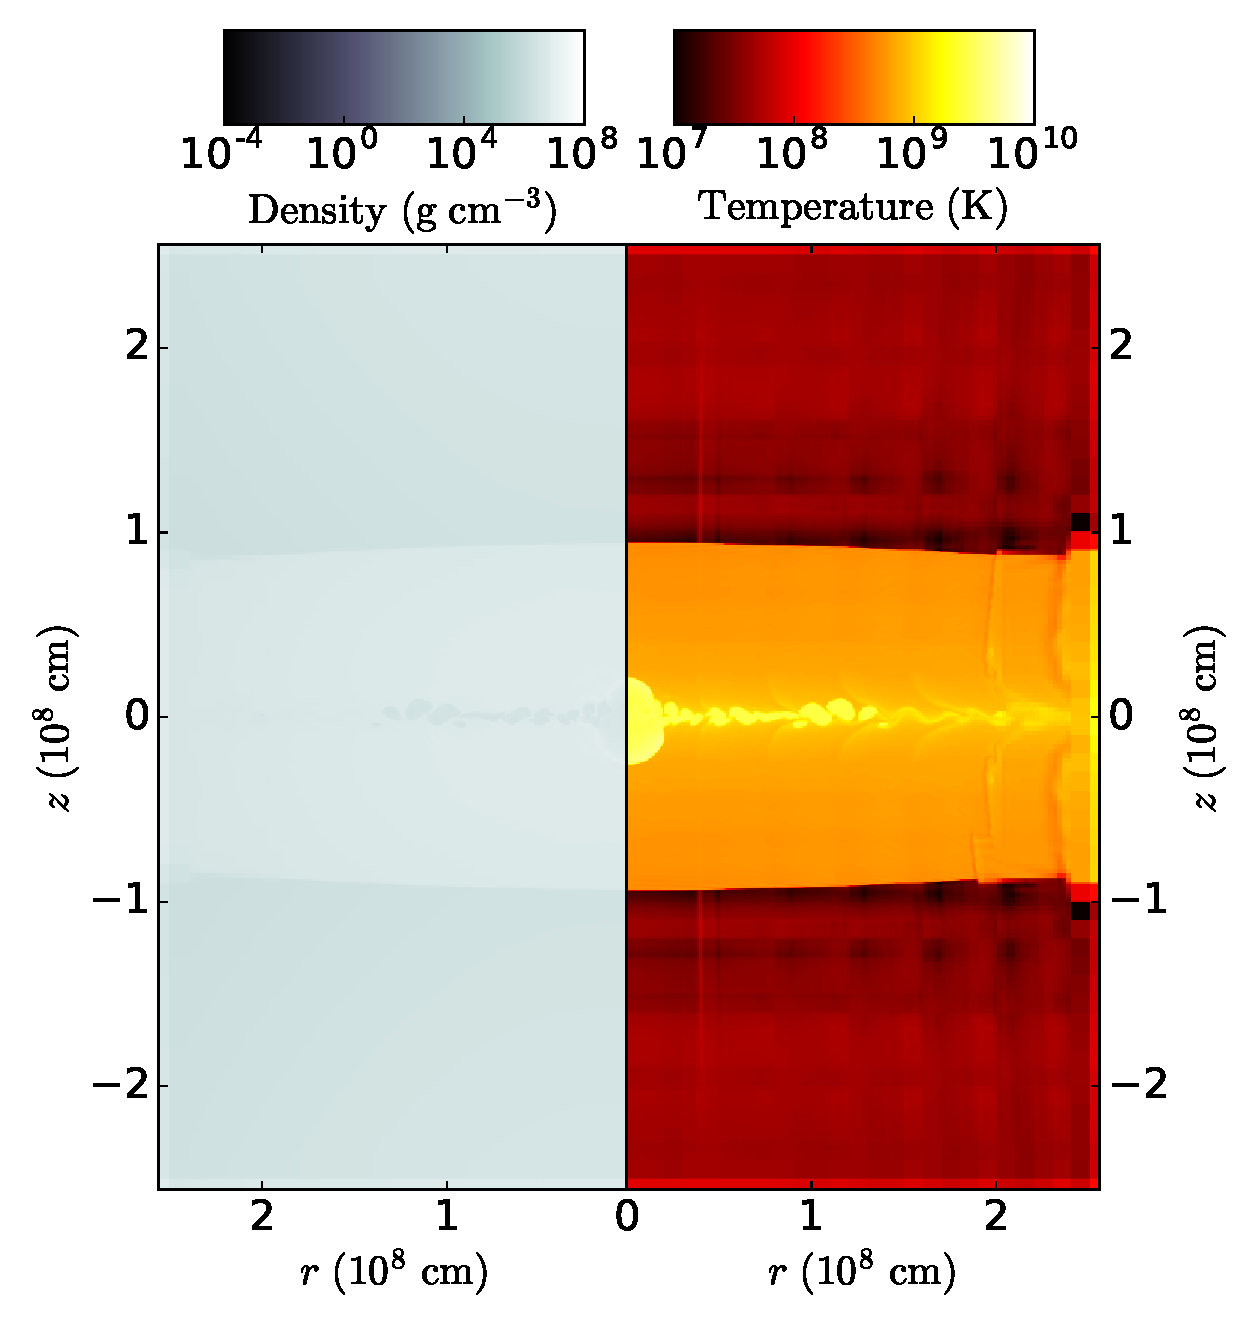
\includegraphics[scale=0.8]{{{plots/rho_T_slice_center_tagging_zoomed_r64_t_6.65}}}
  \caption[Initial detonation for static central refinement]
          {Snapshot of the detonation formation. The detonation is visible as a small,
           high-temperature region near $z = 0$ and $r = 0$. Refinement is applied
           statically for all zones near the center, with a maximal jump in refinement
           of 64 with respect to the coarse grid (effective resolution of 6.25 km).
           \label{fig:center_tagging_detonation}
          }
\end{figure}



\clearpage
\subsection{Gravitational Wave Signature}
\label{sec:collision_gravitational_waves}

While a typical merger event has a characteristic profile including a chirp and ringdown,
white dwarf collisions are noticeably distinct in their gravitational wave signatures, and
hence may be interesting targets for observation for future low frequency gravitational
wave detectors. The strain increases monotonically for a collision until impact,
instead of oscillating back and forth at a characteristic frequency as for mergers.
The main caveat for these events compared to events
such as neutron star mergers is that due to the event being inherently less energetic,
the typical distance scale on which we could observe a white dwarf merger or collision
is the size of our own galaxy, with extragalactic events being unlikely to be
detected, at least with the first generation of space-based gravitational wave
detectors.

\begin{figure}
  \centering
  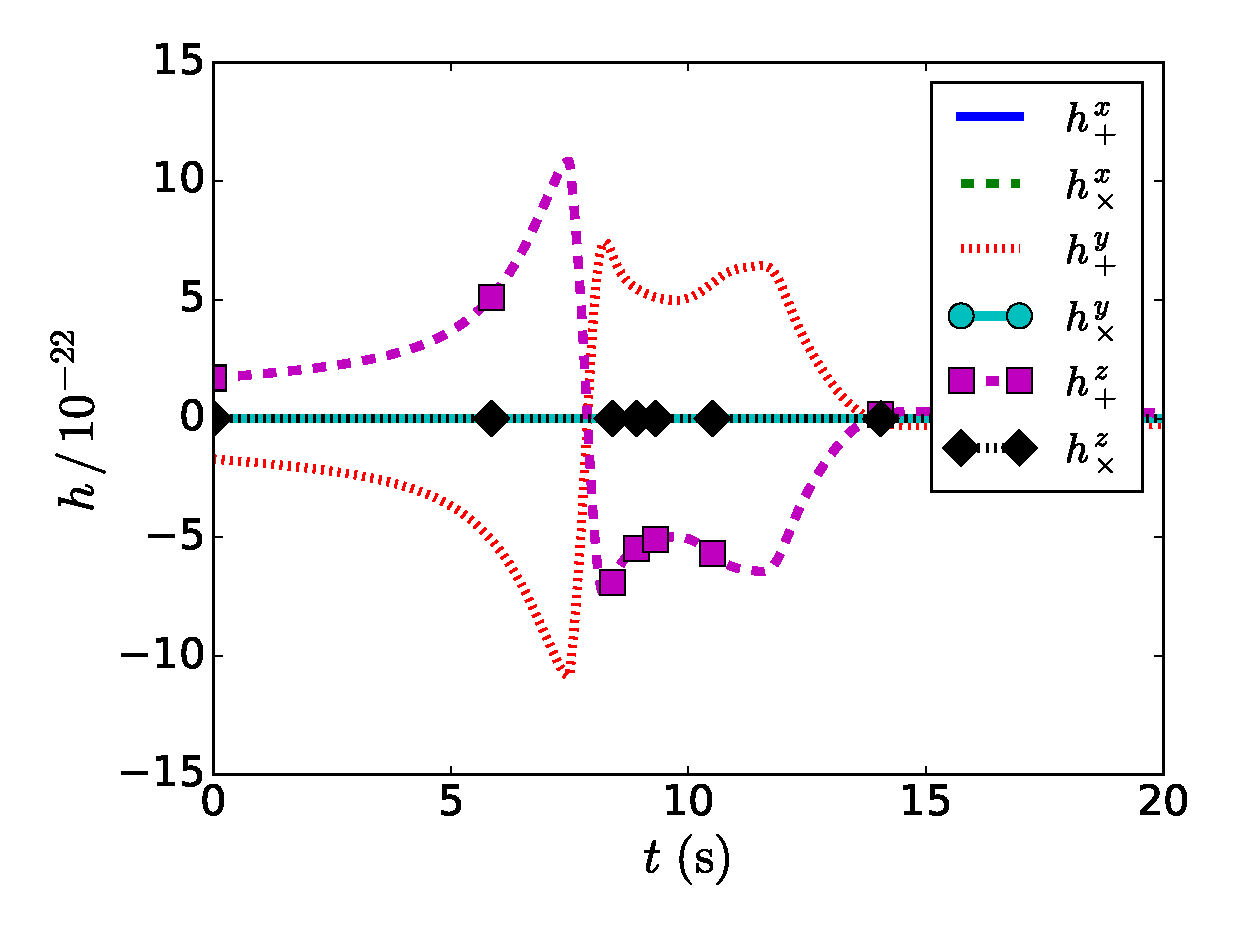
\includegraphics[scale=0.8]{plots/gw_signal_2D}
  \caption[Gravitational wave strain, head-on collision]
          {Gravitational wave strains for the head-on collision of two $0.64\ \msolar$
           white dwarfs. The strain is normalized to a source distance of 10 kpc.
           \label{fig:gw_signal_2D}}
\end{figure}

\autoref{fig:gw_signal_2D} is a plot of the gravitational wave strain for
the representative case of \autoref{sec:collision_parameters} ($M_P = 0.64\ \msolar$, $M_S = 0.64\ \msolar$, $b = 0$),
where we disabled the normal stopping criterion and let the simulation run until $t = 20$.
We show the $+$ and $\times$ polarizations for observers situated along the $x$, $y$,
and $z$ axes (for the 2D case, this corresponds to the $z$, $R$, and $\phi$ axes, respectively,
in the simulation) at the conventional distance of 10 kpc.
The shape of the profile agrees qualitatively with the gravitational wave signatures
predicted by \cite{loren-aguilar:2009:collisions} and \cite{garcia-senz:2013}.
\autoref{fig:gw_signal_3D} shows the strain prediction for a 3D collision event
with $M_P = 0.8\ \msolar$, $M_S = 0.6\ \msolar$, and $b = 0.8$. This mass combination
was chosen because \cite{loren-aguilar:2009:collisions} used the same combination for
gravitational wave signal prediction, but we cannot replicate the large impact parameter
they used on our simulation grid, so the detonation looks quite different than in their case.

\begin{figure}
  \centering
  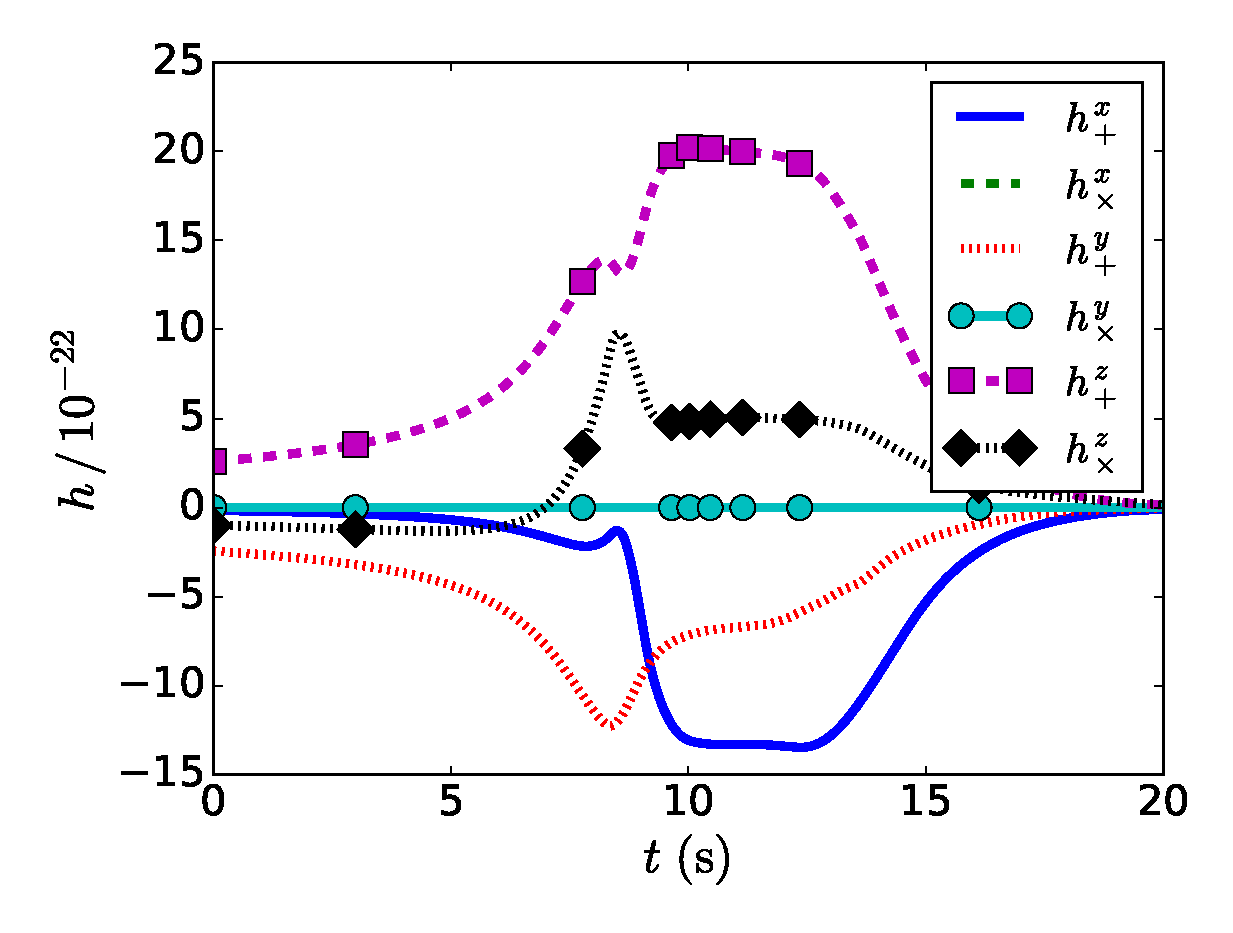
\includegraphics[scale=0.8]{plots/gw_signal_3D}
  \caption[Gravitational wave strain, off-center collision]
          {Gravitational wave strains for the off-center collision ($b = 0.8$) of
           $0.8\ \msolar$ and $0.6\ \msolar$ WDs. The strain is normalized to a
           source distance of 10 kpc.
           \label{fig:gw_signal_3D}}
\end{figure}



\newpage
\section{White Dwarf Mergers}
\label{sec:mergers}

In this section we turn to results from merger calculations. We focus specifically on
results from two cases: one where the secondary is just filling its Roche radius ($f_R = 1.0$);
and one where the secondary is already significantly overflowing its Roche radius ($f_R = 0.9$).
See \autoref{sec:initial_state:mergers} for a description of the initialization procedure; $f_R$
is defined as the ratio of the position of the location of the inner edge of the secondary (relative to
the origin) to the location where its inner edge would be equal to the location specified by the
effective Roche radius formula used in \autoref{eq:roche_radius}. In the former case mass transfer
begins slowly and steadily, while in the latter the binary orbit quickly decays and the system coalesces.

\subsection{Steady Mass Transfer}
\label{sec:mergers:stable}

For the case with $f_R = 1.0$, mass transfer begins immediately but at a slow and steady pace.
This would occur even if angular momentum was perfectly conserved, because the stars will deform
in response to the discrete nature of the grid and the tidal gravitational field of the other
star, and because the Roche lobe is not spherical, so some material will be jutting out of the
Roche lobe and become unbound from the secondary and fall onto the primary. For the case $f_R = 1.0$
we consider only the early mass transfer phase of the system so that we can understand the
convergence properties of the system and some basic properties of the mass transfer.

To determine the resolution needed to get the dynamics right, we repeated a test similar to that
of \autoref{sec:kepler}, running the same problem on our usual coarse grid ($n = 256$ zones
per spatial dimension) and on grids that have jumps by a factor of two or four ($n = 512$ or
$n = 1024$ effective zones per spatial dimension, respectively). In this section we choose
$M_P = 0.90\ \msolar$ and $M_S = 0.60\ \msolar$, which for $f_R = 1.0$ corresponds to an effective
Keplerian orbital period $T = 61$ seconds.

We ran the test in the four combinations corresponding to the inertial versus rotating frames
and the hybrid versus standard equations. We show most of the first orbit's worth of evolution
in \autoref{fig:merger_convergence_rot0_hybrid0} for evolution in the inertial frame using the
standard Euler equations, and in \autoref{fig:merger_convergence_rot1_hybrid1} for evolution
in the co-rotating frame using the angular momentum-conserving hybrid advection equations of
\autoref{sec:hybrid_advection}. The metric we use is the distance between the centers of mass
for the two stars.

\begin{figure}[h]
  \centering
  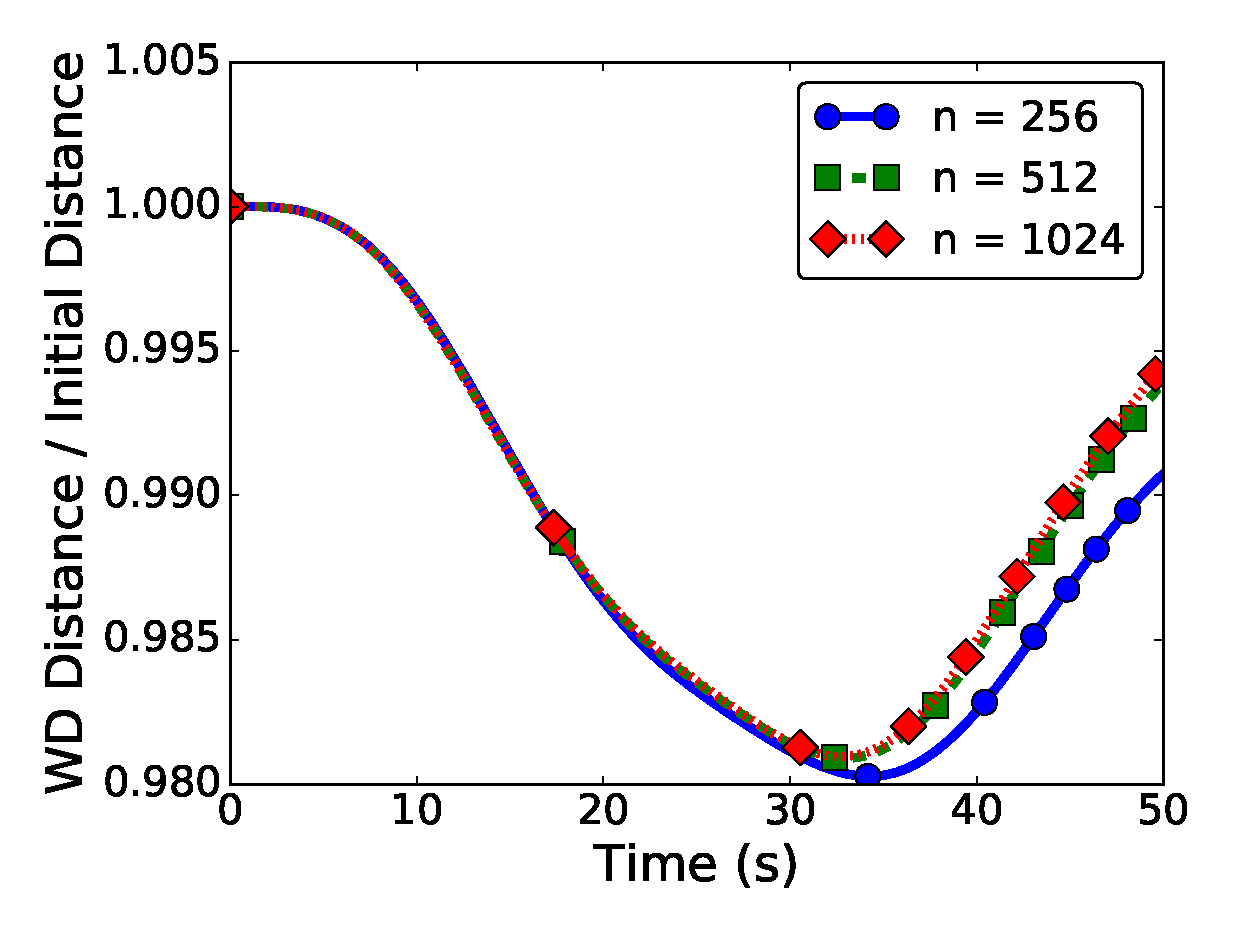
\includegraphics[scale=0.8]{{{plots/merger_convergence_m_P_0.90_m_S_0.60_roche_1.00_rot_0_hybrid_0}}}
  \caption[$f_R = 1.0$ convergence, inertial frame, standard equations]
          {Convergence properties of the $f_R = 1.0$ merger for the first 50 seconds (corresponding
           to approximately one full orbit) in the inertial frame with the standard equation set.
           The vertical axis is the distance of the stars normalized to their initial distance.
           The curves are labeled by the effective number of zones per dimension $n$.
           \label{fig:merger_convergence_rot0_hybrid0}
           }
\end{figure}

\begin{figure}[h]
  \centering
  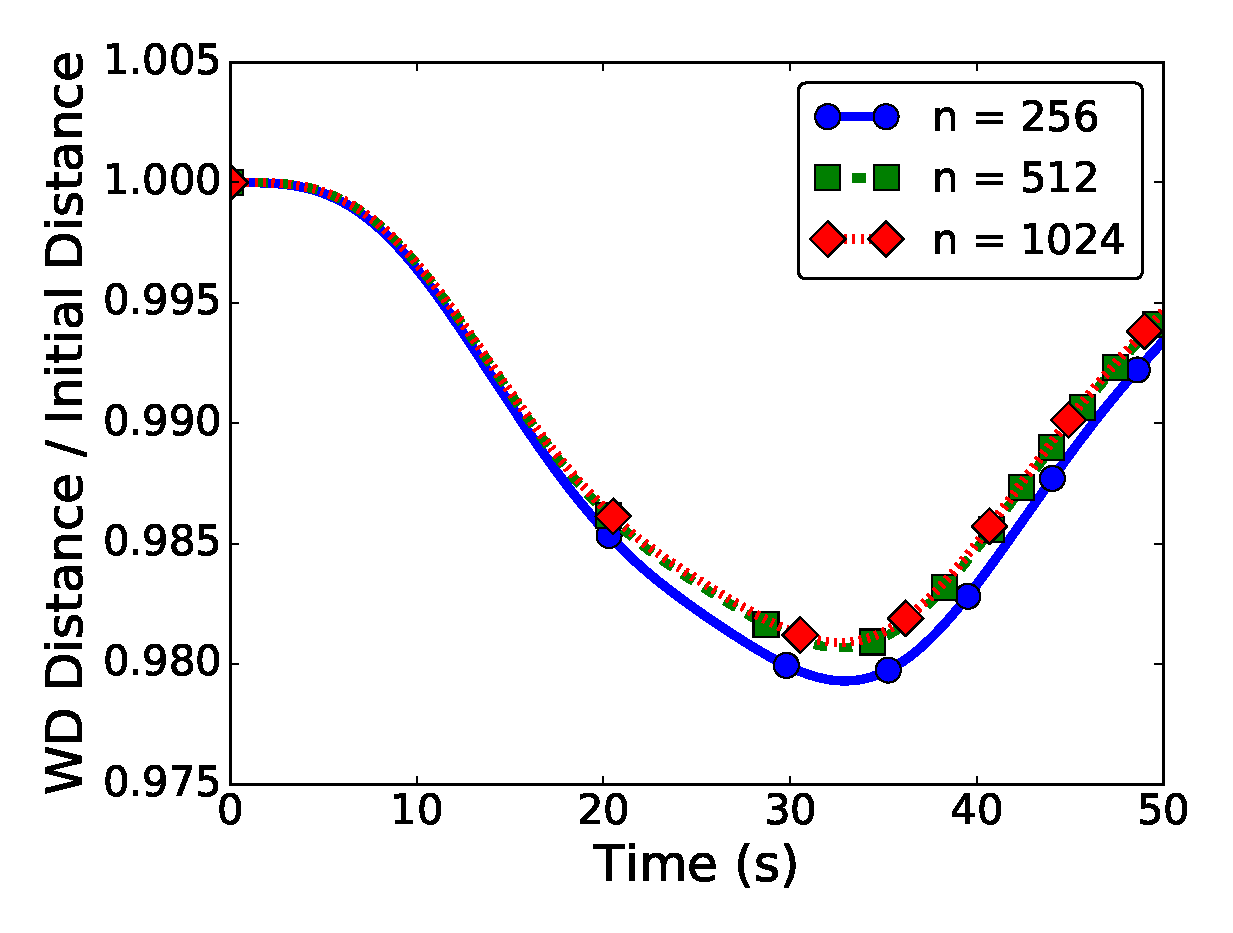
\includegraphics[scale=0.8]{{{plots/merger_convergence_m_P_0.90_m_S_0.60_roche_1.00_rot_1_hybrid_1}}}
  \caption[$f_R = 1.0$ convergence, rotating frame, hybrid equations]
          {Convergence properties of the $f_R = 1.0$ merger for the first 50 seconds (corresponding
           to approximately 80\% of one full orbit) in the rotating frame with the hybrid equation set.
           The vertical axis is the distance of the stars normalized to their initial distance.
           The curves are labeled by the effective number of zones per dimension $n$.
           \label{fig:merger_convergence_rot1_hybrid1}
          }
\end{figure}

The results confirm what we saw in \autoref{sec:kepler}: the grid that refines within the stars with
only a jump by a factor of two, with effective spatial resolution of 200 km, is sufficient to obtain
qualitative convergence and obtain fairly accurate quantitative results. We use results from that case
in the remaining plots in this section. The dynamical evolution between the two frames is qualitatively
pretty similar, which confirms the trustworthiness of the hybrid momentum formalism. The differences
between the two methods become more apparent upon looking at the angular momentum conservation in
\autoref{fig:merger_angular_momentum_comparison}. In the inertial frame, the system slowly leaks angular
momentum over time for either evolution method. Angular momentum changes are inevitable because of losses
or gains through the domain boundary (both hydrodynamic and due to the source terms) and because the
gravitational and rotational forces may not numerically be conservative in their effect on the angular
momentum (for example, this can happen due to gravity because of the non-zero error tolerance in the
solve for the potential). However, we have added to \castro\ the ability to directly track the amount
of mass, momentum, energy, and angular momentum lost off the domain boundary due to hydrodynamic fluxes,
and for the hybrid momentum evolution, the angular momentum changes are almost entirely dominated by
losses through the boundary, with less than 1\% of the angular momentum change due to effects other than
boundary losses. This implies that angular momentum within the stellar material itself is excellent.
That there is a steady loss of angular momentum on the full domain over this time period is an indication
of the fact that in the inertial frame, the stellar motion is constantly exciting ambient material through
hydrodynamic pressure waves as it plows through the ambient gas, driving periodic motions that prevent
the ambient material from reaching an equilibrium state (at least at this early time). As one would expect
for this mechanism, the amount of angular momentum lost through the grid boundary is nearly identical for
both the standard and hybrid evolutions. The difference is that the inertial frame has an additional source
of angular momentum loss which is over twice as large as the amount lost to the grid boundary. Consequently
the angular momentum conservation for the hybrid equations is actually far better than the plot first appears;
the total size of the change in the angular momentum is three orders of magnitude smaller for the hybrid equations
when this effect is accounted for. To illustrate this, in \autoref{fig:merger_angular_momentum_comparison_minus_grid_losses}
we show the same plot but with the domain boundary losses of angular momentum subtracted. This result confirms
that the hybrid advection technique does a much better job at its intended goal of angular momentum conservation.

\begin{figure}[h]
  \centering
  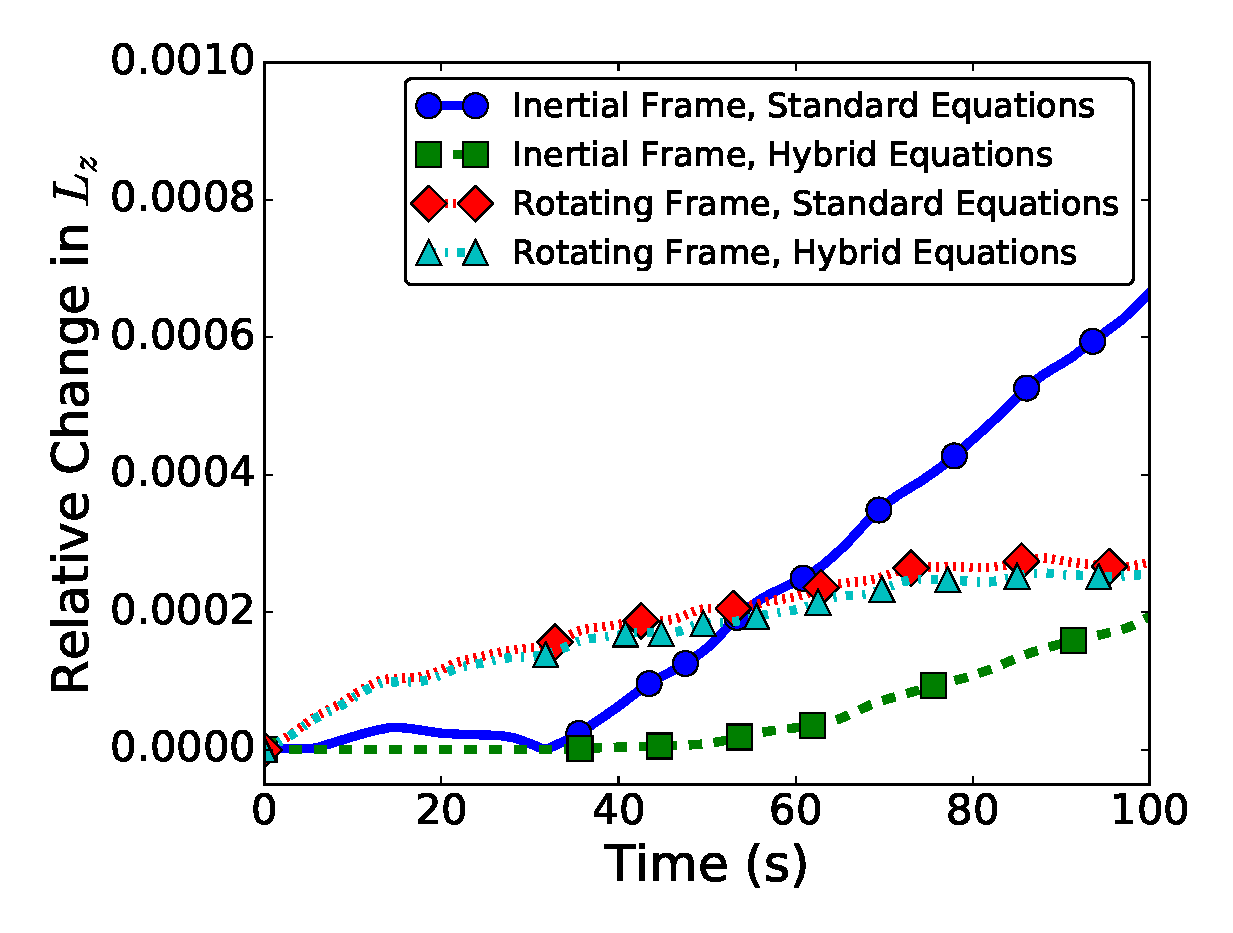
\includegraphics[scale=0.8]{{{plots/merger_angular_momentum_comparison_m_P_0.90_m_S_0.60_n_512}}}
  \caption[Angular momentum conservation for $f_R = 1.0$]
          {Angular momentum conservation error for the $f_R = 1.0$ merger for the first 100 seconds.
           The vertical axis is the absolute value of the change in the angular momentum relative to
           its initial value.
           \label{fig:merger_angular_momentum_comparison}
          }
\end{figure}

\begin{figure}[h]
  \centering
  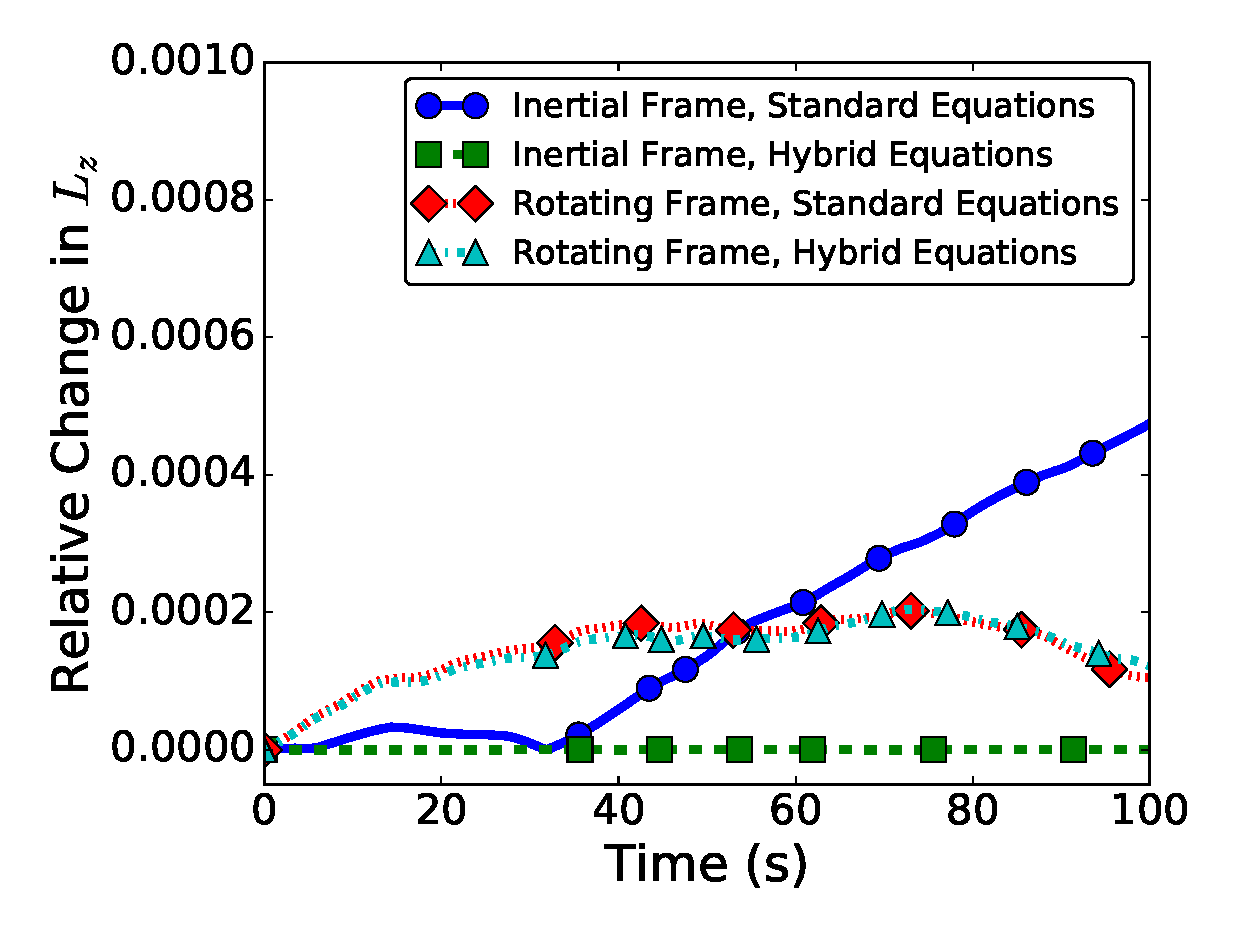
\includegraphics[scale=0.8]{{{plots/merger_angular_momentum_comparison_minus_grid_losses_m_P_0.90_m_S_0.60_n_512}}}
  \caption[Angular momentum conservation for $f_R = 1.0$, grid losses subtracted]
          {Same as \autoref{fig:merger_angular_momentum_comparison}, but losses through the
           domain boundary have been subtracted.
           \label{fig:merger_angular_momentum_comparison_minus_grid_losses}
          }
\end{figure}

The results of the rotating frame tell a slightly different story. In \autoref{fig:merger_angular_momentum_comparison},
we see that the angular momentum evolution is nearly identical in the rotating frame for both the standard
and the hybrid evolution. This is a consequence of the rotation source term having a property that the gravitational
source term does not. Momentum conservation for the latter is violated only to the extent that the cell-centered
gravitational acceleration does not exactly satisfy the Poisson equation (see \autoref{eq:momentum_discretization}
and the surrounding text), which is caused by small errors in the Poisson solve. By contrast, the rotation
source term as applied here is not numerically conservative, due mainly to the presence of the Coriolis term.
This could potentially be mollified by changing the way the rotation source term for momentum is applied, but
that is outside the scope of this work. However, the angular momentum eventually stabilizes (as we confirmed
by running the simulation a little longer), as the non-conservation effect here depends on the Coriolis
force, which is proportional to velocity and therefore becomes less important as the system reaches
a quasi-stable equilibrium. This is another application of the observation of \autoref{sec:kepler} that while
the rotating frame does a reasonable job of keeping the system stable against collapse, the Coriolis force
can wreak havoc if the system is far from equilibrium in the frame. We note in passing that \citet{byerly:2014}
have advocated a compromise approach where the variables are advected in a rotating frame but measured with
respect to the inertial frame. This has the nice effect of causing the Coriolis term to drop out of the
angular momentum equation in the hybrid equation set, so it is a promising avenue for future work.

The final quantity we look at is the mass of the stars over this time period, shown in \autoref{fig:steady_mass_transfer}.
The mass of the secondary declines at a steady secular rate of approximately $2 \times 10^{-5}\ \msolar\ \text{s}^{-1}.$
This mass loss is modulated by a periodic oscillation of the stars around their quasi-static orbital distance,
a consequence of not starting the stars exactly in equilibrium.
This mass loss rate is such that if it were maintained linearly, the secondary would disrupt completely in
approximately 100 orbits. Of course, this estimate is an upper bound, as white dwarfs expand when
they lose mass, making escape of material through the Roche lobe surface easier, amplifying the mass loss
in a non-linear feedback loop (see the discussion in \citet[Section 2]{dan:2011} for an overview of the
physics related to mass transfer stability). Nevertheless, this estimate is far longer than the $\sim 1$
orbital period that this system lasts in \citet{dan:2011}, and more in keeping with the $\sim 30$ orbital
periods of mass transfer they obtained when starting from equilibrium initial conditions. Why is there
such a stark difference? It is true that an AMR code is better equipped to resolve small levels of mass transfer
than a SPH code that uses equal-mass particles because the density in a zone can take effectively
any value, while for the SPH code mass transfer occurs in more discrete chunks corresponding to the motion of
particles on the domain. Nevertheless, even a small number of SPH particles would be sufficient to
resolve the mass transfer rate we observe in our simulation. The dominant effect actually comes from
the fact that our initial WD distance is about 15\% larger. The cause of this is found in
a relatively obscure place: the use of Coulomb corrections in the equation of state. We enable the Coulomb
corrections in the Helmholtz equation of state, and for a given stellar mass the Coulomb corrections cause
the star to be more compact (the central density becomes about 10\% higher), with a smaller radius. But since,
like \citeauthor{dan:2011}, we selected the initial WD distance to be based on the WD radius, and the Roche lobe
size does not depend on the WD radius, the effect of enabling the Coulomb corrections is to make the distance
implied by the Roche lobe-based algorithm to be larger. While \citeauthor{dan:2011} do not explicitly state whether
they use the Coulomb corrections, we obtain nearly exact agreement with the initial WD distance they report
if we disable the Coulomb corrections. (Note that there can be small differences in the reported radius
even for identical equations of state since the initial radius depends on what cutoff density is used in
computing the initial one-dimensional stellar model.) Consequently, less of our star is outside the
Roche lobe than theirs is, so our mass transfer is much steadier.

\begin{figure}
  \centering
  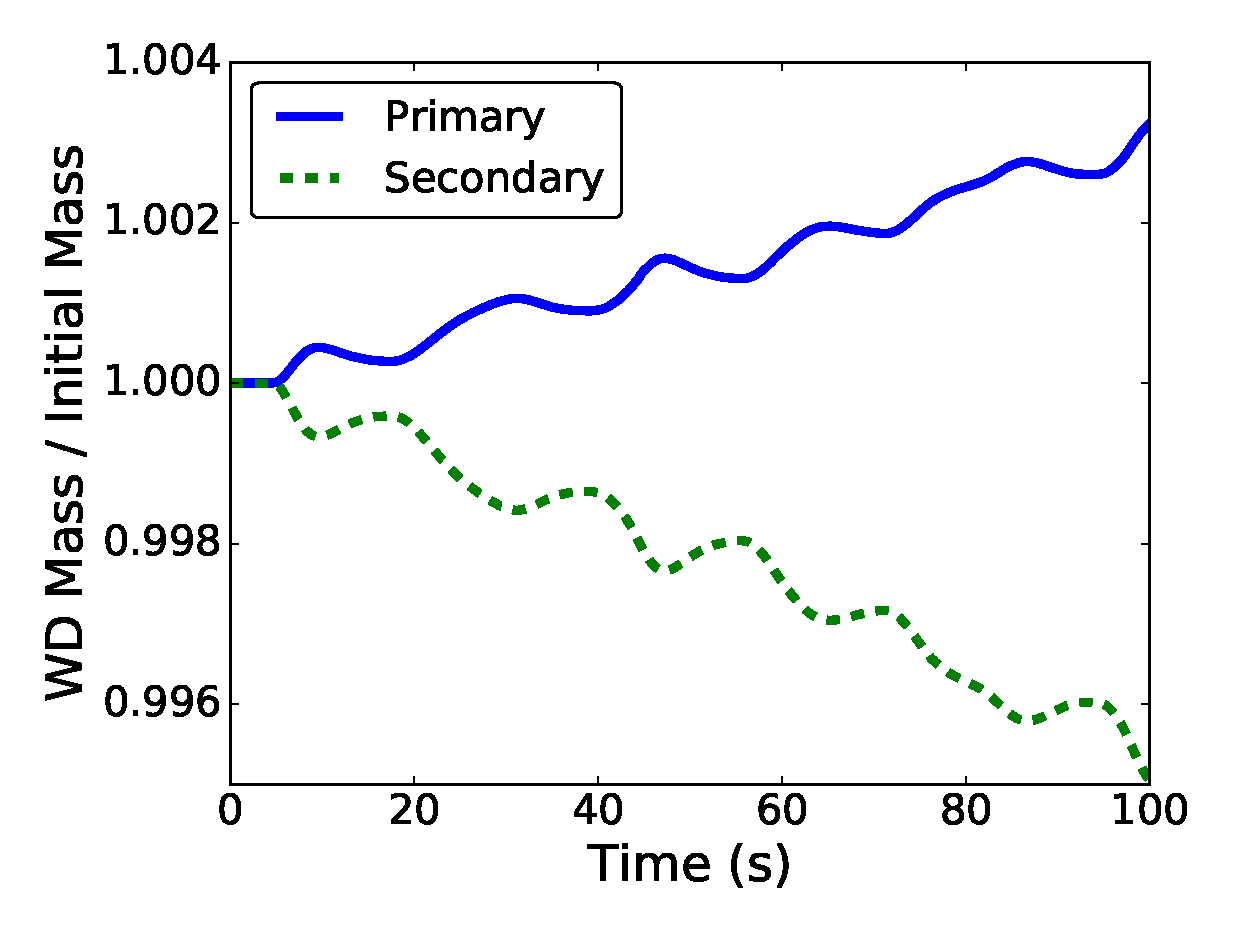
\includegraphics[scale=0.8]{{{plots/merger_masses_m_P_0.90_m_S_0.60_roche_1.00_rot_0_hybrid_1_n_512}}}
  \caption[Stellar masses, steady mass transfer case]
          {Mass of the primary ($M_P = 0.9\ \msolar$) and secondary ($M_S = 0.6\ \msolar$)
           stars for $f_R$, normalized to their initial masses.
           The evolution is done in the inertial frame with the hybrid equation set.
           \label{fig:steady_mass_transfer}
          }
\end{figure}

We agree with \citeauthor{dan:2011} that equilibrium initial conditions can play an important role in
determining the subsequent mass transfer, and that the cause of this is largely due to tidal
deformation of the stars and also that the equilibrium simulation starts mass transfer at a
larger radius. The upshot here though is that we can use a larger initial distance even without
the equilibrium conditions; $f_R = 1.0$ is not clearly the uniquely correct choice for
``approximate`` initial conditions, as resolvable mass transfer can occur even at larger $f_R$.
Due to this, and also because equilibrium initial conditions are themselves idealized cases
(and it is not even fully clear whether binary WDs do become completely tidally locked on the
relevant evolution timescale), a full understanding of the effect of the initial conditions
on the outcome of the merger process requires comparing merger simulations that realize more
fully the possible initial conditions for these systems.



\subsection{Unsteady Mass Transfer}
\label{sec:mergers:unstable}

Here we briefly consider results for mergers that are immediately unstable to mass transfer.
Because of the above caveats about the initial conditions, these tests should not be considered
representative of how the mergers would physically occur.
Future work will compare these results against more accurate initial conditions.

\subsubsection{Unequal Mass Merger}
\label{sec:mergers:unstable:unequal}

To obtain unstable mass transfer on a short simulation timescale, we repeated the test of
\autoref{sec:mergers:stable}, for a $0.9\ \msolar$ primary and $0.6\ \msolar$ secondary, with
$f_R = 0.9$, so that the stars are 10\% closer to each other. This
is a very significant change, as now much of the secondary is overflowing its Roche lobe and
substantial mass transfer begins immediately; the mass transfer rate reaches
$10^{-3}\ \msolar\ \text{s}^{-1}$ in under five seconds. We ran the test with an effective
$512^3$ zone, 200 km resolution for the hybrid advection case only, in both the inertial and
rotating frames. Snapshots of the evolution in both frames are found in
\autoref{fig:unsteady_mass_transfer_unequal_inertial} and
\autoref{fig:unsteady_mass_transfer_unequal_rotating}, respectively. The initial
Keplerian orbital period for this system is 52 seconds, so the timescale for
complete disruption of the secondary is about three orbital periods.

The temperature peaks at around $10^9$ K during this merger, which happens around $t = 135\ \text{s}$
when the flow of stellar material onto the primary WD's surface is near its height. This occurs
in material with densities approaching $10^6\ \text{g cm}^{-3}$, so the conditions are clearly ripe
for significant levels of thermonuclear burning. In followup simulations we will enable reactions
to see what effect they have. However, two important caveats are worth considering. First, the mass
transfer phase here is more violent than it would be for different initial conditions, so the
burning here is not necessarily representative for all cases. Second, the burning in this type of system
may be susceptible to the same type of burning instability that afflicts the collisions, so any detonation
obtained at this low resolution should be viewed with significant caution. We can make progress on this
by adding significant refinement at the impact point, though.

The conservation properties are similar as for the steady mass transfer phase (for the following, the
data comes from the inertial frame run). At $t = 150$ s, after complete disruption has occurred, the
magnitude of the total angular momentum on the domain has decreased by about 11\%, but this is mainly
due to mass leaving the domain as it is flung outward by the tidal tail that develops. When this is
accounted for, the angular momentum loss due to other sources is about 0.02\% of the initial angular
momentum. Conservation of linear momentum is not quite as good, but still respectable.
A good proxy for this is to look at where the system center of mass is. At $t = 150$ s,
$x_{\text{COM}} = 4.6 \times 10^7\ \text{cm}$ and $y_{\text{COM}} = 9.8 \times 10^7\ \text{cm}$. Recall that
the effective resolution is 200 km, so this is equivalent to the system center moving a few zones away
from the center over the course of the evolution. The center of mass usually stays a little better
localized in the case where we evolve the linear momentum equations. About 0.7\% of the initial energy
is lost, half of which is accounted for by hydrodynamic fluxes off the domain.

\begin{figure}[h]
  \centering
  \includegraphics[scale=0.61]{{{plots/merger_time_series_m_P_0.90_m_S_0.60_roche_0.90_rot_0_hybrid_1_n_512}}}
  \caption[Density evolution, unequal mass merger ($f_R = 0.90$, inertial frame)]
          {Density evolution for the unequal mass merger starting with $f_R = 0.9$.
           The view is a slice plot of the $z = 0$ plane. The evolution is in the
           inertial frame. For visual clarity we show only the inner 75\% of the domain.
           The simulation time is displayed in the upper left corner of each pane.
           \label{fig:unsteady_mass_transfer_unequal_inertial}
          }
\end{figure}

\begin{figure}[h]
  \centering
  \includegraphics[scale=0.61]{{{plots/merger_time_series_m_P_0.90_m_S_0.60_roche_0.90_rot_1_hybrid_1_n_512}}}
  \caption[Density evolution, unequal mass merger ($f_R = 0.90$, rotating frame)]
          {Density evolution for the unequal mass merger starting with $f_R = 0.9$.
           The view is a slice plot of the $z = 0$ plane. The evolution is in the
           rotating frame. For visual clarity we show only the inner 75\% of the domain.
           The simulation time is displayed in the upper left corner of each pane.
           In this plot we have not transformed back to the inertial frame. 
           \label{fig:unsteady_mass_transfer_unequal_rotating}
          }
\end{figure}

\autoref{fig:unsteady_gw_signal_unequal} shows the gravitational wave signal for this event. The
signal has the expected characteristics for such an event when viewed perpendicular to the
rotation axis: initially, the signal has a constant amplitude and an oscillation period equal
to half the orbital frequency. As significant mass transfer sets in, the frequency increases
because of rapid coalescence, and then the system eventually relaxes to an equilibrium (the ringdown phase). 

\begin{figure}[h]
  \centering
  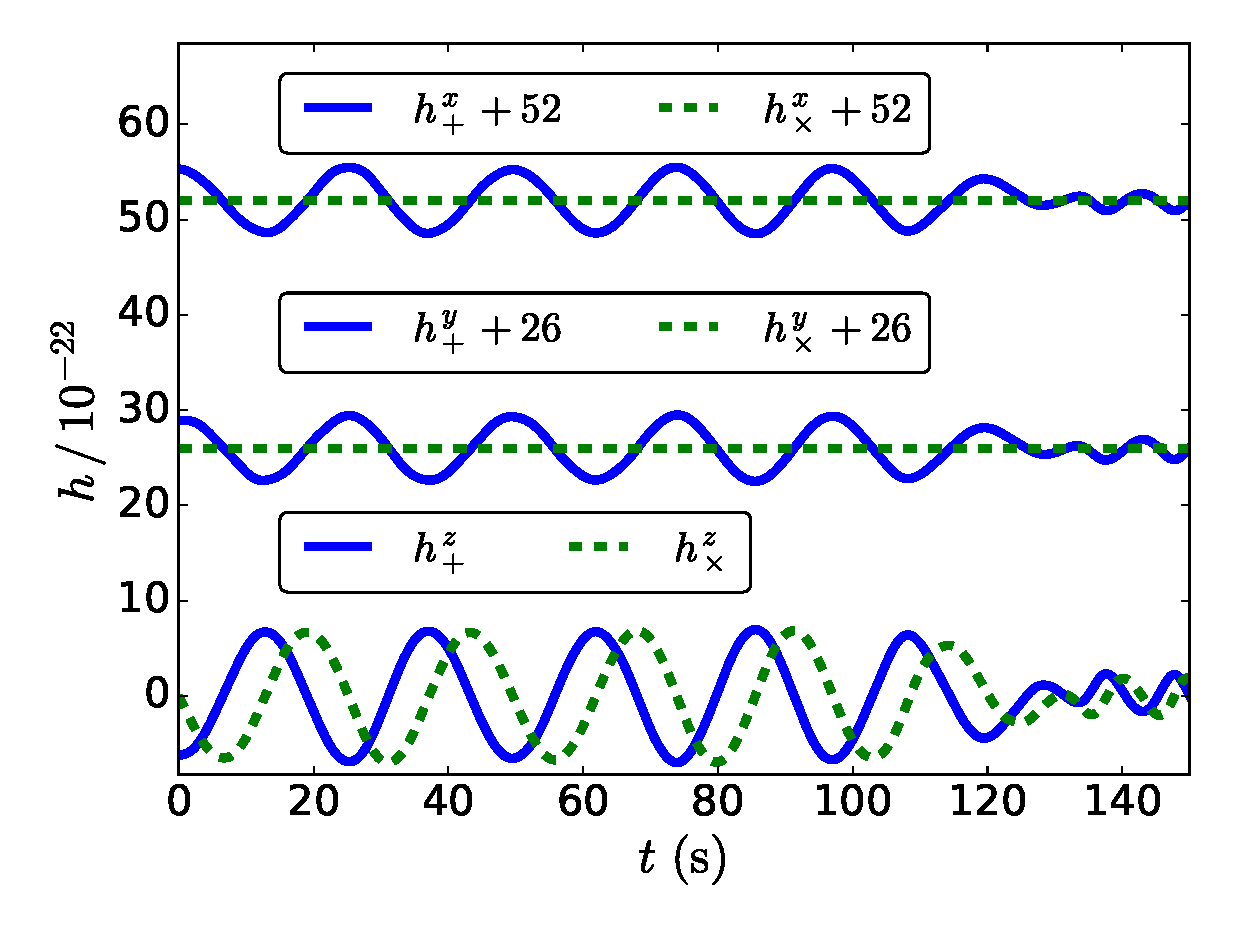
\includegraphics[scale=0.8]{{{plots/merger_gw_signal_m_P_0.90_m_S_0.60_roche_0.90_rot_0_hybrid_1_n_512}}}
  \caption[Gravitational wave signal, unequal mass merger ($f_R = 0.90$)]
          {Gravitational wave strain for the unequal mass merger starting with $f_R = 0.9$.
           From top to bottom, we show the $+$ and $\times$ polarizations for observers
           at 10 kpc along the $x$, $y$, and $z$ axes respectively.
           \label{fig:unsteady_gw_signal_unequal}
          }
\end{figure}



\clearpage
\subsubsection{Equal Mass Merger}
\label{sec:mergers:unstable:equal}

Equal-mass mergers are maximally unstable against mass transfer so they provide a
limiting case for how violent the coalescence phase is.
We use two $0.9\ \msolar$ mass stars for the simulation shown here, again with $f_R = 0.9$
and an effective 200 km resolution. The inertial frame evolution is displayed in
\autoref{fig:unsteady_mass_transfer_equal_inertial} and the rotating frame evolution is
displayed in \autoref{fig:unsteady_mass_transfer_equal_rotating}. The initial Keplerian
orbital period for this system is 24 seconds, so the coalescence has essentially completed,
leaving a single merged remnant, within two orbital periods. The conservation properties
are very similar to those discussed in \autoref{sec:mergers:unstable:unequal}. The
corresponding gravitational wave signal is shown in \autoref{fig:unsteady_gw_signal_equal}.

\begin{figure}[h]
  \centering
  \includegraphics[scale=0.61]{{{plots/merger_time_series_m_P_0.90_m_S_0.90_roche_0.90_rot_0_hybrid_1_n_512}}}
  \caption[Density evolution, equal mass merger ($f_R = 0.90$, inertial frame)]
          {Density evolution for the equal mass merger starting with $f_R = 0.9$.
           The view is a slice plot of the $z = 0$ plane. The evolution is in the
           inertial frame. For visual clarity we show only the inner 75\% of the domain.
           The simulation time is displayed in the upper left corner of each pane.
           \label{fig:unsteady_mass_transfer_equal_inertial}
          }
\end{figure}

\begin{figure}[h]
  \centering
  \includegraphics[scale=0.61]{{{plots/merger_time_series_m_P_0.90_m_S_0.90_roche_0.90_rot_1_hybrid_1_n_512}}}
  \caption[Density evolution, equal mass merger ($f_R = 0.90$, rotating frame)]
          {Density evolution for the equal mass merger starting with $f_R = 0.9$.
           The view is a slice plot of the $z = 0$ plane. The evolution is in the
           rotating frame. For visual clarity we show only the inner 75\% of the domain.
           The simulation time is displayed in the upper left corner of each pane.
           In this plot we have not transformed back to the inertial frame. 
           \label{fig:unsteady_mass_transfer_equal_rotating}
          }
\end{figure}

\begin{figure}[h]
  \centering
  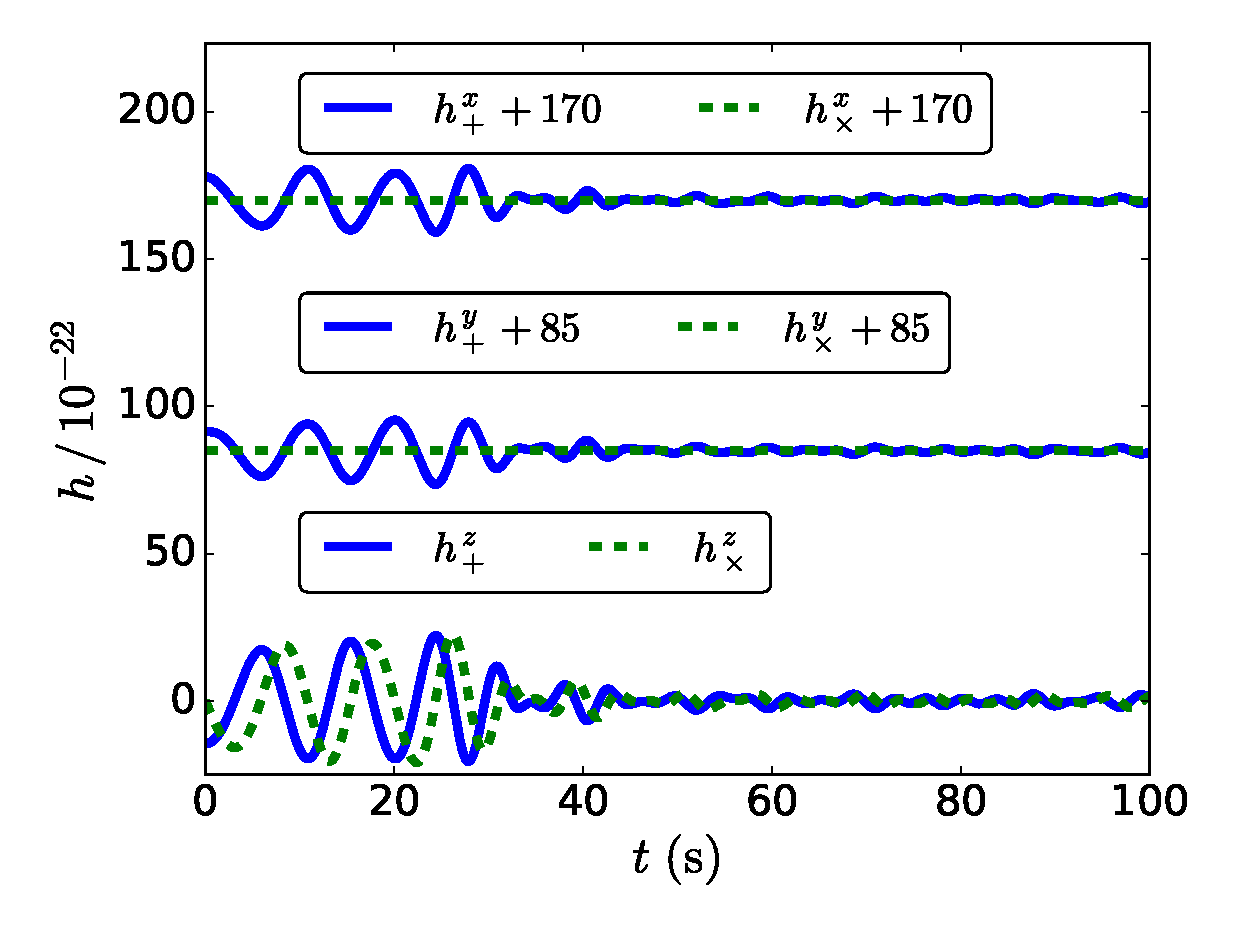
\includegraphics[scale=0.8]{{{plots/merger_gw_signal_m_P_0.90_m_S_0.90_roche_0.90_rot_0_hybrid_1_n_512}}}
  \caption[Gravitational wave signal, equal mass merger ($f_R = 0.90$)]
          {Gravitational wave strain for the unequal mass merger starting with $f_R = 0.9$.
           From top to bottom, we show the $+$ and $\times$ polarizations for observers
           at 10 kpc along the $x$, $y$, and $z$ axes respectively.
           \label{fig:unsteady_gw_signal_equal}
          }
\end{figure}



\clearpage
\section{Conclusions}
\label{sec:conclusion}

Reacting, self-gravitating, hydrodynamic flows pose many interesting computational challenges,
in both computational performance and numerical accuracy. There are outstanding questions of
numerical stability both in the pure hydrodynamics (\autoref{sec:galileo}) and in the
reactions (\autoref{sec:unstable_burning}), and fundamental questions about how to
correctly couple hydrodynamics, gravity, and reactions together given that they operate on
fundamentally different timescales and have very different effects on the nature of the
fluid flow. We have seen that failure to pay careful attention to this coupling can lead
to devastating effects like violation of energy and angular momentum conversation and
numerically seeded thermonuclear detonations. All of these effects, and more, make it very
difficult to state with confidence whether a given system is likely to correspond to an
observed astrophysical explosion based on simulation results. The point of this dissertation
is therefore not to make definitive statements about the extent to which double white dwarf
systems contribute to particular events like Type Ia supernovae, but rather to answer the
question of when we can trust the results of simulations of these events, and to suggest
computational techniques that improve the legitimacy of these simulations. We hope that our
work instills the point that one should not simply download a research-grade simulation code
and use it without understanding the impact of the various choices made in the software.

For merger simulations, we found that the most important stumbling blocks to trustworthy
simulations are the non-conservation of energy (due to the coupling of the gravitational
and rotational forces to the hydrodynamics), and the non-conservation of angular momentum.
Both can play very important effects on the long-term stability of a binary system, and
also shape the mass transfer phase. It must be emphasized that conservation of angular momentum
and energy are not always obviously the right things to enforce in a simulation; sometimes
small violations of these properties can be justified if it means more accurate thermodynamics
or hydrodynamics on smaller timescales. But if what we are interested in is the long-term
stability of the flow, then paying attention to the conservation properties is paramount.
While an angular-momentum-conserving approach (say) may introduce non-physical artifacts into
the simulation that cause the stellar flow to be inaccurate, they are certainly less disastrous
than the alternative of ignoring conservation, as this leads to spurious coalescence.
We have found that the use of a hybrid advection technique that advects angular and radial
momentum (and therefore conserves the former hydrodynamically) rather than linear momenta
can be very helpful in improving the conservation properties for angular momentum. And for
conservation of energy, we found that explicitly constructing the source terms in a conservative
manner (for example, by evaluating source terms at zone edges where hydrodynamic fluxes actually
occur rather than zone centers) permits reasonable conservation of energy on much longer
timescales than was previously possible in our simulations. Future work on the mergers can then
pay attention to the construction of accurate and physically meaningful initial conditions,
confident that the issues with the subsequent evolution have been well-characterized.

Collisions of white dwarfs are less challenging from the perspective of the gravity and
rotation forces, but they easily make up for it in their demand for accurate evolution of
the nuclear reaction source term. In this work we have characterized two effects that
play a major role on the accuracy of these simulations. First, the operator splitting
coupling the hydrodynamics and reaction steps introduces non-physical artifacts due to
the feeding of fresh, unburned material into the burning region occurring in staggered,
discrete steps rather than continuously. We have shown that this can have a very large
effect on the accuracy of a simulation and that using a timestep limiter that accounts
for this can help limit the effect. However, we also showed that the amount of limiting
needed to achieve a converged simulation is prohibitively large. Future work should focus
on more accurate methods of coupling these two updates. Second, low spatial resolution
introduces the possibility of numerically seeded detonations that bear no resemblance
to what a physical detonation would look like. However, the correct spatial resolution needed
to fully avoid this possibility is also quite restrictive (note though that higher
spatial resolution automatically leads to smaller timesteps due to the CFL stability
criterion, which may capture some of the temporal resolution effect just described, so
even adding some resolution will often be worth it even if the full resolution cannot
be achieved). Furthermore, even adaptive mesh refinement that targets this effect
can miss a detonation that begins before the refinement has kicked in, and we have shown
that adding resolution can actually make the result look even more incorrect than
using low resolution (though this really says that the coarse resolution simulations are
simply not qualitatively correct, and the fact that they get a plausible answer for
the head-on collision problem is to some extent a consequence of the nature of the problem).
Future work should be focusing on efforts that add resolution in the places where it is
needed rather than resorting to approximate workarounds, but the computational resources
demanded by this will make it difficult to perform large studies of the collision
parameter space in three dimensional simulations. At any rate, it is clear that the story
of explosive burning in hydrodynamics simulations is far from over. This has relevant
consequences even for the question of whether the inspiral mergers can lead to detonations,
because simulations that have found detonations in these mergers typically have employed
spatial resolutions that are far too low to understand the small-scale burning activity.
It is quite likely that if the requisite resolution were to be added, the location and
time of any detonations may change substantially, or even reveal the detonation itself
to be spurious.

More broadly, this dissertation is intended to emphasize that the challenges of
accurate large-scale hydrodynamical simulations require a rigorous understanding of
the limitations of these simulations and a serious approach to reproducibility. Much
of the challenge in comparing results from different simulation methods and academic
groups is the lack of a common language in which to perform such comparisons, and often
a lack of motivation to be fully open about the details of the computational methods used
make it quite difficult to reproduce the work of others. We hope that by publishing fully
the software we have used for the generation and analysis of our simulation results, we
are encouraging others to examine our approach and challenge the assumptions we make, in
addition to the more prosaic but crucially important issues like finding programming errors.
The only way that this can be achieved is by throwing as much sunlight on what we are doing
as is possible, so that others who seek to replicate our work do not have much trouble in
understanding what we did. Even if we ignore the broader concerns about the impact of
study replicability, there is a simple reason why publishing of the software is important:
it is not feasible or desirable to list every minor code choice in a research document.
Publishing the software allows the researcher to safely decide what details are relevant
to include in the text of a manuscript, and what details are best left for the documentation
of the software itself, without being concerned that important details about what actually
went on in the simulations are being hidden.

In conclusion, much work remains to be done in our effort to understand binary white dwarf
systems and their relevance to Type Ia supernovae. There are important outstanding questions
about the nature of the progenitors and the initial conditions of the simulation -- for example,
to what extent do carbon-oxygen white dwarfs have a surface helium layer, and does this helium
layer impact the viability of explosion in these white dwarfs? Similarly, the interior of the
white dwarfs is not uniform carbon and oxygen in reality, and results from stellar evolution
calculations can inform our simulations to be more realistic in this vein. The goal of this
dissertation was to create a framework for studying these questions that allows us to reliably
understand whether the results of a given simulation are physically plausible. We hope that the
tools we have provided in service of this goal are one small step in the right direction.



\newpage
\bibliographystyle{aasjournal}
\bibliography{refs}


\newpage

\appendix



\section{Proof of Energy Conservation in Simulations using Self-Gravity}
\label{app:gravity}

In \autoref{sec:gravity_hydro_coupling}, we described our approach to updating the gas energy
in response to motions of fluid through the self-generated gravitational potential using 
\autoref{eq:grav_energy_conservation_update}. While it is straightforward to observe that this approach
should be conservative for an arbitrary fixed external potential $\Phi$, it is not as obvious that this
should be so for a self-generated potential which changes in response to mass motions on the domain. To
see that this still holds for the self-generated gravitational potential $\Phi$, let us start with 
\autoref{eq:grav_energy_conservation_update} in a slightly revised form:
\begin{equation}
  \Delta(\rho E)_i = -\frac{1}{2}\sum_{j} \Delta\rho_{ij}(\Phi_i - \Phi_{j}) \label{eq:grav_energy_conservation_update_revised}
\end{equation}
where by $\Delta \rho_{ij}$ we mean the density transferred from zone $j$ to zone $i$, so that
$\Delta \rho_{ij} = - \Delta \rho_{ji}$, and the sum is over all zone indices $j$ that are adjacent
to zone $i$. Let us define $\Phi_{ij} = \Phi_{ji} = (\Phi_{i} + \Phi_{j}) / 2$ as the potential on the
zone interface between zones $i$ and $j$. Then we have:
\begin{equation}
  \Delta(\rho E)_i = -\sum_{j} \Delta\rho_{ij}(\Phi_i - \Phi_{ij}).
\end{equation}
We can evalute the sum for all of the terms proportional to $\Phi_i$ by observing that the change in
density from time-level $n$ to time-level $n+1$ is the sum of the density fluxes from all adjacent zones.
\begin{equation*}
  \Delta(\rho E)_i = - (\rho_i^{n+1} - \rho_i^{n}) \Phi_i + \sum_{j}\Delta \rho_{ij} \ \Phi_{ij}
\end{equation*}
Now let us sum this over all zones $i$ in the domain, and ignore the domain boundaries, or assume that they are
far enough away from the region of compact support for $\rho$ that $\Phi$ is negligible there. As the second
term on the right-hand side is antisymmetric in $i$ and $j$, it cancels when summing adjacent zones, and we have:
\begin{equation*}
  \sum_{i} (\rho E)_i^{n+1} - \sum_{i} (\rho E)_i^{n} = -\frac{1}{2}\sum_{i} (\Phi_{i}^{n+1} + \Phi_{i}^{n})(\rho_i^{n+1} - \rho_i^{n})
\end{equation*}
Note that, as explained the text, we are using a time-centered $\Phi$ to correspond to the mass fluxes
at time-level $n+1/2$. Finally we re-write this in a form where the difference in total energy between time-levels
$n$ and $n+1$ is on the left-hand side and any sources causing this to be non-zero are on the right-hand side:
\begin{align}
  \sum_{i} \left(\rho E + \frac{1}{2}\rho\Phi\right)_i^{n+1} - \sum_{i} \left(\rho E + \frac{1}{2}\rho\Phi\right)_i^{n} &= \frac{1}{2}\sum_{i} \left(\Phi_i^{n+1}\rho_i^{n} - \Phi_i^{n}\rho_i^{n+1}\right) \notag \\
       &= \frac{1}{8\pi G} \sum_{i}\left(\Phi_{i}^{n+1}\nabla^2 \Phi_{i}^{n} - \Phi_i^{n}\nabla^2 \Phi_{i}^{n+1}\right) \label{eq:total_energy_difference}
\end{align}
\autoref{eq:total_energy_difference} expresses total energy conversation if and only if the right-hand side vanishes.
We observe that the right-hand side has the form of a variant of the divergence theorem often called Green's second identity:
\begin{equation}
  \int (\Phi^{n}\nabla^2 \Phi^{n+1} - \Phi^{n+1}\nabla^2 \Phi^{n}) dV = \int \left(\Phi^{n} \nabla \Phi^{n+1} - \Phi^{n+1} \nabla \Phi^{n}\right) \cdot d\mathbf{S}, \label{eq:green_second_identity}
\end{equation}
where $d\mathbf{S}$ is the area element with vector component parallel to the outward normal. The analogous result holds for the
discretized form in \autoref{eq:total_energy_difference}. With the assumptions used above, the right-hand side of
\autoref{eq:green_second_identity} will vanish as the surface integral is evaluated at infinity, where the potential
tends to zero. This concludes the proof that the method is conservative when the potential used at the zone interfaces
is time-centered, even in light of the change of the potential over the timestep due to the mass motion that is causing the change in the energy.

From the above discussion it is straightforward to see exactly why the method is not fully conservative to machine
precision in practice. First, we cannot simulate the domain out to infinity, so Green's second identity does not hold exactly
and there is some loss or addition of energy at domain boundaries. Second, \autoref{eq:total_energy_difference} holds in the
continuum limit by using the Poisson equation, but in practice it is not exactly true that $\rho_i = 4\pi G \nabla^2 \Phi_{i}$ due
to small errors in the potential at the level of the tolerances used in the Poisson solver.



\newpage
\section{Formulation of the Multipole Expansion for the Gravitational Potential}
\label{app:multipole}

The integral formulation of the gravitational potential, using a series expansion in spherical harmonics, is:
\begin{equation}
  \Phi(\mathbf{x}) = -G\sum_{l=0}^{\infty} \sum_{m=-l}^{l} \frac{4\pi}{2l+1} \int \rho(\mathbf{x}^\prime)\, Y_{lm}(\theta,\phi)\, Y_{lm}^*(\theta^\prime,\phi^\prime)\, \frac{r_{<}^{l}}{r_{>}^{l+1}}\, dV^\prime,
\end{equation}
where $\theta$ is the polar angle and $\phi$ is the azimuthal angle, $r \equiv |\mathbf{x}|$ is the radial distance, and at any point in the domain $r_{<}$ is the smaller of $r$ and $r^\prime$, and $r_{>}$ is the larger of the two. This immediately suggests writing the potential at any location as the sum of
two series:
\begin{equation*}
  \Phi(\mathbf{x}) = -G\sum_{l=0}^{\infty} \sum_{m=-l}^{l} \frac{4\pi}{2l+1}\left[ q^{L}_{lm}(\mathbf{x})\, r^{-l-1} + q^{U}_{lm}(\mathbf{x})\, r^{-l-1} \right] Y_{lm}(\theta,\phi),
\end{equation*}
where we have defined two multipole moments as integrals over the domain:
\begin{align}
  q^{L}_{lm}(\mathbf{x}) &= \int dV^\prime\, \rho(\mathbf{x}^\prime)\, Y^*(\theta^\prime,\phi^\prime)\, \Theta(r - r^\prime)\, {r^\prime}^{l} \\
  q^{U}_{lm}(\mathbf{x}) &= \int dV^\prime\, \rho(\mathbf{x}^\prime)\, Y^*(\theta^\prime,\phi^\prime)\, \Theta(r^\prime - r)\, {r^\prime}^{-l-1}.
\end{align}
$\Theta(r)$ is the standard step function, equal to one if the argument is positive and zero if the argument is negative. Geometrically,
$q^{L}(\mathbf{x})$ is an integral containing only mass interior to $|\mathbf{x}|$, and $q^{U}(\mathbf{x})$ is an integral containing only
mass exterior to $|\mathbf{x}|$. Provided that one has computed these two integrals for a point $\mathbf{x}$, one can use the series expansion
to calculate the potential at that point in principle to arbitrary accuracy by including higher order terms.
  
We prefer to work with solely real-valued quantities, and so we make use of the addition theorem for spherical harmonics \citep[Section 3.6]{jackson}:
\begin{align}
  \frac{4\pi}{2l+1} \sum_{m=-l}^{l} Y^*_{lm}(\theta^\prime,\phi^\prime)\, Y_{lm}(\theta, \phi) &= P_l(\text{cos}\, \theta) P_l(\text{cos}\, \theta^\prime) \notag \\
   &\hspace{-2.0in}+ 2 \sum_{m=1}^{l} \frac{(l-m)!}{(l+m)!} P_{l}^{m}(\text{cos}\, \theta)\, P_{l}^{m}(\text{cos}\, \theta^\prime)\, \left[\text{cos}(m\phi)\, \text{cos}(m\phi^\prime) + \text{sin}(m\phi)\, \text{sin}(m\phi^\prime)\right].
 \end{align}
The $P_l(x)$ are the Legendre polynomials and the $P_l^m(x)$ are the associated Legendre polynomials. We construct them using a stable recurrence relation given known values for $l = 0$ and $l = 1$. We can then formulate the expansion in a different way:
\begin{align}
  \Phi(\mathbf{x}) &= -G\sum_{l=0}^{\infty} \left\{ Q_{l}^{(L,0)}(\mathbf{x})\, P_l(\text{cos}\, \theta)\, r^{-l-1} + Q_{l}^{(U,0)}(\mathbf{x})\, P_l(\text{cos}\, \theta)\, r^{l} \right. \notag \\
  &\hspace{0.7in} + \sum_{m=1}^{l} \left[ Q_{lm}^{(L,C)}(\mathbf{x})\, \text{cos}(m\phi) + Q_{lm}^{(L,S)}(\mathbf{x})\, \text{sin}(m\phi)\right] P_{l}^{m}(\text{cos}\, \theta)\, r^{-l-1} \notag \\
  &\hspace{0.7in} + \left. \sum_{m=1}^{l} \left[ Q_{lm}^{(U,C)}(\mathbf{x})\, \text{cos}(m\phi) + Q_{lm}^{(U,S)}(\mathbf{x})\, \text{sin}(m\phi)\right] P_{l}^{m}(\text{cos}\, \theta)\, r^{l} \right\}
\end{align}

The multipole moments now take the form:
\begin{align}
  Q_l^{(L,0)}(\mathbf{x}) &= \int P_l(\text{cos}\, \theta^\prime)\, \Theta(r - r^\prime)\, {r^{\prime}}^l \rho(\mathbf{x}^\prime)\, d^3 x^\prime \\
  Q_l^{(U,0)}(\mathbf{x}) &= \int P_l(\text{cos}\, \theta^\prime)\, \Theta(r^\prime - r)\, {r^{\prime}}^l \rho(\mathbf{x}^\prime)\, d^3 x^\prime \\  
  Q_{lm}^{(L,C)} &= 2\frac{(l-m)!}{(l+m)!} \int P_{l}^{m}(\text{cos}\, \theta^\prime)\, \text{cos}(m\phi^\prime)\, \Theta(r - r^\prime)\, {r^\prime}^l \rho(\mathbf{x}^\prime)\, d^3 x^\prime \\
  Q_{lm}^{(U,C)} &= 2\frac{(l-m)!}{(l+m)!} \int P_{l}^{m}(\text{cos}\, \theta^\prime)\, \text{cos}(m\phi^\prime)\, \Theta(r^\prime - r)\, {r^\prime}^{-l-1} \rho(\mathbf{x}^\prime)\, d^3 x^\prime \\
  Q_{lm}^{(L,S)} &= 2\frac{(l-m)!}{(l+m)!} \int P_{l}^{m}(\text{cos}\, \theta^\prime)\, \text{sin}(m\phi^\prime)\, \Theta(r - r^\prime)\, {r^\prime}^l \rho(\mathbf{x}^\prime)\, d^3 x^\prime \\
  Q_{lm}^{(U,S)} &= 2\frac{(l-m)!}{(l+m)!} \int P_{l}^{m}(\text{cos}\, \theta^\prime)\, \text{sin}(m\phi^\prime)\, \Theta(r^\prime - r)\, {r^\prime}^{-l-1} \rho(\mathbf{x}^\prime)\, d^3 x^\prime.  
\end{align}
In practice, of course, we select some maximum value $l_{\text{max}}$ at which we terminate the summation, determined either by computational efficiency requirements or by the fact that there is little information at high orders for sufficiently smooth mass distributions. In \castro\ we have the capability to compute any of the above multipole moments, though in this dissertation we are only using the multipole expansion to calculate the boundary conditions on the potential, and so we neglect calculation of the moments with a $U$ subscript as we are assuming that all of the mass is interior to the boundary. \autoref{eq:multipole_potential} is directly recovered under these conditions.

\clearpage

\end{document}
